\documentclass[semcabeco,showtrims,trimframe,10pt,conselho,spreadimages]{memoir}

\usepackage[royal]{hedraoptions} %% << %%%%%%%%%%%%%%%%
\usepackage[baruch]{hedrastyles}
\usepackage[xetex,chicagofootnotes]{tipografia}
\usepackage[standart,sempontinhos]{toc}
\usepackage{hedraextra}
\usepackage{penalidades}
\usepackage{graficos}
\usepackage{hedralogo}
\usepackage{hifensextras}
\usepackage{fichatecnica}
\usepackage[standart]{aparatos}
\usepackage{tabelas}
\usepackage{versos}
\usepackage{gitrevisioninfo}

\usepackage{wasysym}
\usepackage{amssymb}

\usepackage{wrapfig}

\newcommand{\forceindent}{\leavevmode{\parindent=1em\indent}}


\linespread{1.15}

\usepackage{endnotes}
\renewcommand{\notesname}{Notas}

\usepackage{multicol}

%\counterwithin*{endnote}{part}
%\counterwithin*{endnote}{chapter}

\let\latexchapter\chapter
\makeatletter
\renewcommand\enoteheading{%
  \setcounter{secnumdepth}{-2}
  \latexchapter*{\notesname\markboth{NOTAS}{}}
  \mbox{}\par\vskip-\baselineskip
  \let\@afterindentfalse\@afterindenttrue
}
\makeatother


%\usepackage{fancyhdr}
%\pagestyle{fancy}
%\setlength{\headheight}{9mm}
%\fancyhf{}
%\fancyhead[R]{\thepage}
%\renewcommand{\headrulewidth}{0pt}

%\lhead[\fancyplain{}]{}
%\chead[\fancyplain{}]{}
%\rhead[\fancyplain{}]{\cnvt{\thepage} -- \thepage}

%\newcommand*{\cnvt}[1]{\the\numexpr#1-1\relax}

%\fancypagestyle{chapter}{
%\pagestyle{fancy}
%\setlength{\headheight}{5mm}
%\fancyhf{}
%\fancyhead[R]{\thepage}
%\renewcommand{\headrulewidth}{0pt}}
\addtolength{\topmargin}{.5cm}


%--------------------------------------------PERMITIR FONTES MAIORES (HUGE)

\usepackage{anyfontsize}

%--------------------------------------------TIRAR TRAÇO DIVISOR DA FOOTNOTE

\usepackage{footmisc}

\renewcommand*\footnoterule{}
%\fancyhf[RO]{\cnvt{\thepage} -- \thepage}
%\fancyfoot{}
%\renewcommand{\headrulewidth}{0pt}
%\renewcommand{\footrulewidth}{0pt}}

%--------------------------------------------DEFININDO FONTES A SEREM USADAS NO LIVRO

\usepackage{fontspec}

\setmainfont[Ligatures=TeX]{Formular-Regular}

\newcommand{\slsc}[1]{\fontspec[SmallCapsFeatures={FakeSlant=0.6}]{Formular-LightItalic}\textsc{#1}\fontspec[]{FormularLight-Italic}}

%\usepackage{Formular}
\newfontfamily\Formular{Formular-Regular}[
BoldFont = Formular-Bold.otf,
ItalicFont = Formular-Light.otf]
%\newfontfamily\Cobraarisca{Cobra arisca-Regular}
%\newfontfamily\fakereceipt{fake receipt}
%\newfontfamily\Brabo{FS Brabo Pro-Regular}

%--------------------------------------------ALTERAR FONTE DA NOTA DE RODAPÉ

\setsansfont{Formular-Light}


\usepackage{etoolbox}
\makeatletter
\patchcmd{\@footnotetext}{\footnotesize}{\scriptsize\sffamily}{}{}
\makeatother


%--------------------------------------------ALTERAR FONTE DA NUMERAÇÃO DE PÁGINA
\usepackage{graphicx}
\usepackage{fancyhdr}
\fancyhfoffset[]{3cm}
\pagestyle{fancy}
\fancyhf{}
\rhead{Catálogo Edlab \hspace{2cm}}
\lhead{\hspace{2cm} \thepage \hspace{.25cm} {\Formular{\textbf{Livros}}}}


%\fancyfoot[CE,CO]{\Formular \footnotesize \textit \thepage}%\renewcommand{\headrulewidth}{0pt}

\usepackage{titlesec}

\titleformat{\chapter}
[display]
{\Large\bfseries\Formular}
 {\large\chaptertitlename\space\thechapter}
  {20pt}
  {\flushleft}


\fancypagestyle{grid}{
\setlength{\headsep}{.5cm}
\fancyhf{}
\fancyhead[R]{Catálogo Edlab \hspace{2cm}}
\fancyhead[L]{\rule[-1ex]{0pt}{1ex} \hspace{2cm} \thepage \hspace{.25cm} {\Formular{\textbf{Livros}}}}
\fancyfoot[C]{}
}


\fancypagestyle{indice}{
%\setlength{\headsep}{1cm}
\fancyhf{}
\fancyhead[L]{\rule[-1ex]{0pt}{1ex} \hspace{2cm} {\Formular{\textbf{Catálogo 2020/ 3}}}}
\fancyfoot[C]{}
}

\fancypagestyle{ayllon}{
%\setlength{\headsep}{1cm}
\fancyhf{}
\fancyhead[R]{\rule[-1ex]{0pt}{1ex} Catálogo Edlab \hspace{2cm}}
\fancyhead[L]{\rule[-1ex]{0pt}{1ex} \hspace{2cm} \thepage \hspace{.25cm} {\Formular{\textbf{Aylllon}}}}
\fancyfoot[C]{}
}

\fancypagestyle{azougue}{
%\setlength{\headsep}{1cm}
\fancyhf{}
\fancyhead[R]{\rule[-1ex]{0pt}{1ex} Catálogo Edlab \hspace{2cm}}
\fancyhead[L]{\rule[-1ex]{0pt}{1ex} \hspace{2cm} \thepage \hspace{.25cm} {\Formular{\textbf{Azougue}}}}
\fancyfoot[C]{}
}

\fancypagestyle{azouguecat}{
\setlength{\headsep}{.5cm}
\fancyhf{}
\fancyhead[R]{Livros ativos \hspace{2cm}}
\fancyhead[L]{\rule[-1ex]{0pt}{1ex} \hspace{2cm} \thepage \hspace{.25cm} {\Formular{\textbf{Azougue}}}}
\fancyfoot[C]{}
}

\fancypagestyle{circuito}{
%\setlength{\headsep}{1cm}
\fancyhf{}
\fancyhead[R]{\rule[-1ex]{0pt}{1ex} Catálogo Edlab \hspace{2cm}}
\fancyhead[L]{\rule[-1ex]{0pt}{1ex} \hspace{2cm} \thepage \hspace{.25cm} {\Formular{\textbf{Circuito}}}}
\fancyfoot[C]{}
}

\fancypagestyle{circuitocat}{
\setlength{\headsep}{.5cm}
\fancyhf{}
\fancyhead[R]{Livros ativos \hspace{2cm}}
\fancyhead[L]{\rule[-1ex]{0pt}{1ex} \hspace{2cm} \thepage \hspace{.25cm} {\Formular{\textbf{Circuito}}}}
\fancyfoot[C]{}
}

\fancypagestyle{hedra}{
%\setlength{\headsep}{1cm}
\fancyhf{}
\fancyhead[R]{\rule[-1ex]{0pt}{1ex} Catálogo Edlab \hspace{2cm}}
\fancyhead[L]{\rule[-1ex]{0pt}{1ex} \hspace{2cm} \thepage \hspace{.25cm} {\Formular{\textbf{Hedra}}}}
\fancyfoot[C]{}
}

%\fancypagestyle{hedratexto}{
%\setlength{\headsep}{2cm}
%%\addtolength{\footskip}{-1.5cm}
%\fancyhf{}
%\fancyhead[R]{\rule[-1ex]{0pt}{1ex} Catálogo Edlab \hspace{2cm}}
%\fancyhead[L]{\rule[-1ex]{0pt}{1ex} \hspace{2cm} \thepage \hspace{.25cm} {\Formular{\textbf%{Hedra}}}}
%\fancyfoot[C]{}
%}
%%\newenvironment{texto}{\changepage{-5mm}{}{}{}{}{}{}{1cm}{}}


\fancypagestyle{hedracat}{
\setlength{\headsep}{.5cm}
\fancyhf{}
\fancyhead[R]{Livros ativos \hspace{2cm}}
\fancyhead[L]{\rule[-1ex]{0pt}{1ex} \hspace{2cm} \thepage \hspace{.25cm} {\Formular{\textbf{Hedra}}}}
\fancyfoot[C]{}
}

\fancypagestyle{ima}{
%\setlength{\headsep}{1cm}
\fancyhf{}
\fancyhead[R]{\rule[-1ex]{0pt}{1ex} Catálogo Edlab \hspace{2cm}}
\fancyhead[L]{\rule[-1ex]{0pt}{1ex} \hspace{2cm} \thepage \hspace{.25cm} {\Formular{\textbf{Ímã}}}}
\fancyfoot[C]{}
}

\fancypagestyle{imacat}{
\setlength{\headsep}{.5cm}
\fancyhf{}
\fancyhead[R]{Livros ativos \hspace{2cm}}
\fancyhead[L]{\rule[-1ex]{0pt}{1ex} \hspace{2cm} \thepage \hspace{.25cm} {\Formular{\textbf{Ímã}}}}
\fancyfoot[C]{}
}

\fancypagestyle{kalinka}{
%\setlength{\headsep}{1cm}
\fancyhf{}
\fancyhead[R]{\rule[-1ex]{0pt}{1ex} Catálogo Edlab \hspace{2cm}}
\fancyhead[L]{\rule[-1ex]{0pt}{1ex} \hspace{2cm} \thepage \hspace{.25cm} {\Formular{\textbf{Kalinka}}}}
\fancyfoot[C]{}
}

\fancypagestyle{kalinkacat}{
\setlength{\headsep}{.5cm}
\fancyhf{}
\fancyhead[R]{Livros ativos \hspace{2cm}}
\fancyhead[L]{\rule[-1ex]{0pt}{1ex} \hspace{2cm} \thepage \hspace{.25cm} {\Formular{\textbf{Kalinka}}}}
\fancyfoot[C]{}
}

\fancypagestyle{n-1}{
%\setlength{\headsep}{1cm}
\fancyhf{}
\fancyhead[R]{\rule[-1ex]{0pt}{1ex} Catálogo Edlab \hspace{2cm}}
\fancyhead[L]{\rule[-1ex]{0pt}{1ex} \hspace{2cm} \thepage \hspace{.25cm} {\Formular{\textbf{n-1 edições}}}}
\fancyfoot[C]{}
}

\fancypagestyle{n-1cat}{
\setlength{\headsep}{.5cm}
\fancyhf{}
\fancyhead[R]{Livros ativos \hspace{2cm}}
\fancyhead[L]{\rule[-1ex]{0pt}{1ex} \hspace{2cm} \thepage \hspace{.25cm} {\Formular{\textbf{n-1 edições}}}}
\fancyfoot[C]{}
}

\fancypagestyle{quadrado}{
%\setlength{\headsep}{1cm}
\fancyhf{}
\fancyhead[R]{\rule[-1ex]{0pt}{1ex} Catálogo Edlab \hspace{2cm}}
\fancyhead[L]{\rule[-1ex]{0pt}{1ex} \hspace{2cm} \thepage \hspace{.25cm} {\Formular{\textbf{$\square\fullmoon$}}}}
\fancyfoot[C]{}
}
%--------------------------------------------
\usepackage{afterpage}

\newcommand\blankpage{%
    \null
    \thispagestyle{empty}%
    \addtocounter{page}{0}%
    \newpage}


\newenvironment{changemargin}{%
  \addtolength{\textheight}{-5mm}
  \addtolength{\headsep}{.7cm}

  }


\usepackage{changepage}
\usepackage{placeins}
\usepackage{float}
\usepackage{floatpag}
\usepackage{rotating}
%\usepackage{afterpage}
\usepackage{paracol}
\setlength{\columnsep}{0.8cm}

\newenvironment{absolutelynopagebreak}
  {\par\nobreak\vfil\penalty0\vfilneg
   \vtop\bgroup}
  {\par\xdef\tpd{\the\prevdepth}\egroup
   \prevdepth=\tpd}

%\usepackage{imakeidx} 
%\makeindex[program=xindy, options=-C utf8 -L portuguese]
%\newcommand\gobbleone[1]{}
%\newcommand*{\seeonly}[2]{\ (\emph{\seename} #1)}
%\newcommand*{\also}[2]{\emph{cf.} #1}
%\newcommand{\Also}[2]{\emph{See also} #1}
%\renewcommand\indexname{Índice onomástico}
%\makeindex[intoc]

\setcounter{tocdepth}{0}
\setcounter{secnumdepth}{-2} 
%\linespread{1.08}

\makeatletter
\newenvironment{Parskip}{%
   \par
   \parskip=0.3\baselineskip \advance\parskip by 0pt plus 2pt
   \parindent=\z@
   \def\@listI{\leftmargin\leftmargini
      \topsep\z@ \parsep\parskip \itemsep\z@}
   \let\@listi\@listI
   \@listi
   \def\@listii{\leftmargin\leftmarginii
      \labelwidth\leftmarginii\advance\labelwidth-\labelsep
      \topsep\z@ \parsep\parskip \itemsep\z@}
   \def\@listiii{\leftmargin\leftmarginiii
       \labelwidth\leftmarginiii\advance\labelwidth-\labelsep
       \topsep\z@ \parsep\parskip \itemsep\z@}
   \partopsep=\z@
}{\par}
\makeatother

\makeatletter
\newenvironment{myParskip}{%
   \par
   \parskip=0.2\baselineskip \advance\parskip by 0pt plus 2pt
   \parindent=\z@
   \def\@listI{\leftmargin\leftmargini
      \topsep\z@ \parsep\parskip \itemsep\z@}
   \let\@listi\@listI
   \@listi
   \def\@listii{\leftmargin\leftmarginii
      \labelwidth\leftmarginii\advance\labelwidth-\labelsep
      \topsep\z@ \parsep\parskip \itemsep\z@}
   \def\@listiii{\leftmargin\leftmarginiii
       \labelwidth\leftmarginiii\advance\labelwidth-\labelsep
       \topsep\z@ \parsep\parskip \itemsep\z@}
   \partopsep=\z@
}{\par}
\makeatother

\newcommand{\mystar}{{\fontfamily{lmr}\selectfont$\star$}}

%\makeatletter
%\renewcommand{\@chapapp}{}% Not necessary...
%\newenvironment{chapquote}[2][2em]
%  {\setlength{\@tempdima}{#1}%
%   \def\chapquote@author{#2}%
%   \parshape 1 \@tempdima \dimexpr\textwidth-2\@tempdima\relax%
%   \itshape}
%  {\par\scriptsize\hfill-- \chapquote@author\hspace*{\@tempdima}\par\bigskip}
%\makeatother

%\newcommand\Chapter[2]{\chapter
%  [#1\hfil\hbox{}\protect\linebreak{\itshape#1}]%
%  {#1\\[2ex]\Large\itshape#2}%
%}

\begin{document}

%\clearpage
\thispagestyle{empty}
%\thispageheader[R]{Catálogo 2020}
\includegraphics[width=90mm]{lettering.pdf}

\vspace{.5cm}

\raggedleft
{\Formular{\LARGE{
\textit{03} \textbf{AYLLON}\\\vspace*{-.1cm}
\textit{06} \textbf{AZOUGUE}\\\vspace*{-.1cm}
\textit{15} \textbf{CIRCUITO}\\\vspace*{-.1cm}
\textit{20} \textbf{HEDRA}\\\vspace*{-.1cm}
\textit{25} \textbf{IMÃ}\\\vspace*{-.1cm}
\textit{30} \textbf{KALINKA}\\\vspace*{-.1cm}
\textit{35} \textbf{N-1 EDIÇÕES}\\\vspace*{-.1cm}
\textit{45} \textbf{$\square\bigcirc$.ORG}\\\vspace*{-.1cm}
}}}

\hspace*{-1.5cm}\_\_\_\_\_\_\_\_\_\_\_\_\_\_\_\_\_\_\_\_\_\_\_\_\_\_\_\_\_\_\_\_\_\_\_\_\_\_\_\_\_\_\_\_\_\_\_\_\_\_\_\_\_\_\_\_\_\_\_\_\_\_\_\_\_\_\_\_\_\_\_\_\_\_\_\_

\vspace{1cm}

\parbox[b]{150pt}{\raggedright Lorem ipsum dolor sit amet, consectetuer
adipiscing elit. Ut purus elit, vestibulum ut,
placerat ac, adipiscing vitae, felis. Curabitur
dictum gravida mauris. Nam arcu libero,
nonummy eget, consectetuer id, vulputate a,
magna. Donec vehicula augue eu neque.} \enlargethispage{\baselineskip}
\begin{textblock*}{5.625in}(0pt,0pt)%
\vspace*{-2.4cm}
\hspace*{-2.1cm}\includegraphics*[width=162mm]{EDLAB}
\end{textblock*}

\pagebreak

\pagestyle{indice}

{\centering{\includegraphics[width=130mm]{lettering.pdf}}}

\vspace{1.2cm}

%\begingroup\raggedleft
{\Formular{\LARGE{

\hspace*{6.8cm}\textit{0\pageref{hedra}} \textbf{HEDRA}

\hspace*{6.8cm}\textit{\pageref{n-1}} \textbf{N-1 EDIÇÕES}

\hspace*{6.8cm}\textit{\pageref{circuito}} \textbf{CIRCUITO}

\hspace*{6.8cm}\textit{\pageref{ima}} \textbf{ÍMÃ}

\hspace*{6.8cm}\textit{\pageref{azougue}} \textbf{AZOUGUE}

\hspace*{6.8cm}\textit{\pageref{kalinka}} \textbf{KALINKA}

\hspace*{6.5cm}\textit{\pageref{ayllon}} \textbf{AYLLON}

\hspace*{6.5cm}\textit{\pageref{quadrado}} \textbf{QUADRADOCIRCULO}\\

}}}

%\endgroup

\hspace*{-7cm}\hrulefill\hspace*{-7cm}

\vspace{1cm}

\hspace*{-.5cm}\parbox{180pt}{\raggedright 
Neste catálogo apresentamos os cinquenta e dois
lançamentos das oito editoras do grupo EdLab, que serão publicados durante o
terceiro trimestre de 2020 (julho--setembro). 

Temos o prazer de anunciar, além do release e a ficha técnica dos livros, uma 
seleção de artigos escolhida pelos próprios editores. 

Consta também a lista de 
livros ativos de cada editora. Lembramos aos livreiros que todos os nossos títulos
estão cadastrados na Metabooks.

Conheça também nosso site

{\Formular\textbf{edlab.press}}
} %\enlargethispage{\baselineskip}

\pagebreak
\blankpage
\pagebreak

\pagestyle{grid}

\begin{figure}[!htbp]
\begin{tabular}{cccc}

\vspace{.5cm}
\hspace*{-.5cm}
\subfloat{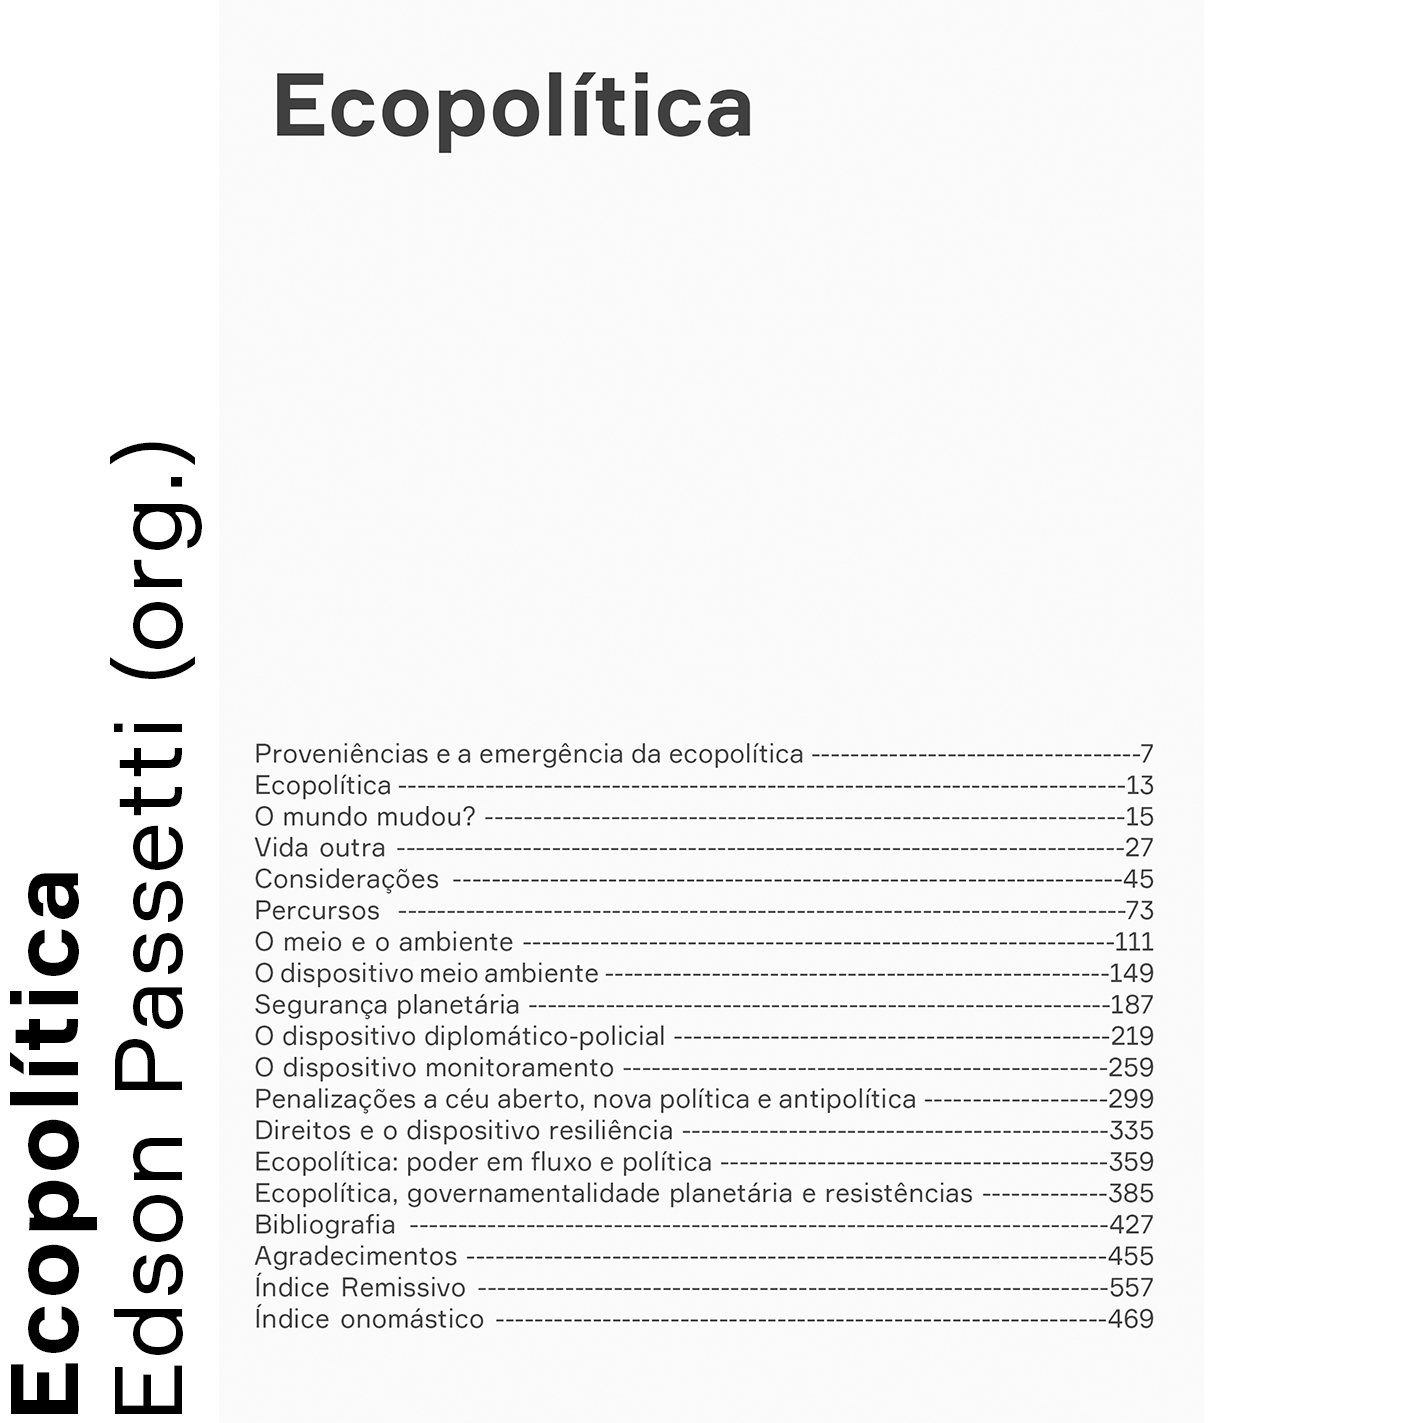
\includegraphics[width=40mm]{./grid2/passetti.jpg}}
\subfloat{
\includegraphics[width=40mm]{./grid2/freud.jpg}}
\subfloat{
\includegraphics[width=40mm]{./grid2/brown.jpg}}\\\hspace*{-.5cm}
\vspace{.5cm}
\subfloat{
\includegraphics[width=40mm]{./grid2/jacobs.jpg}}
\subfloat{
\includegraphics[width=40mm]{./grid2/wpa.jpg}}
\subfloat{
\includegraphics[width=40mm]{./grid2/jazz.jpg}}\\\hspace*{-.5cm}
\vspace{.5cm}
\subfloat{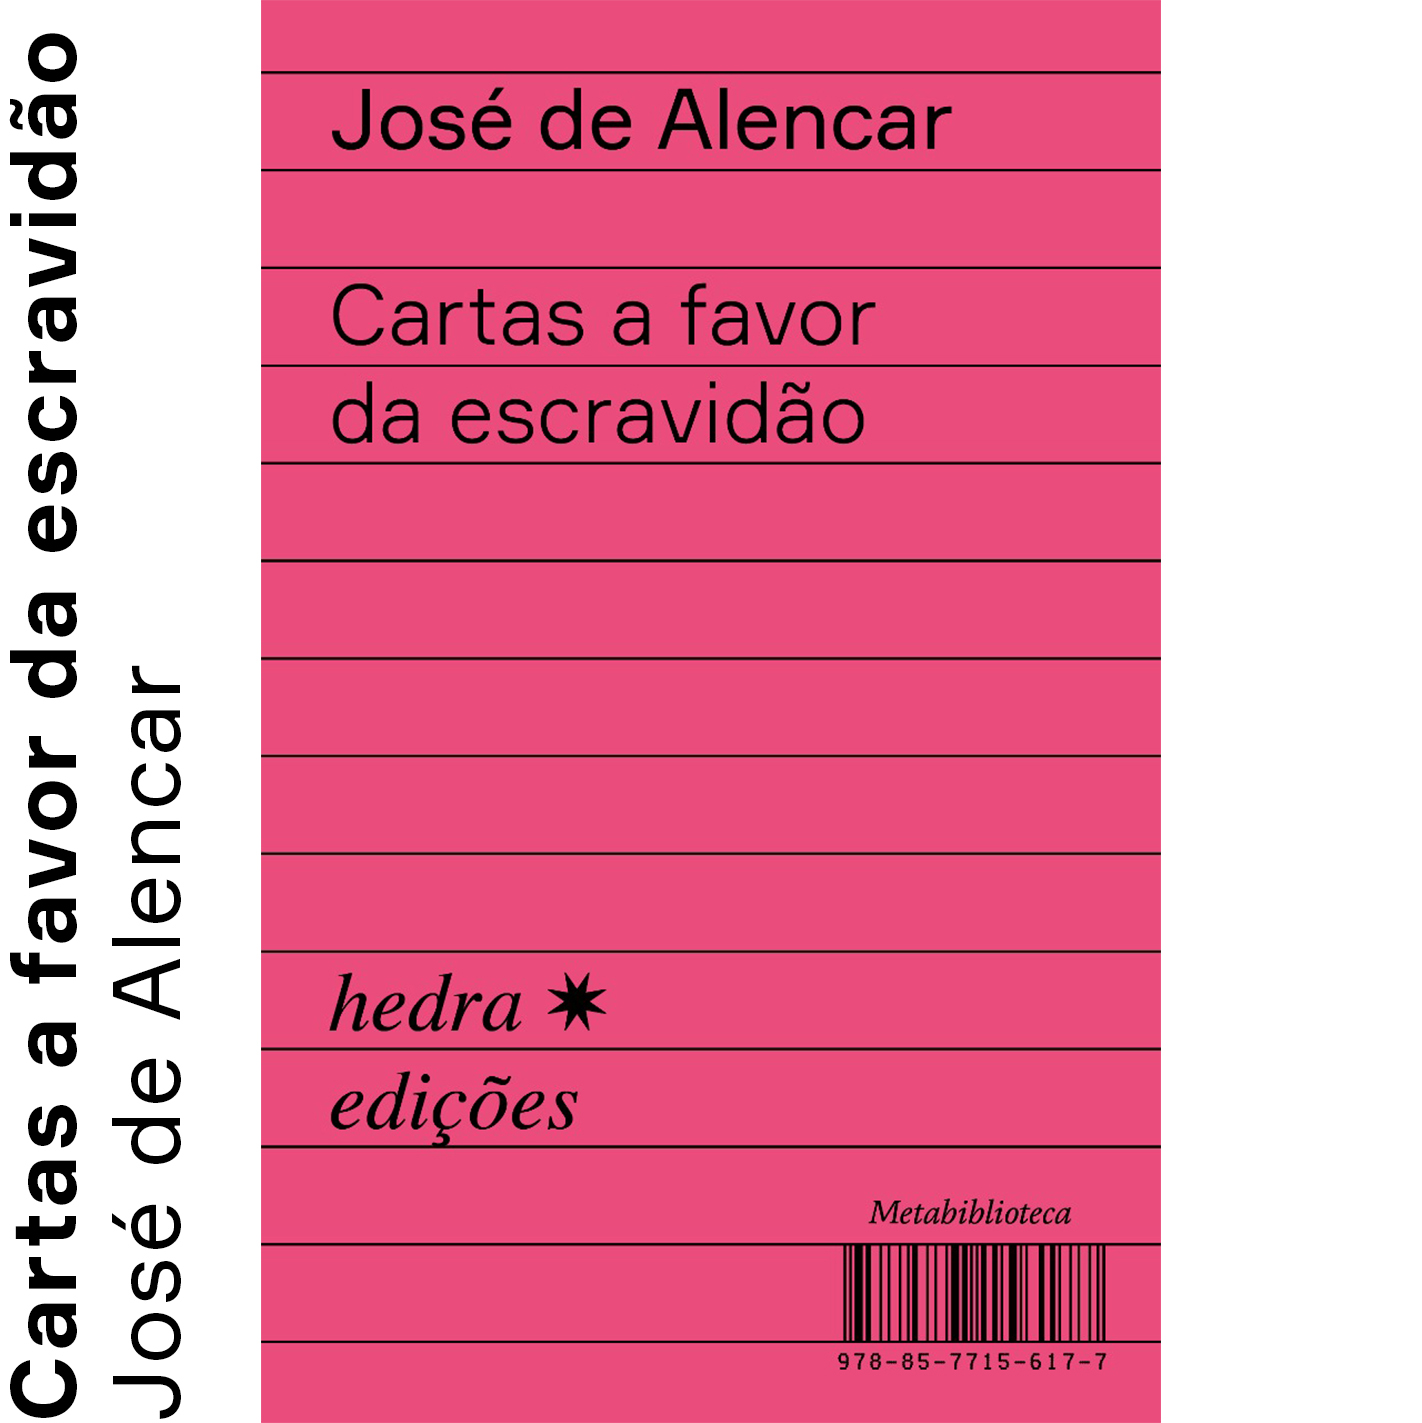
\includegraphics[width=40mm]{./grid2/alencar.jpg}}
\subfloat{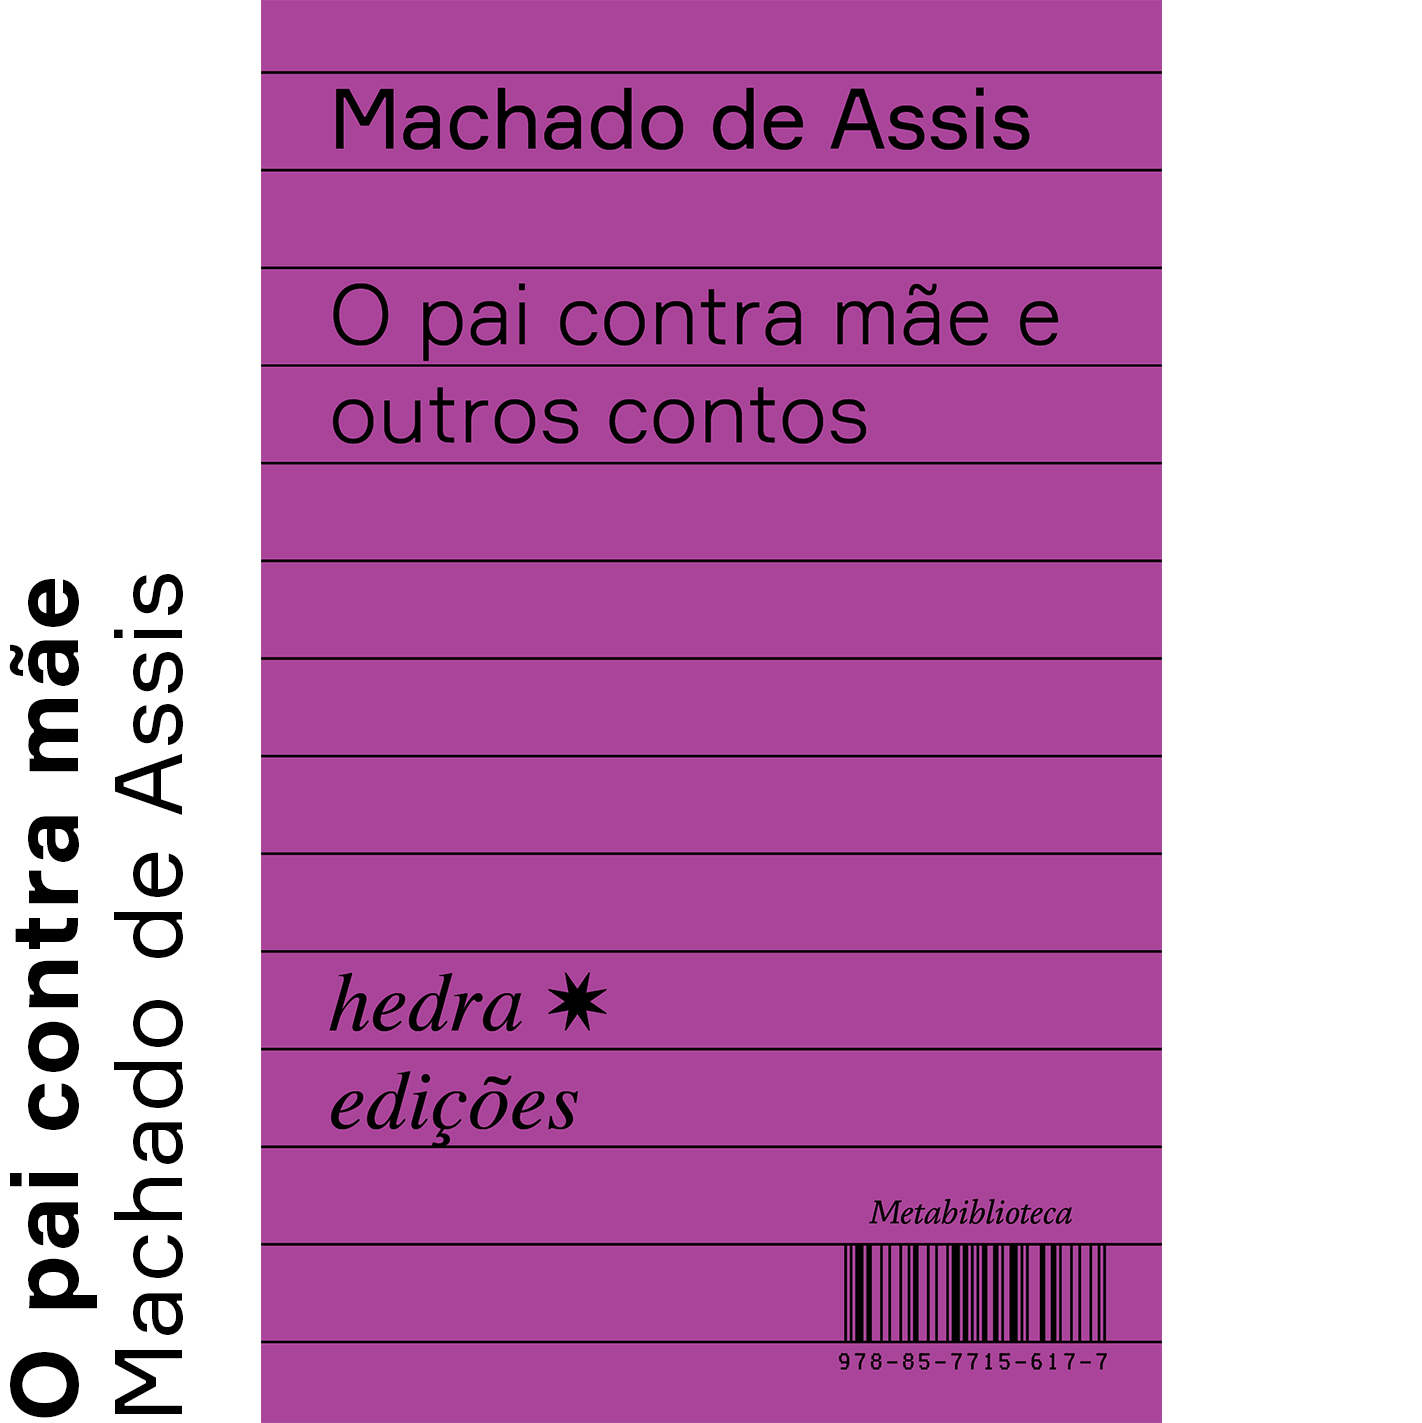
\includegraphics[width=40mm]{./grid2/machado.jpg}}
\subfloat{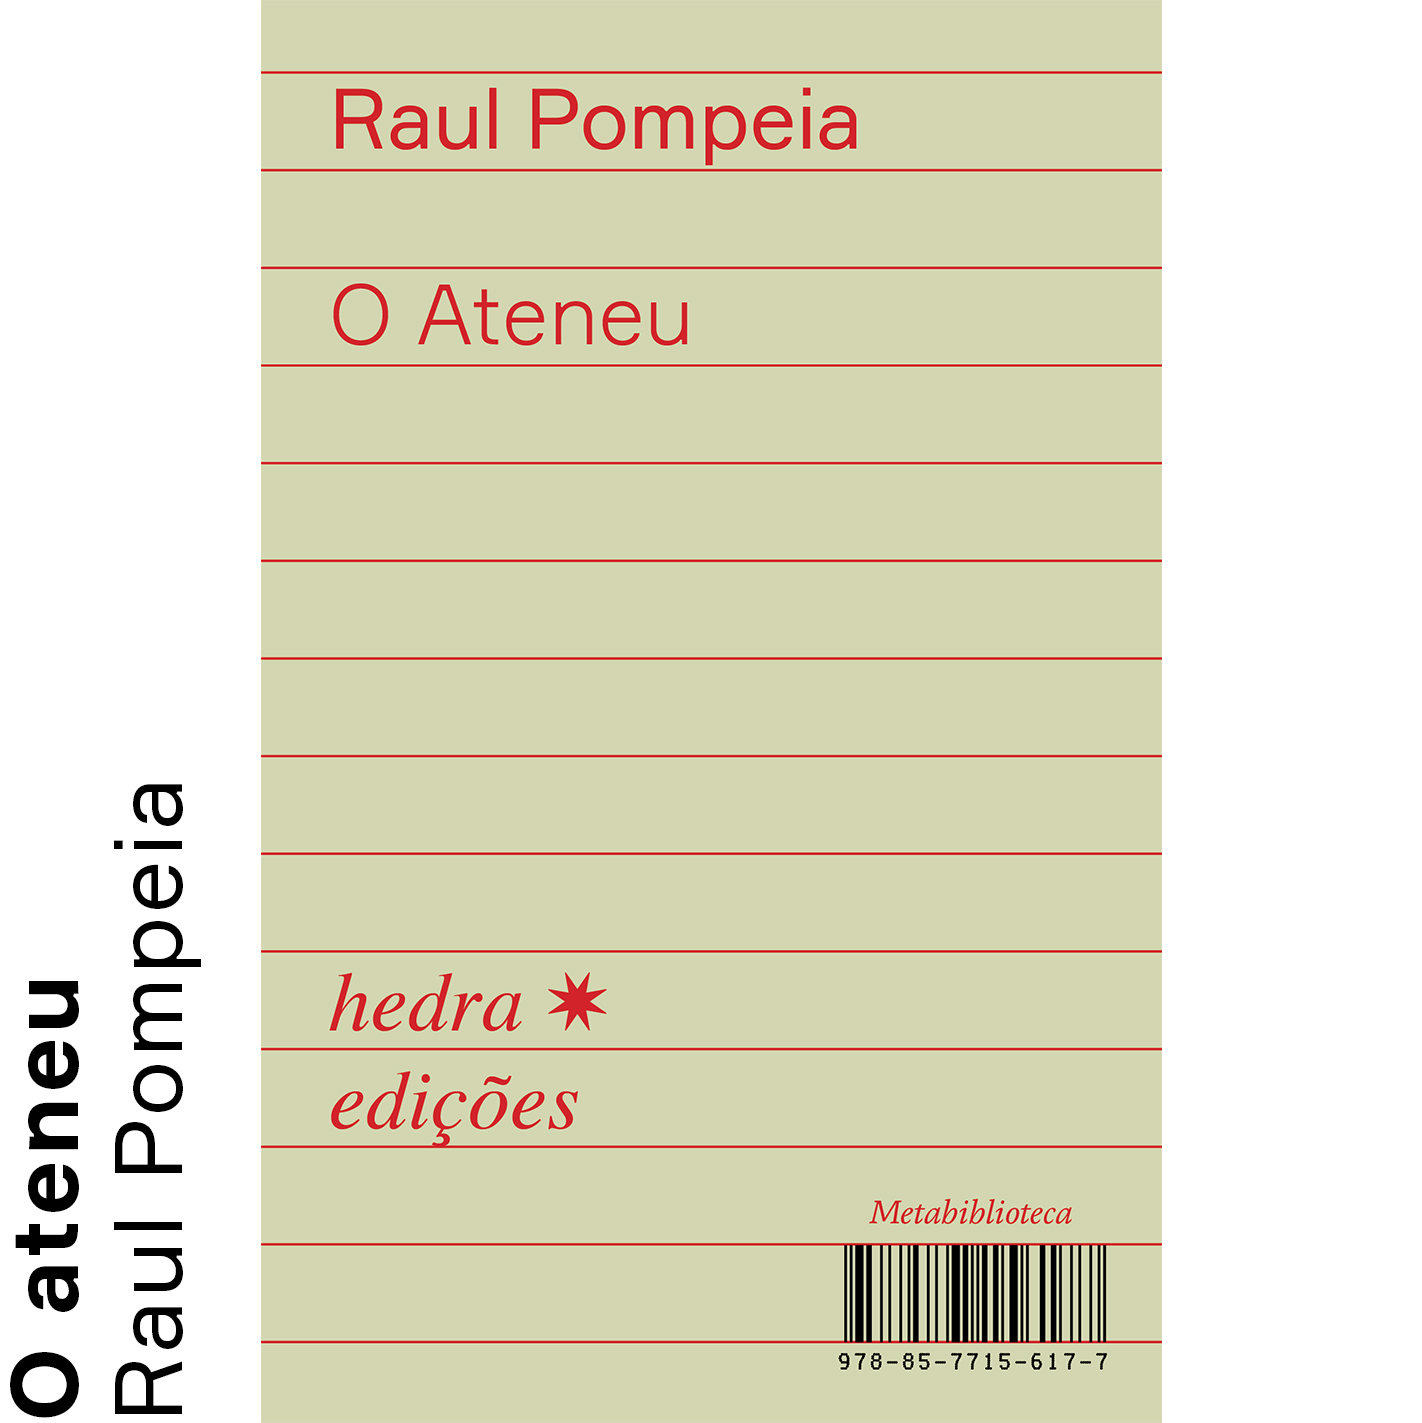
\includegraphics[width=40mm]{./grid2/ateneu.jpg}}\\\hspace*{-.5cm}
\vspace{.5cm}
\subfloat{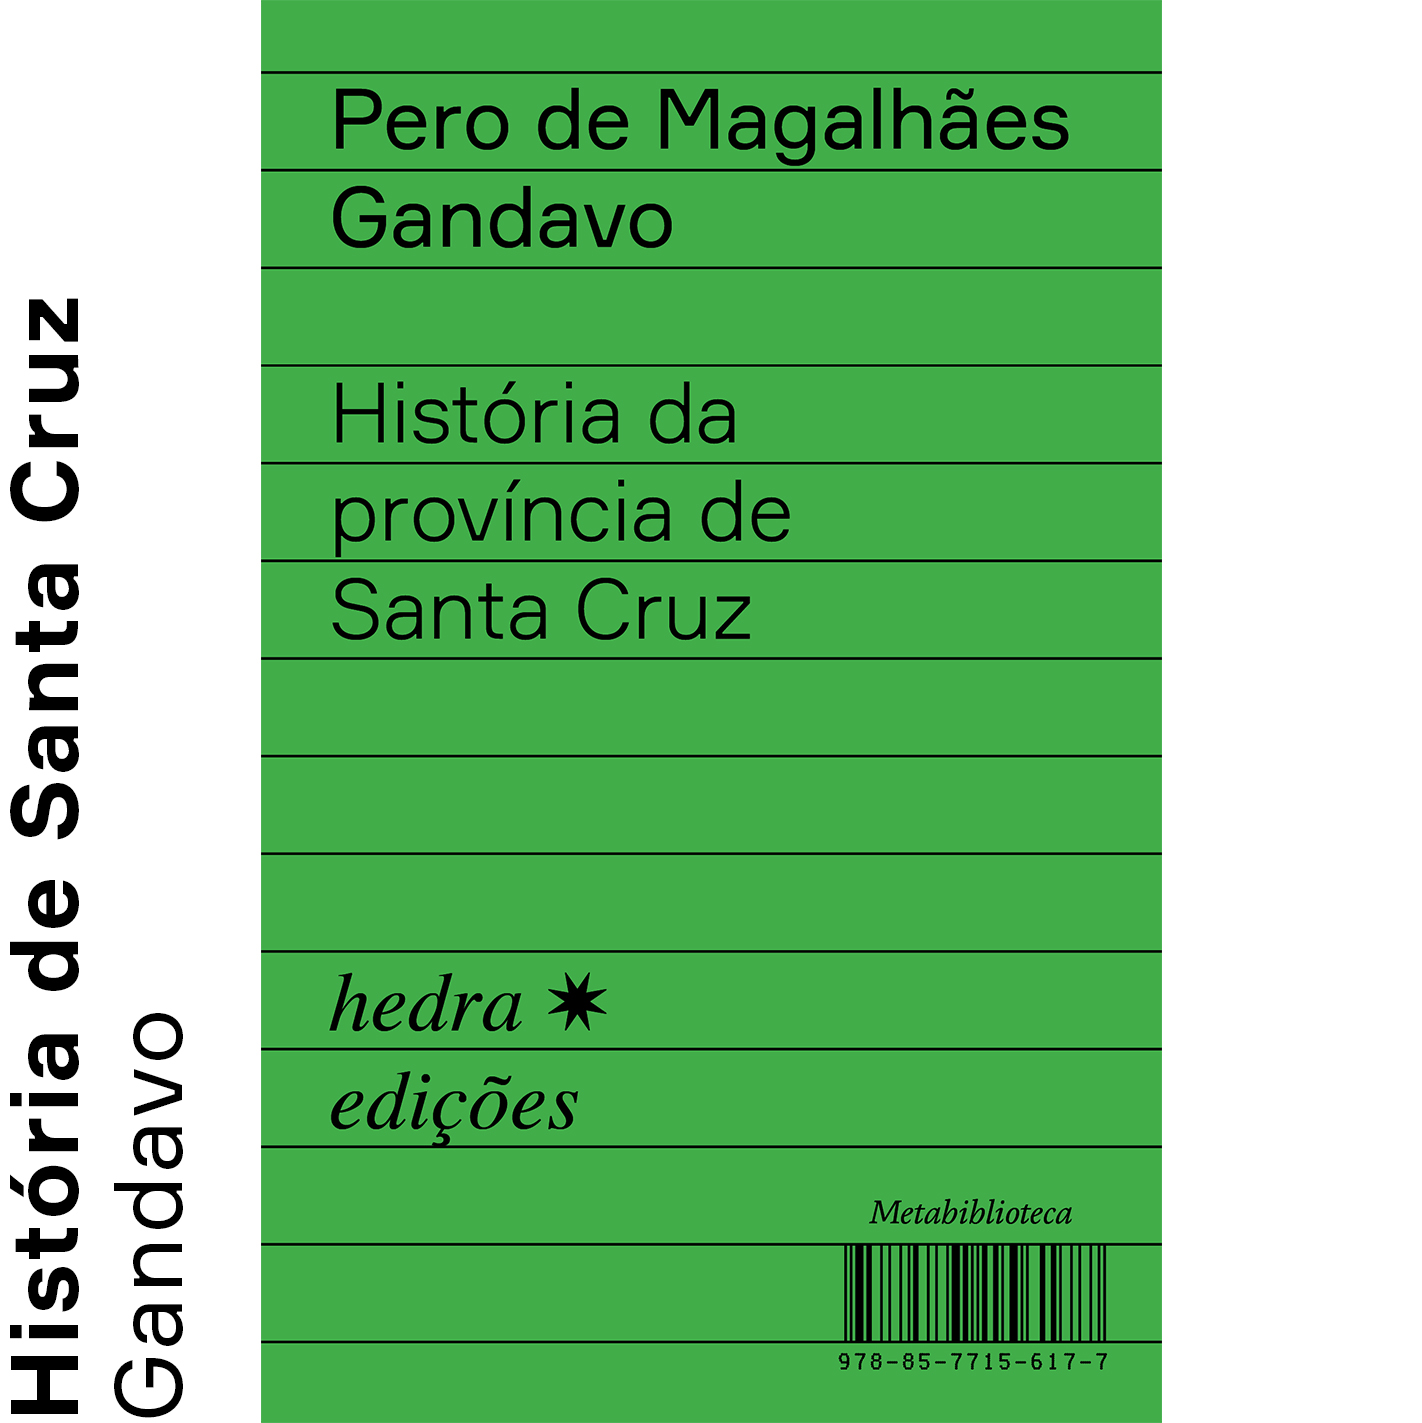
\includegraphics[width=40mm]{./grid2/gandavo.jpg}}
\subfloat{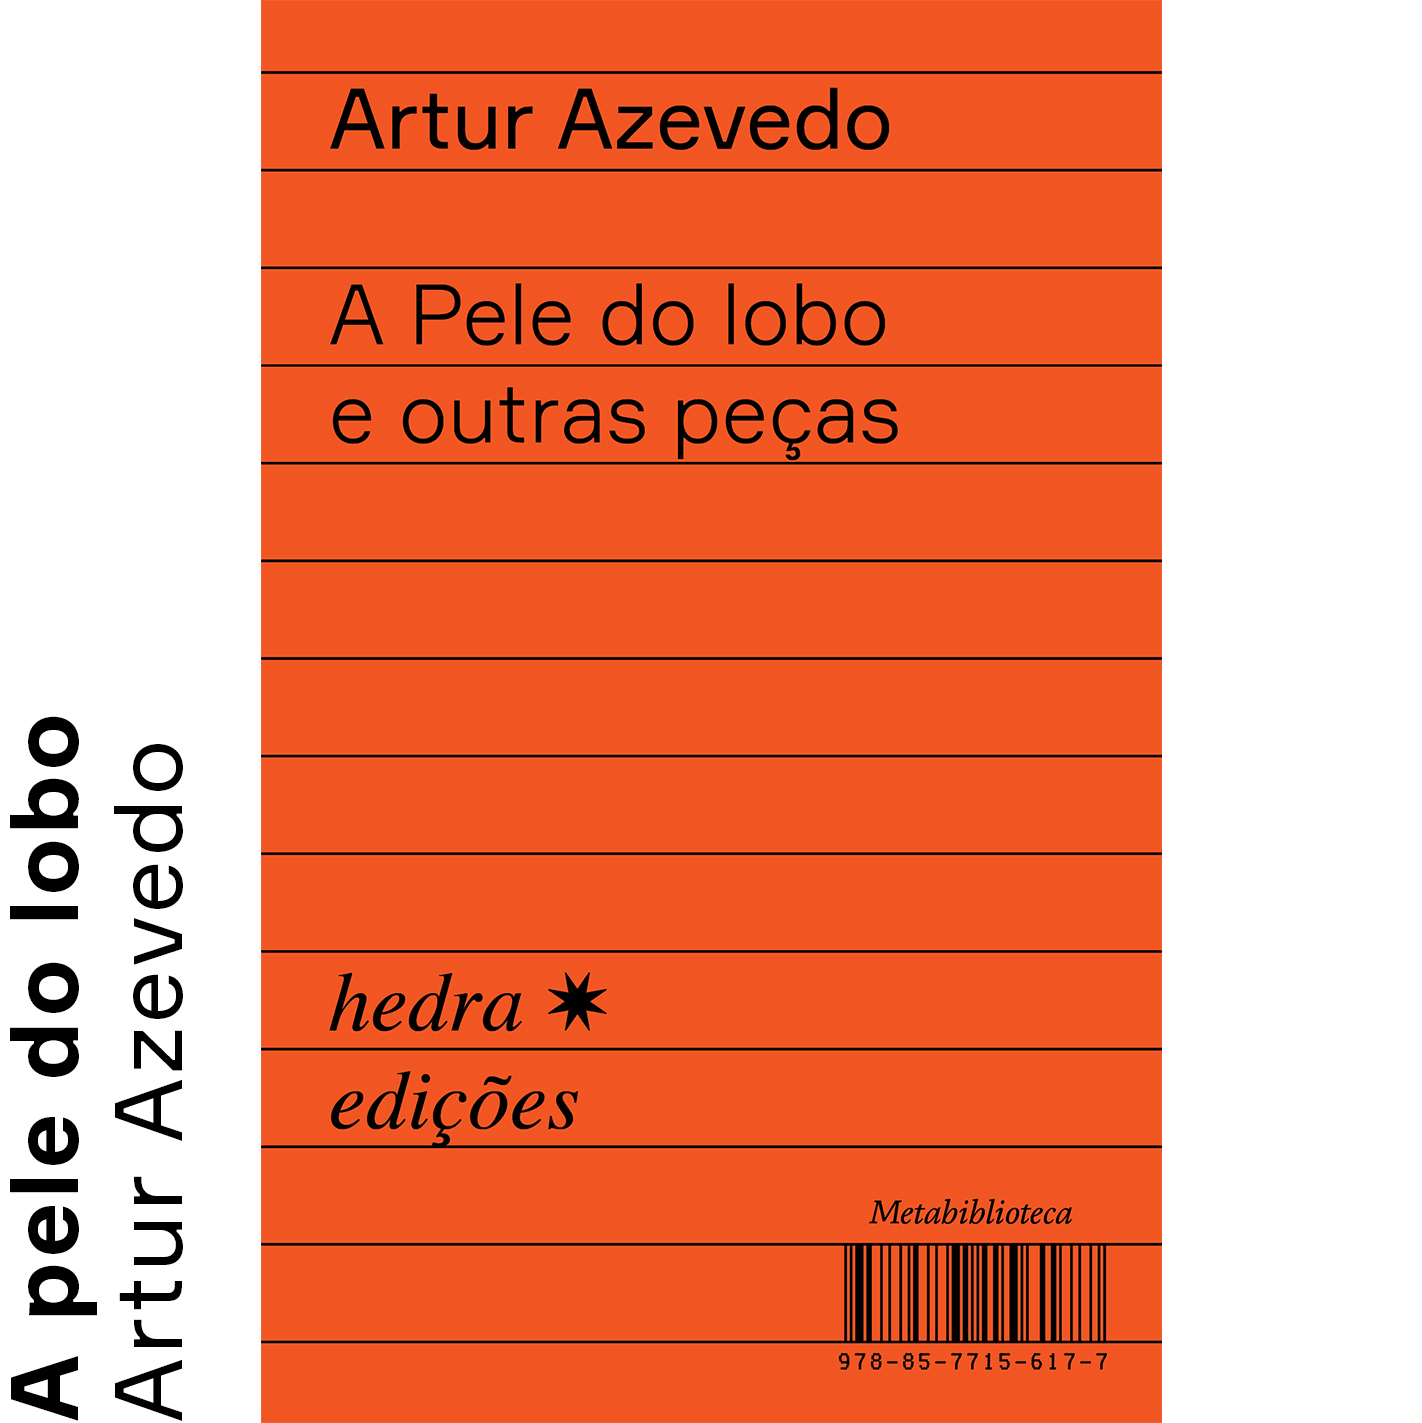
\includegraphics[width=40mm]{./grid2/azevedo.jpg}}
\subfloat{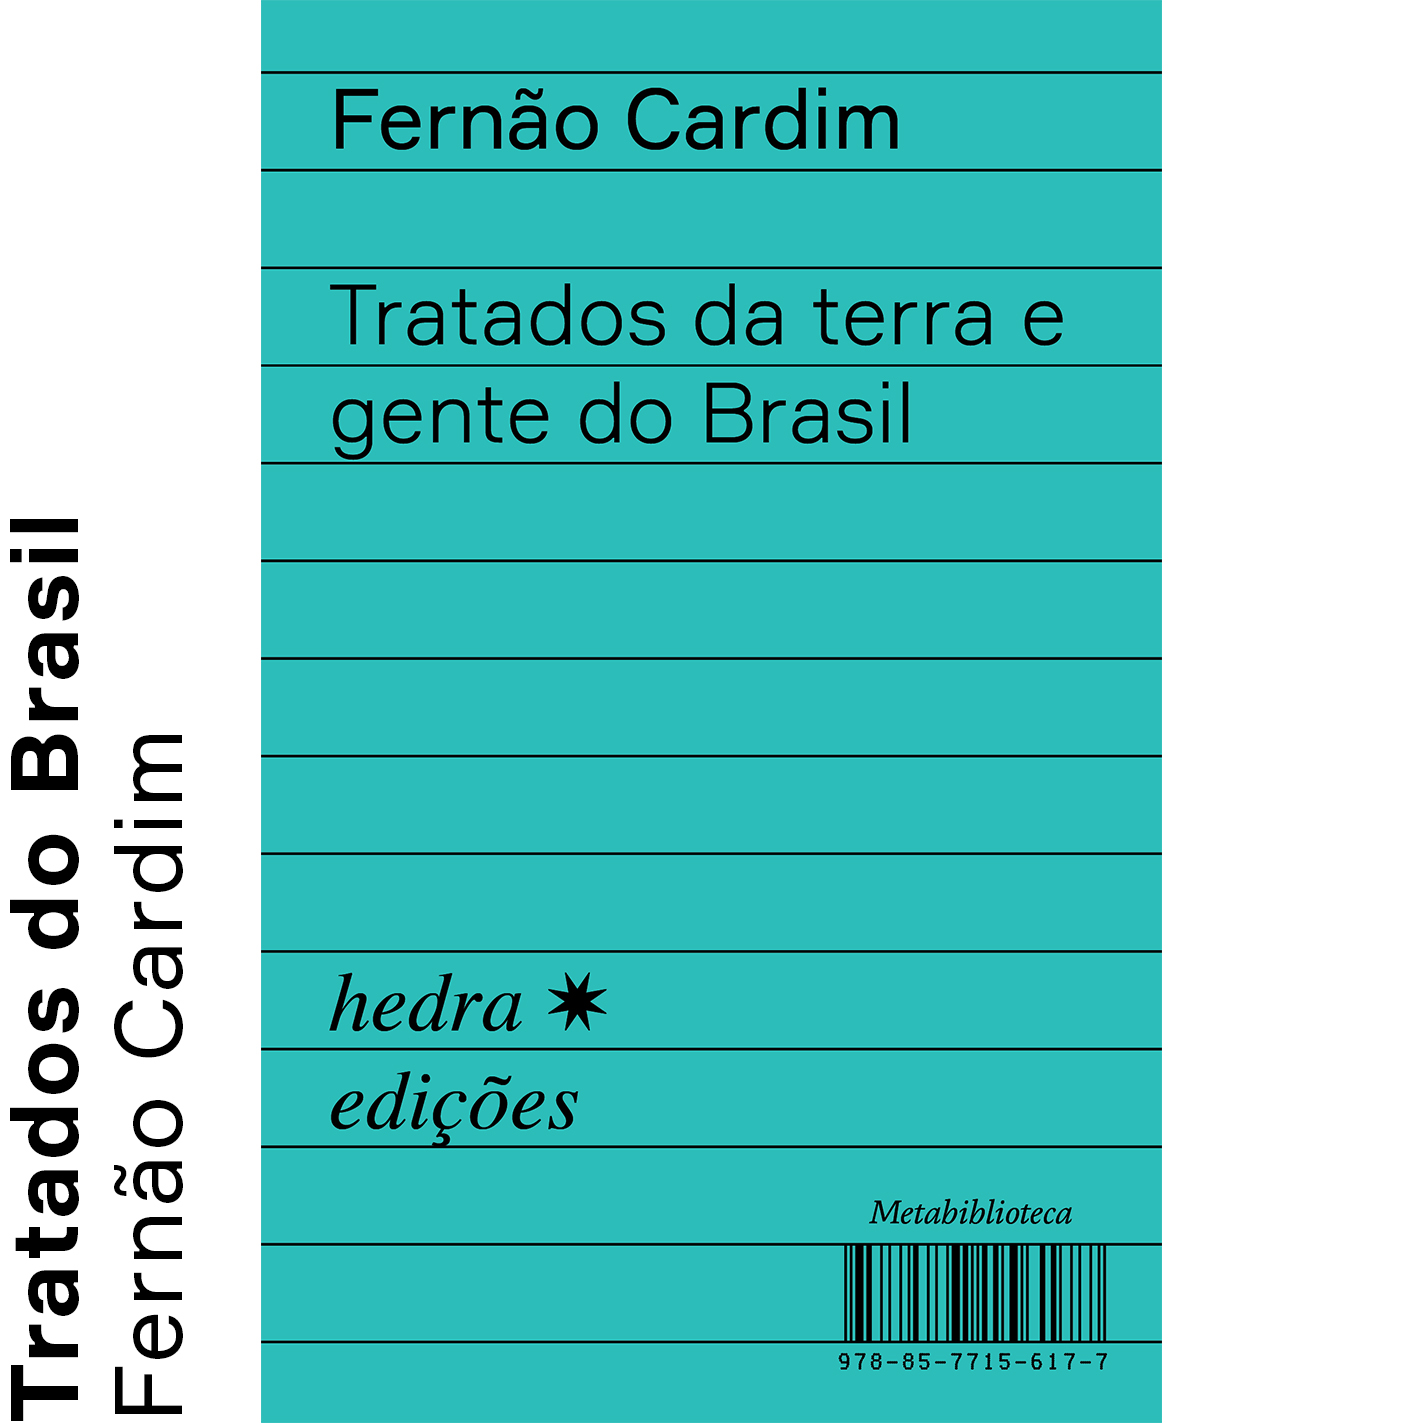
\includegraphics[width=40mm]{./grid2/cardim.jpg}}\\
\end{tabular}
\end{figure}

\pagebreak

\begin{figure}[!htbp]
\begin{tabular}{cccc}

\vspace{.5cm}
\hspace*{-.5cm}
\subfloat{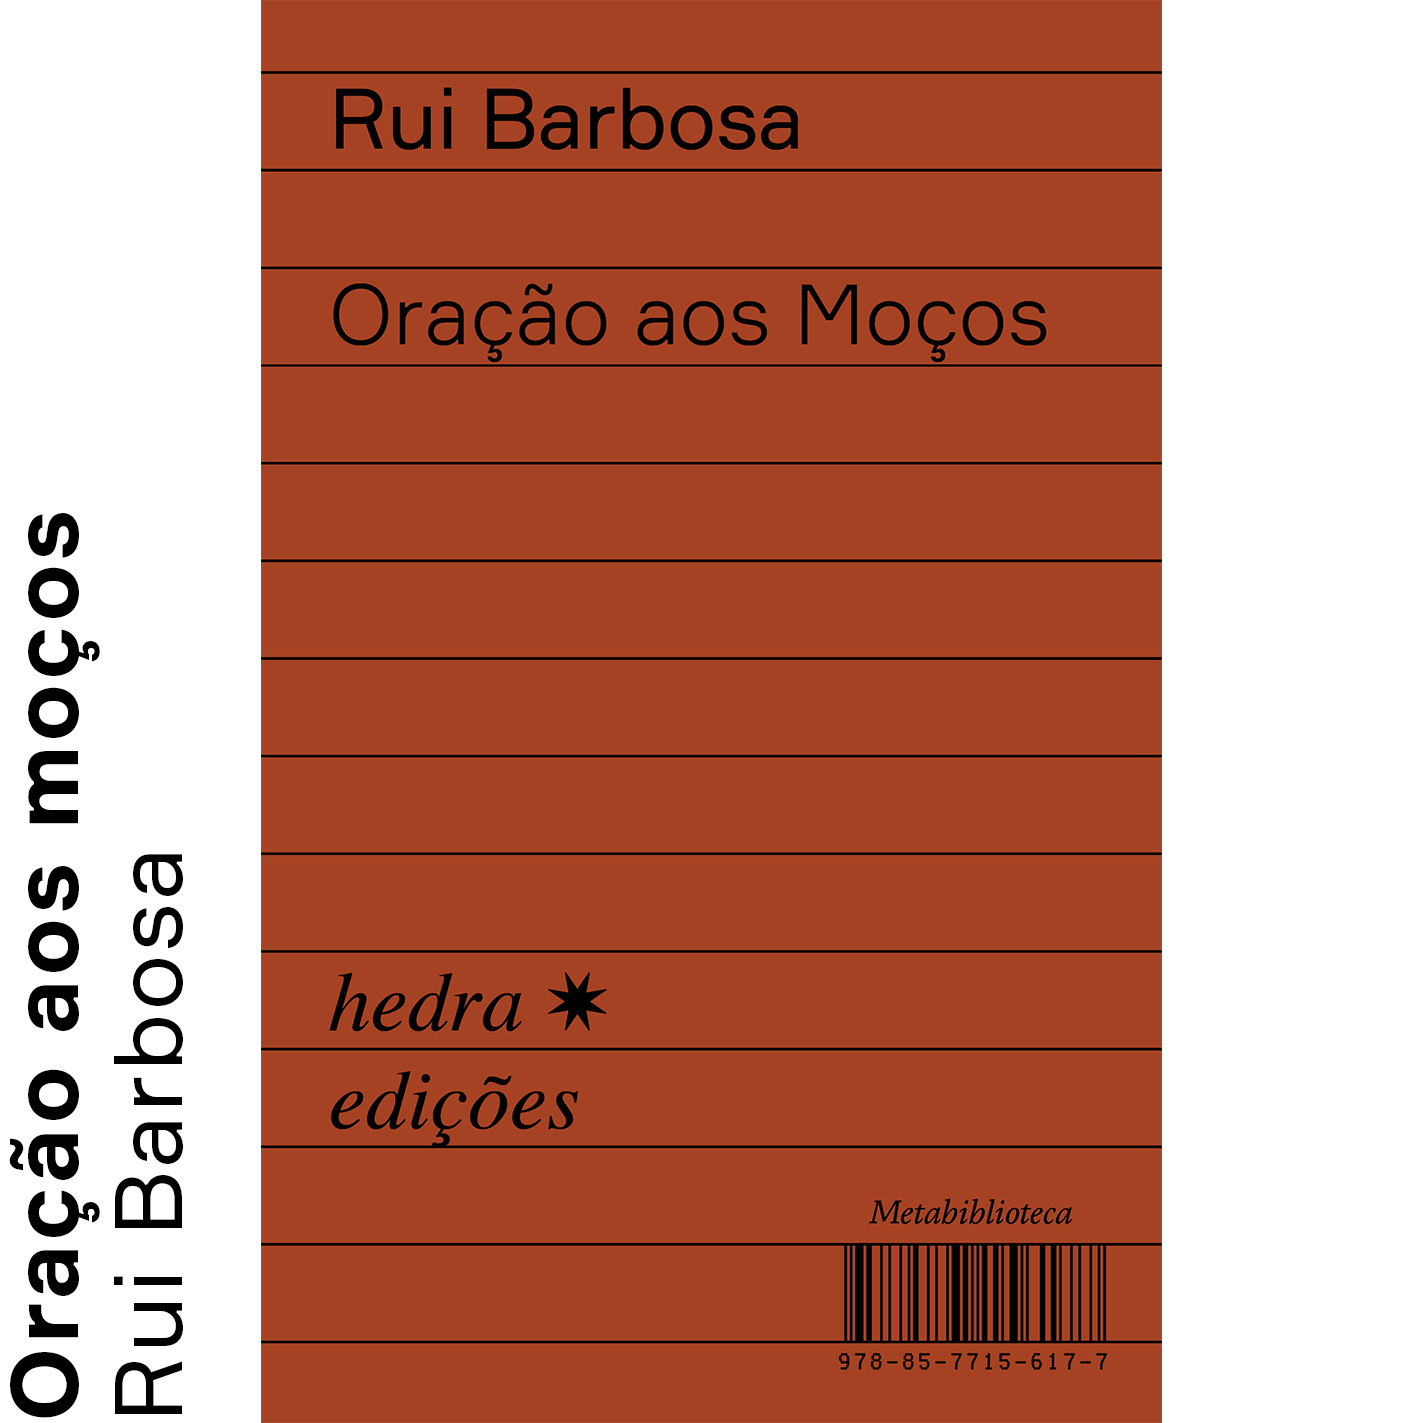
\includegraphics[width=40mm]{./grid2/barbosa.jpg}}
\subfloat{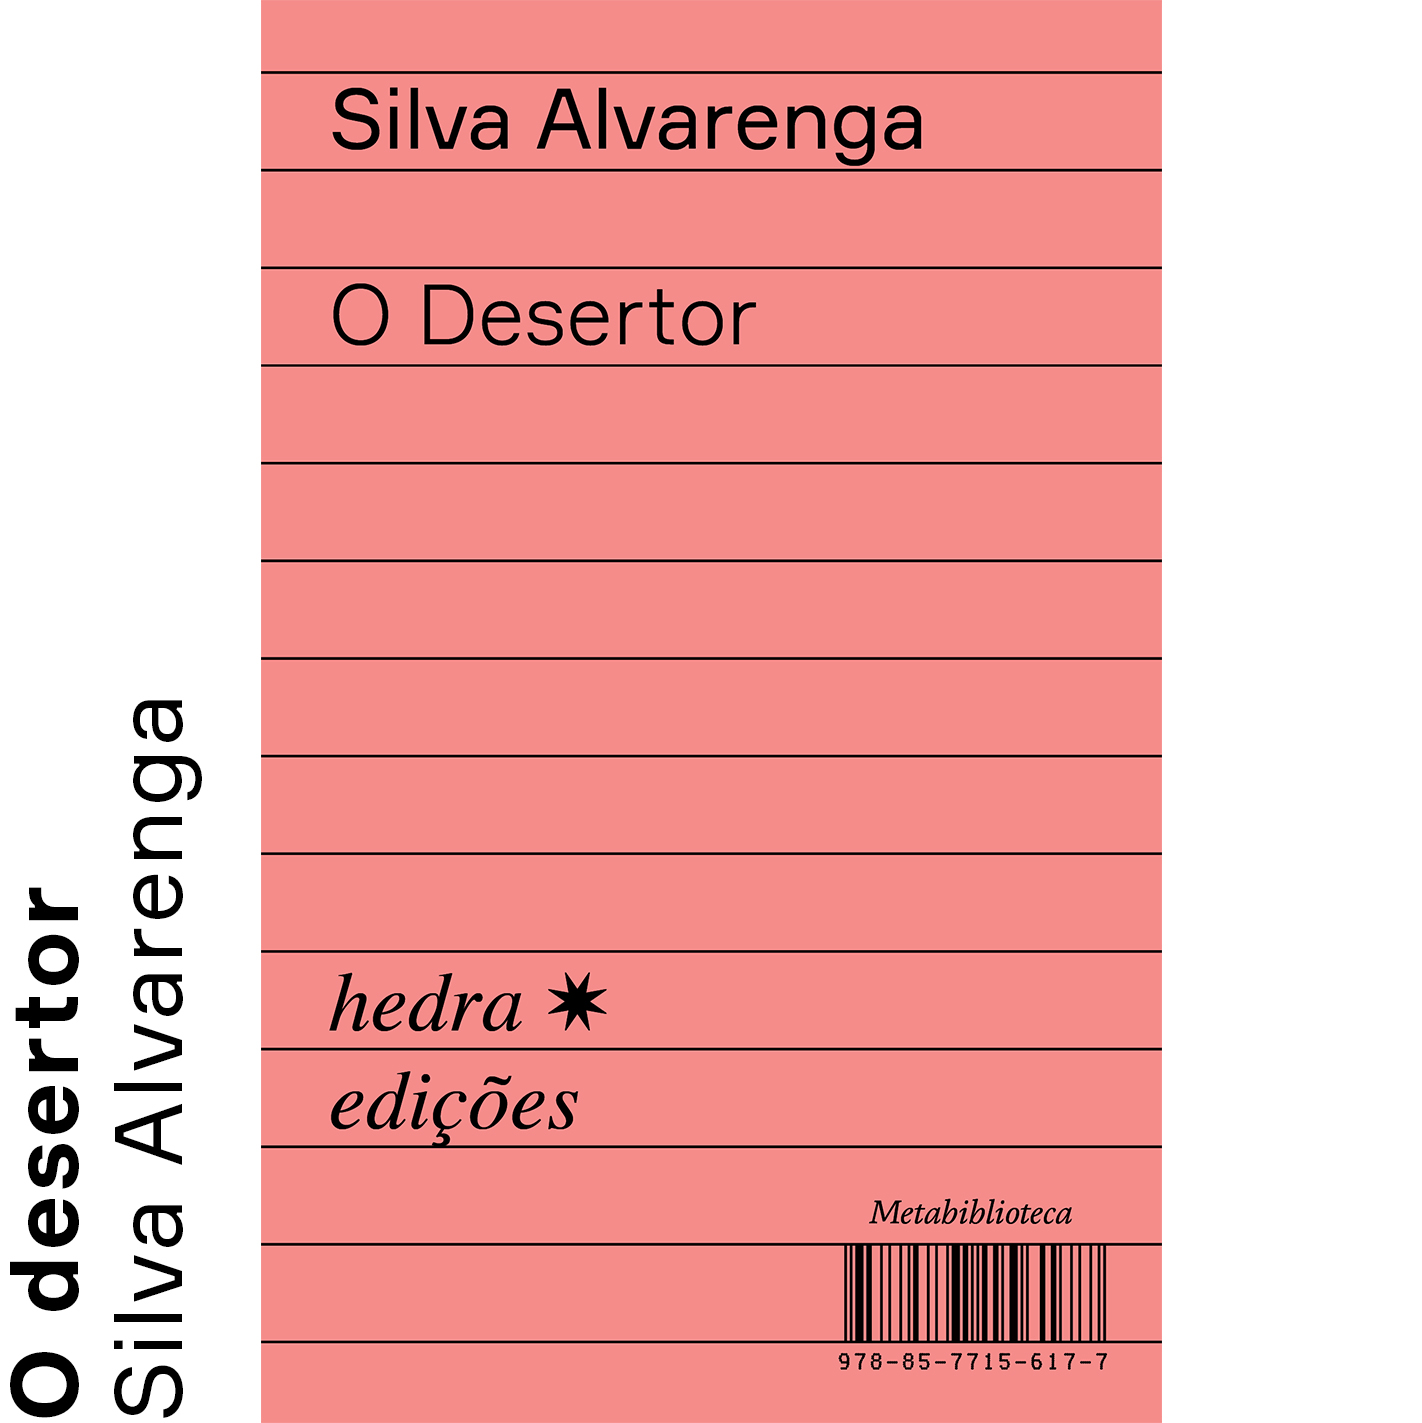
\includegraphics[width=40mm]{./grid2/desertor.jpg}}
\subfloat{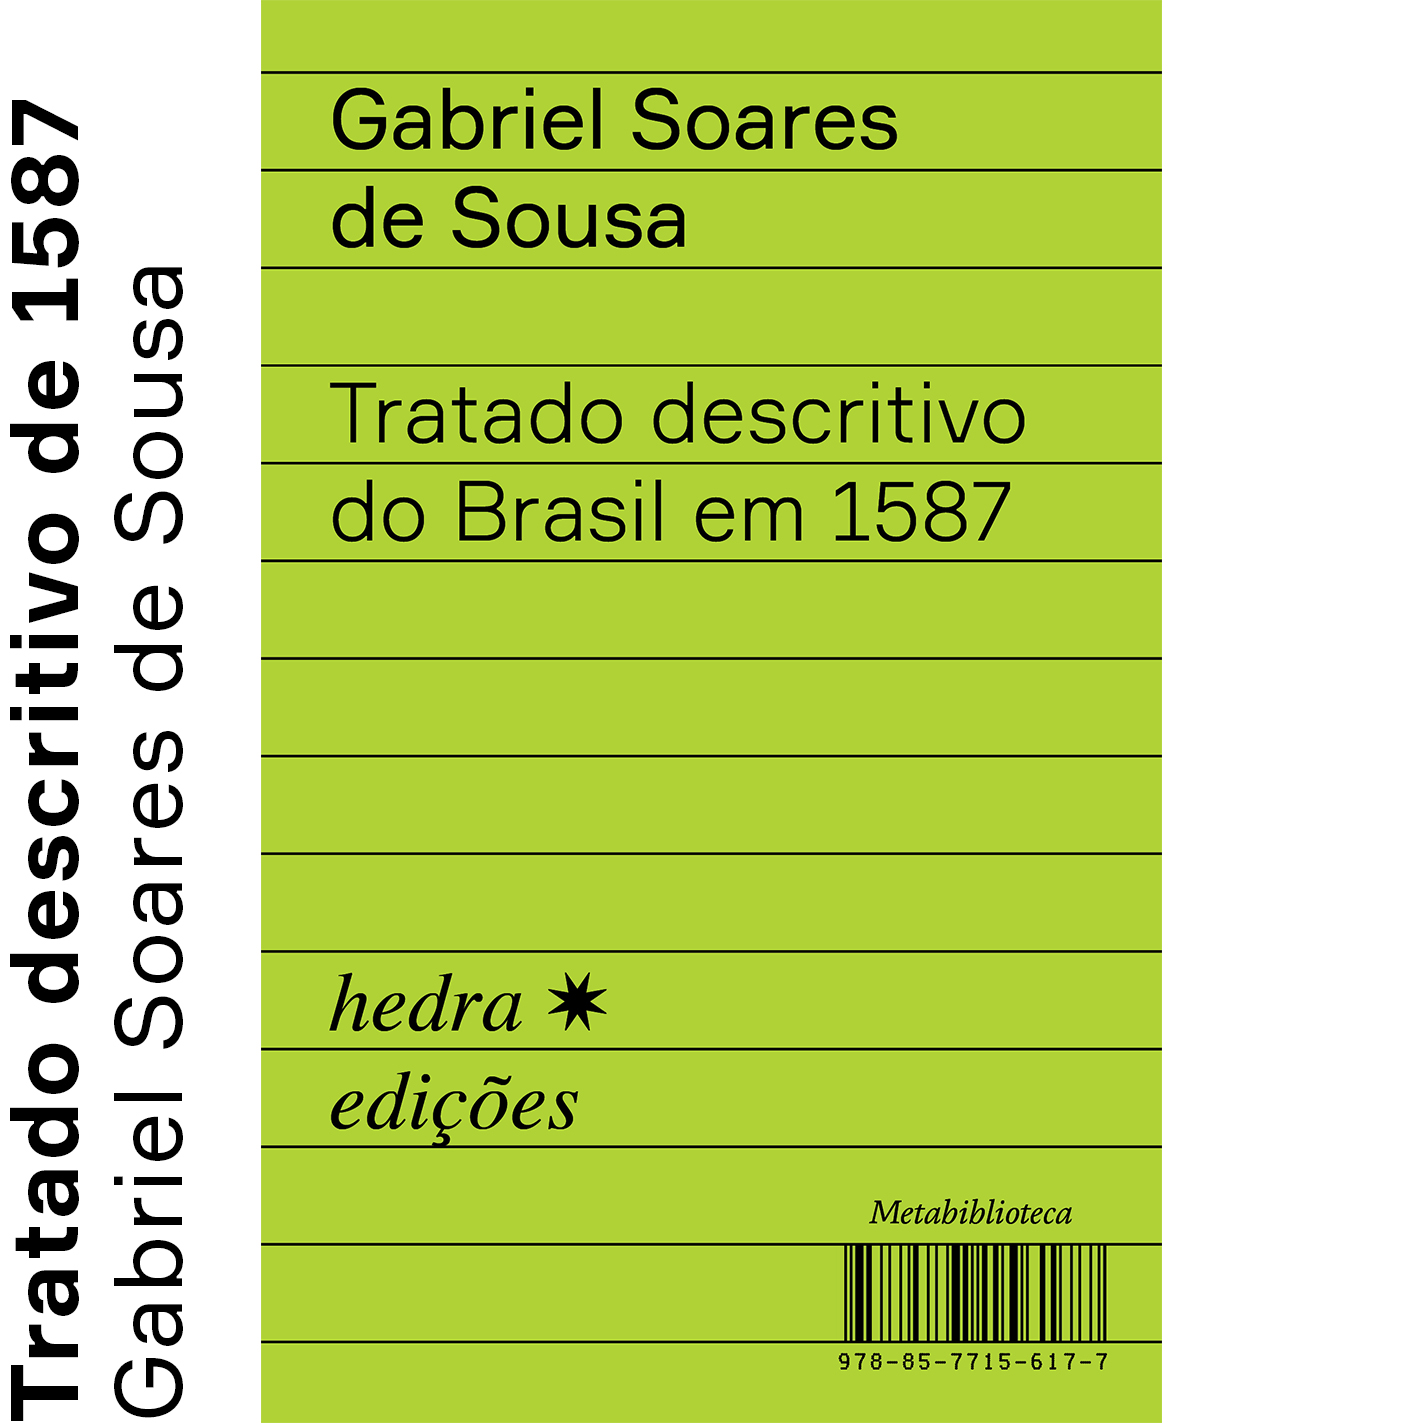
\includegraphics[width=40mm]{./grid2/tratado.jpg}}\\\hspace*{-.5cm}
\vspace{.5cm}
\subfloat{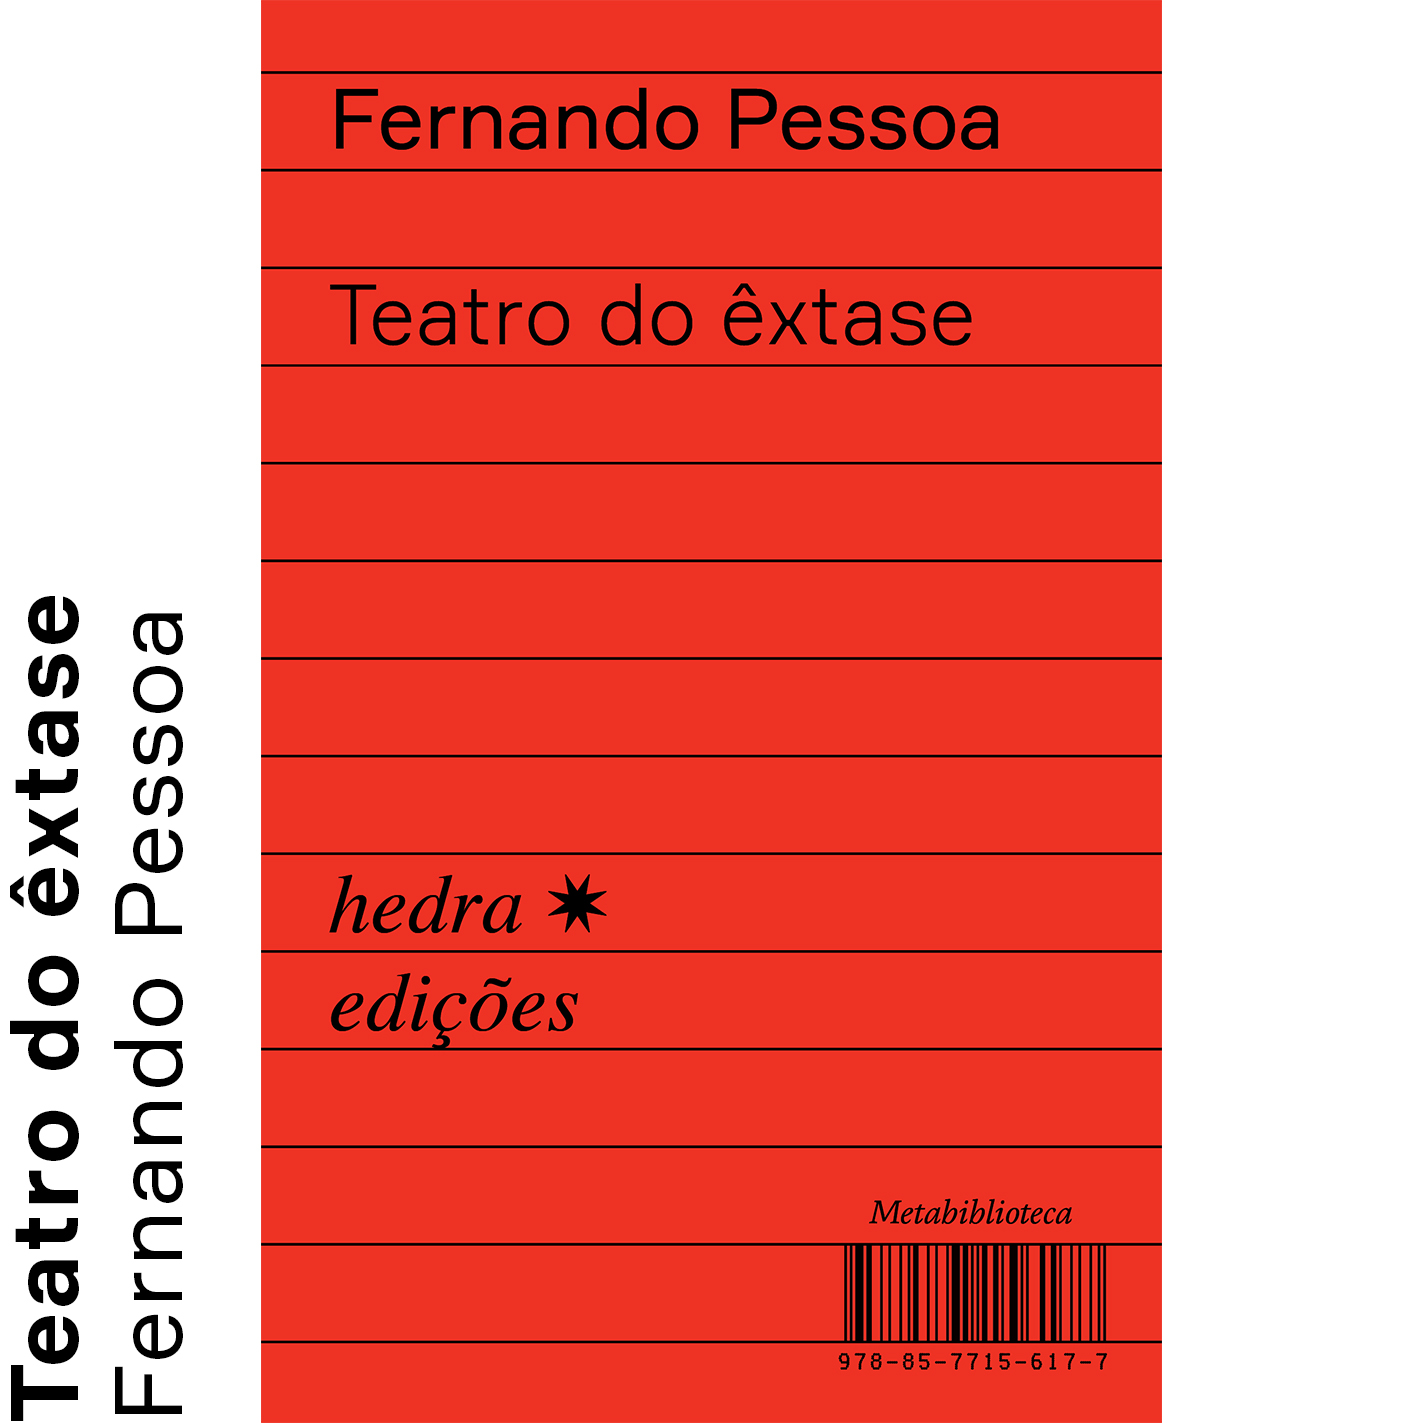
\includegraphics[width=40mm]{./grid2/pessoa.jpg}}
\subfloat{
\includegraphics[width=40mm]{./grid2/lovecraft.jpg}}
\subfloat{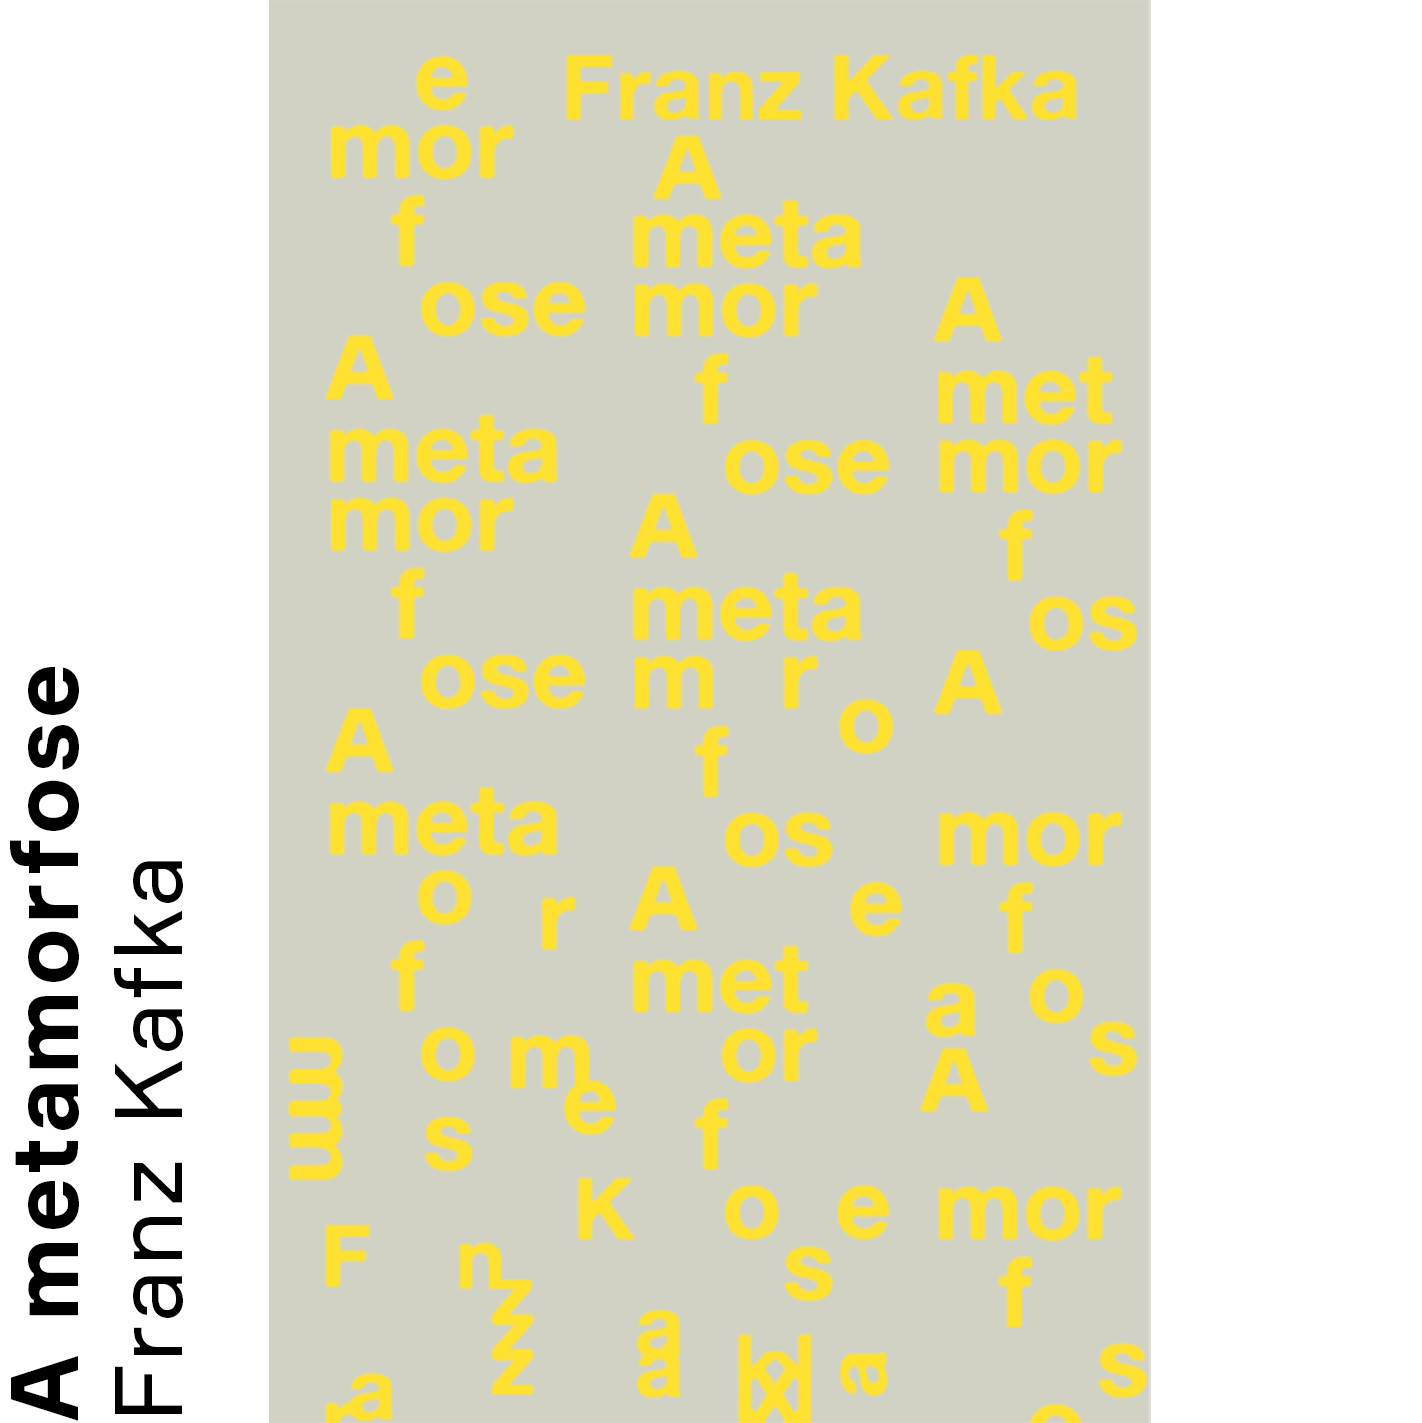
\includegraphics[width=40mm]{./grid2/kafka.jpg}}\\\hspace*{-.5cm}
\vspace{.5cm}
\subfloat{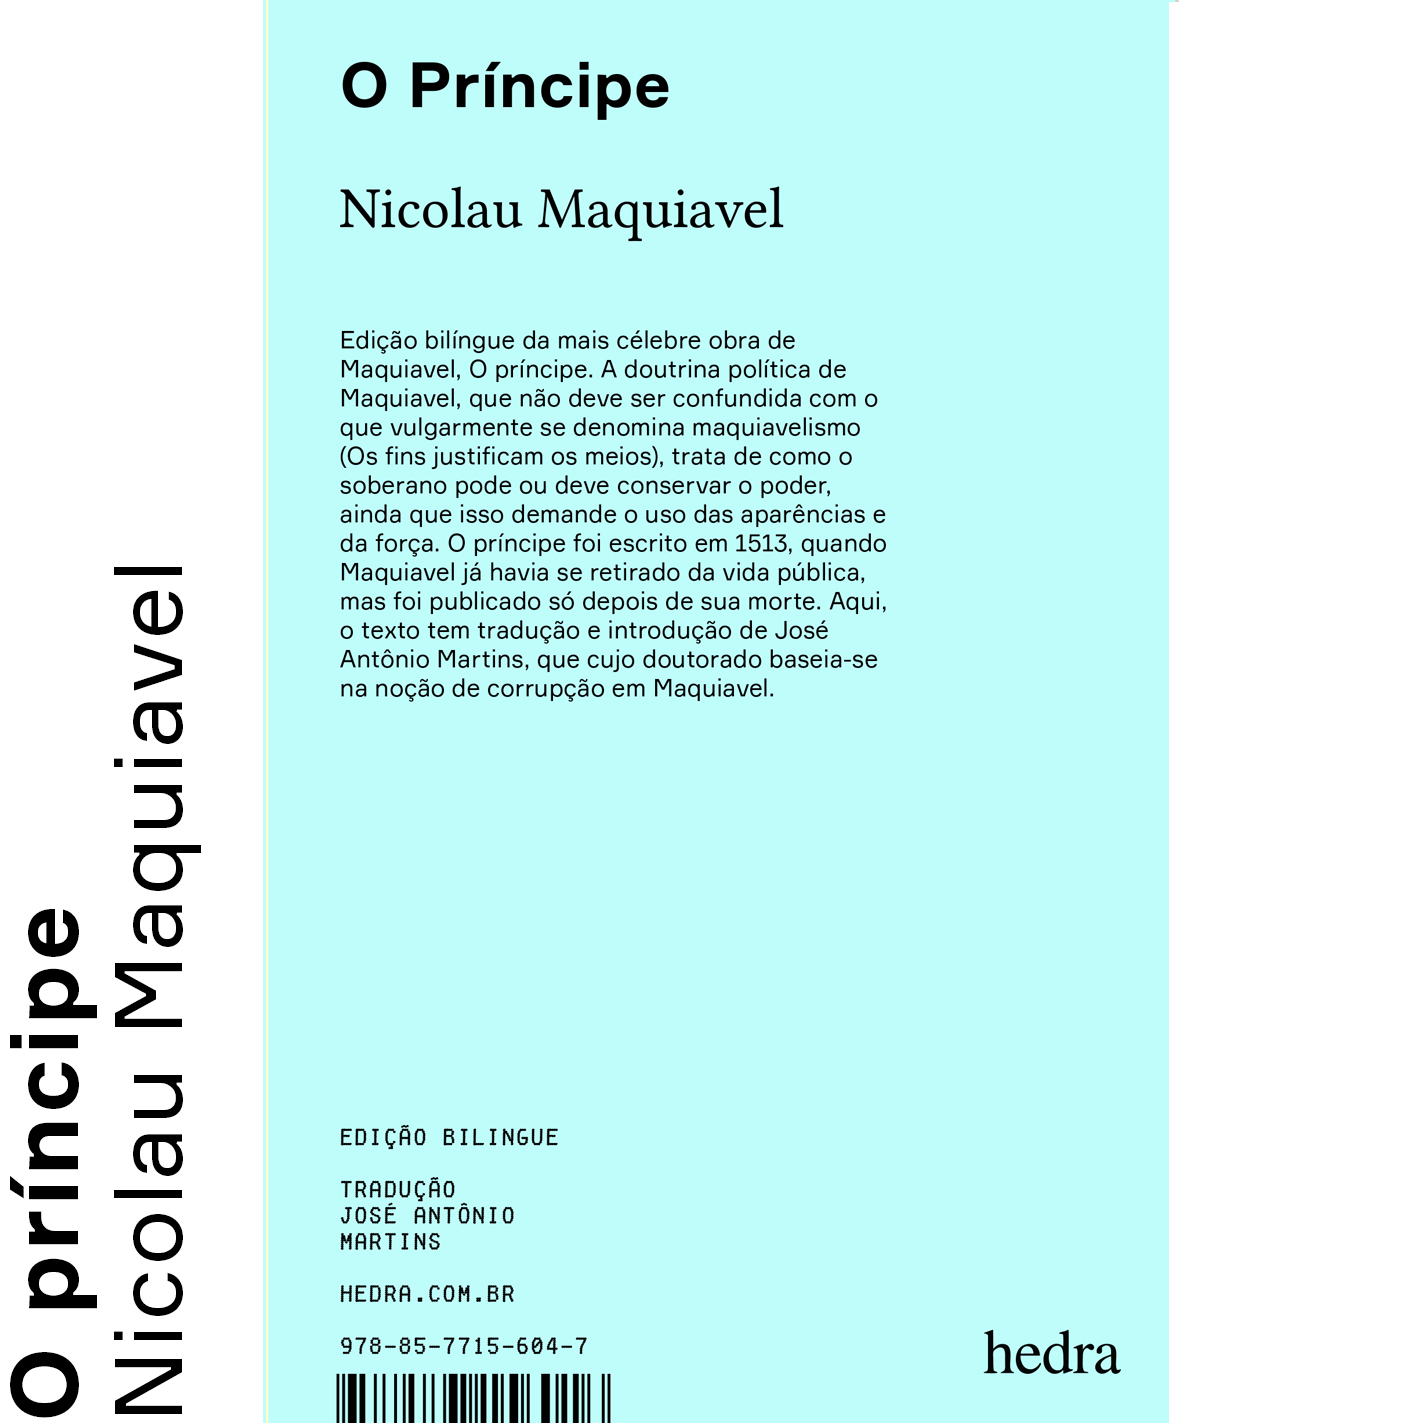
\includegraphics[width=40mm]{./grid2/maquiavel.jpg}}
\subfloat{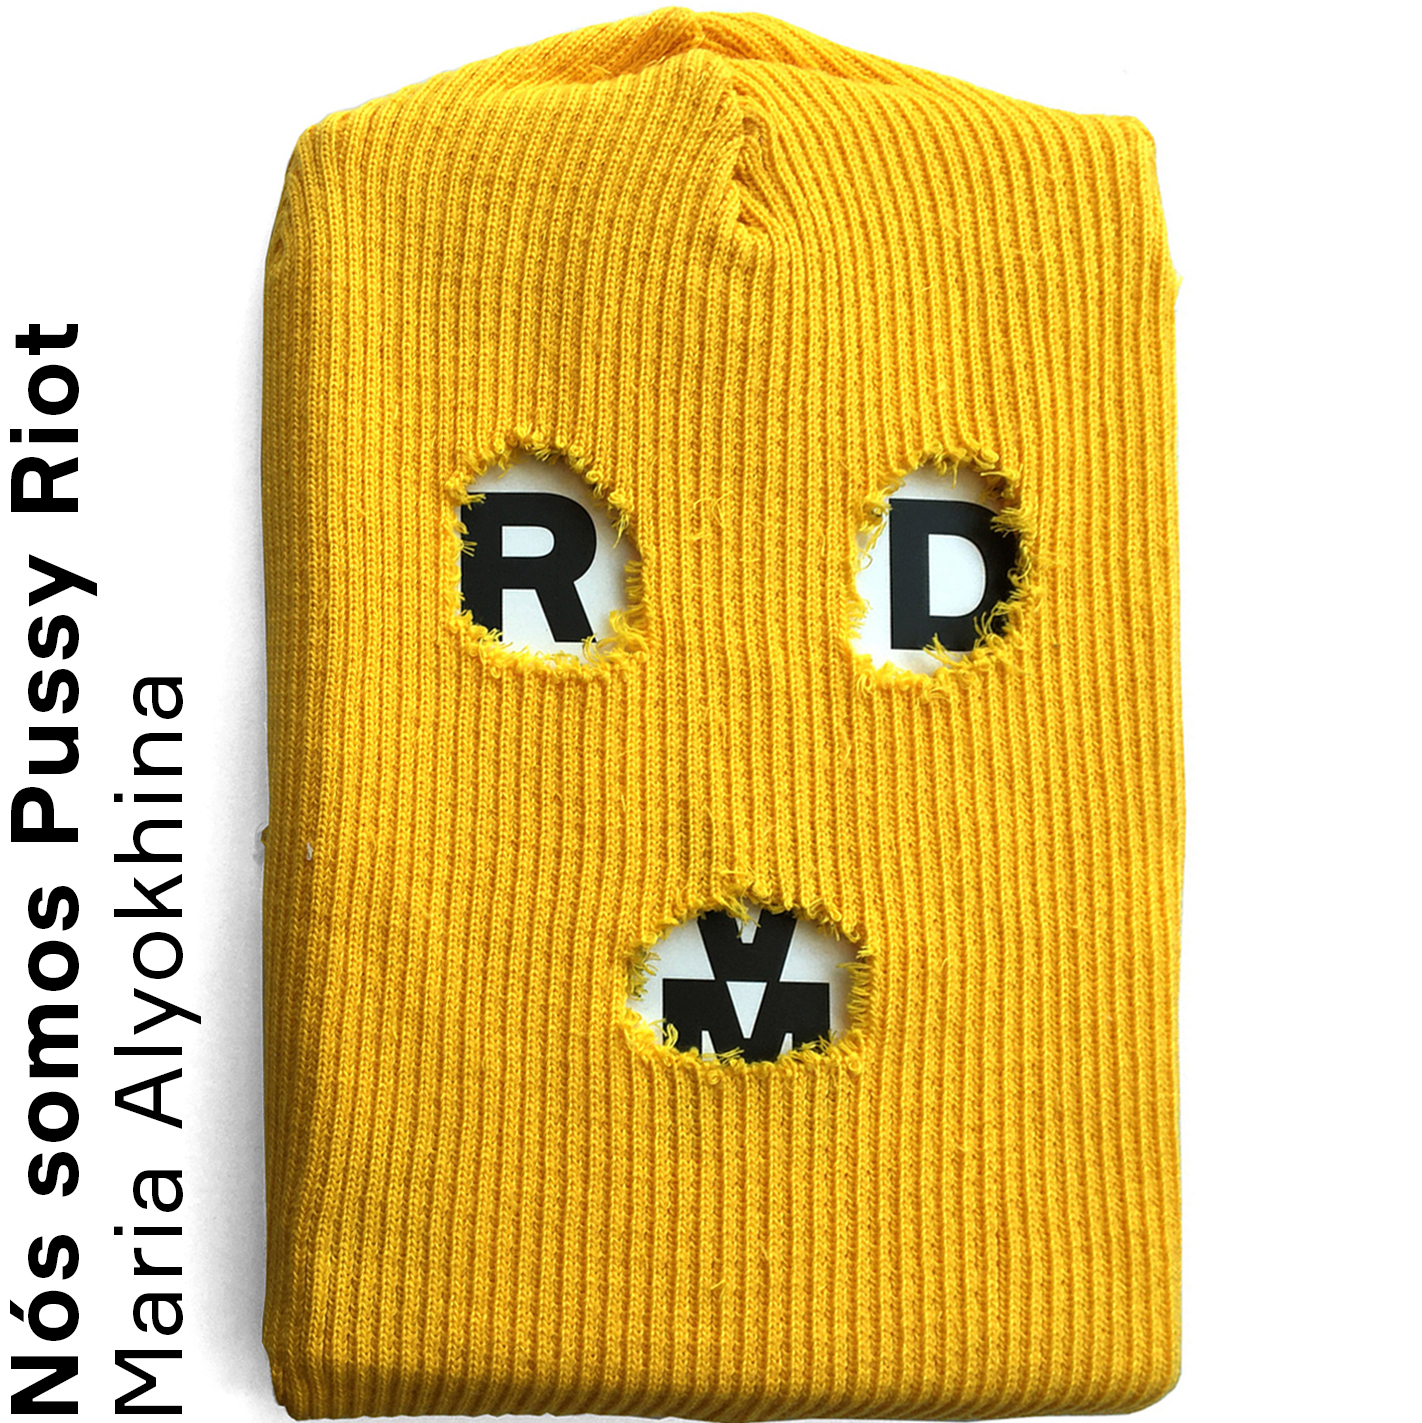
\includegraphics[width=40mm]{./grid2/riot.jpg}}
\subfloat{
\includegraphics[width=40mm]{./grid2/butler.jpg}}\\\hspace*{-.5cm}
\vspace{.5cm}
\subfloat{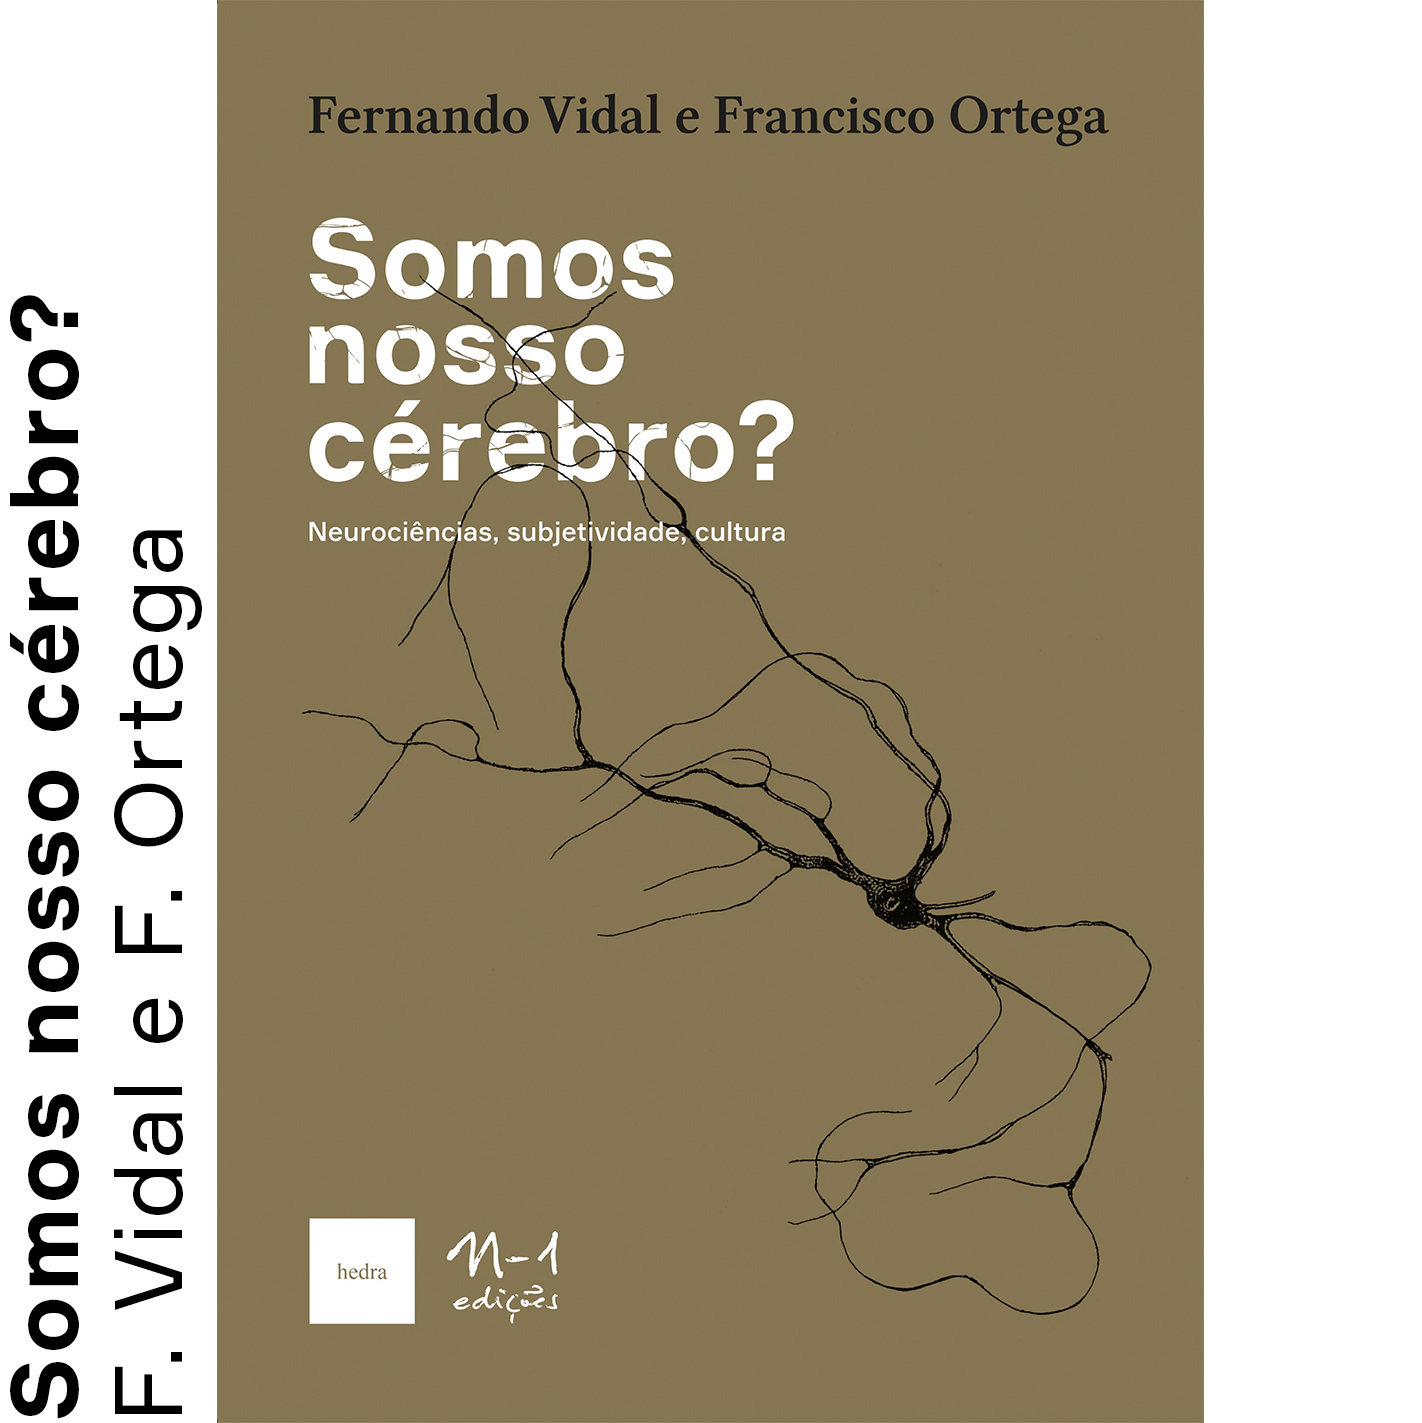
\includegraphics[width=40mm]{./grid2/cerebro.jpg}}
\subfloat{
\includegraphics[width=40mm]{./grid2/gozo.jpg}}
\subfloat{
\includegraphics[width=40mm]{./grid2/lazzarato.jpg}}\\
\end{tabular}
\end{figure}

\pagebreak

\begin{figure}[!htbp]
\begin{tabular}{cccc}

\vspace{.5cm}
\hspace*{-.5cm}
\subfloat{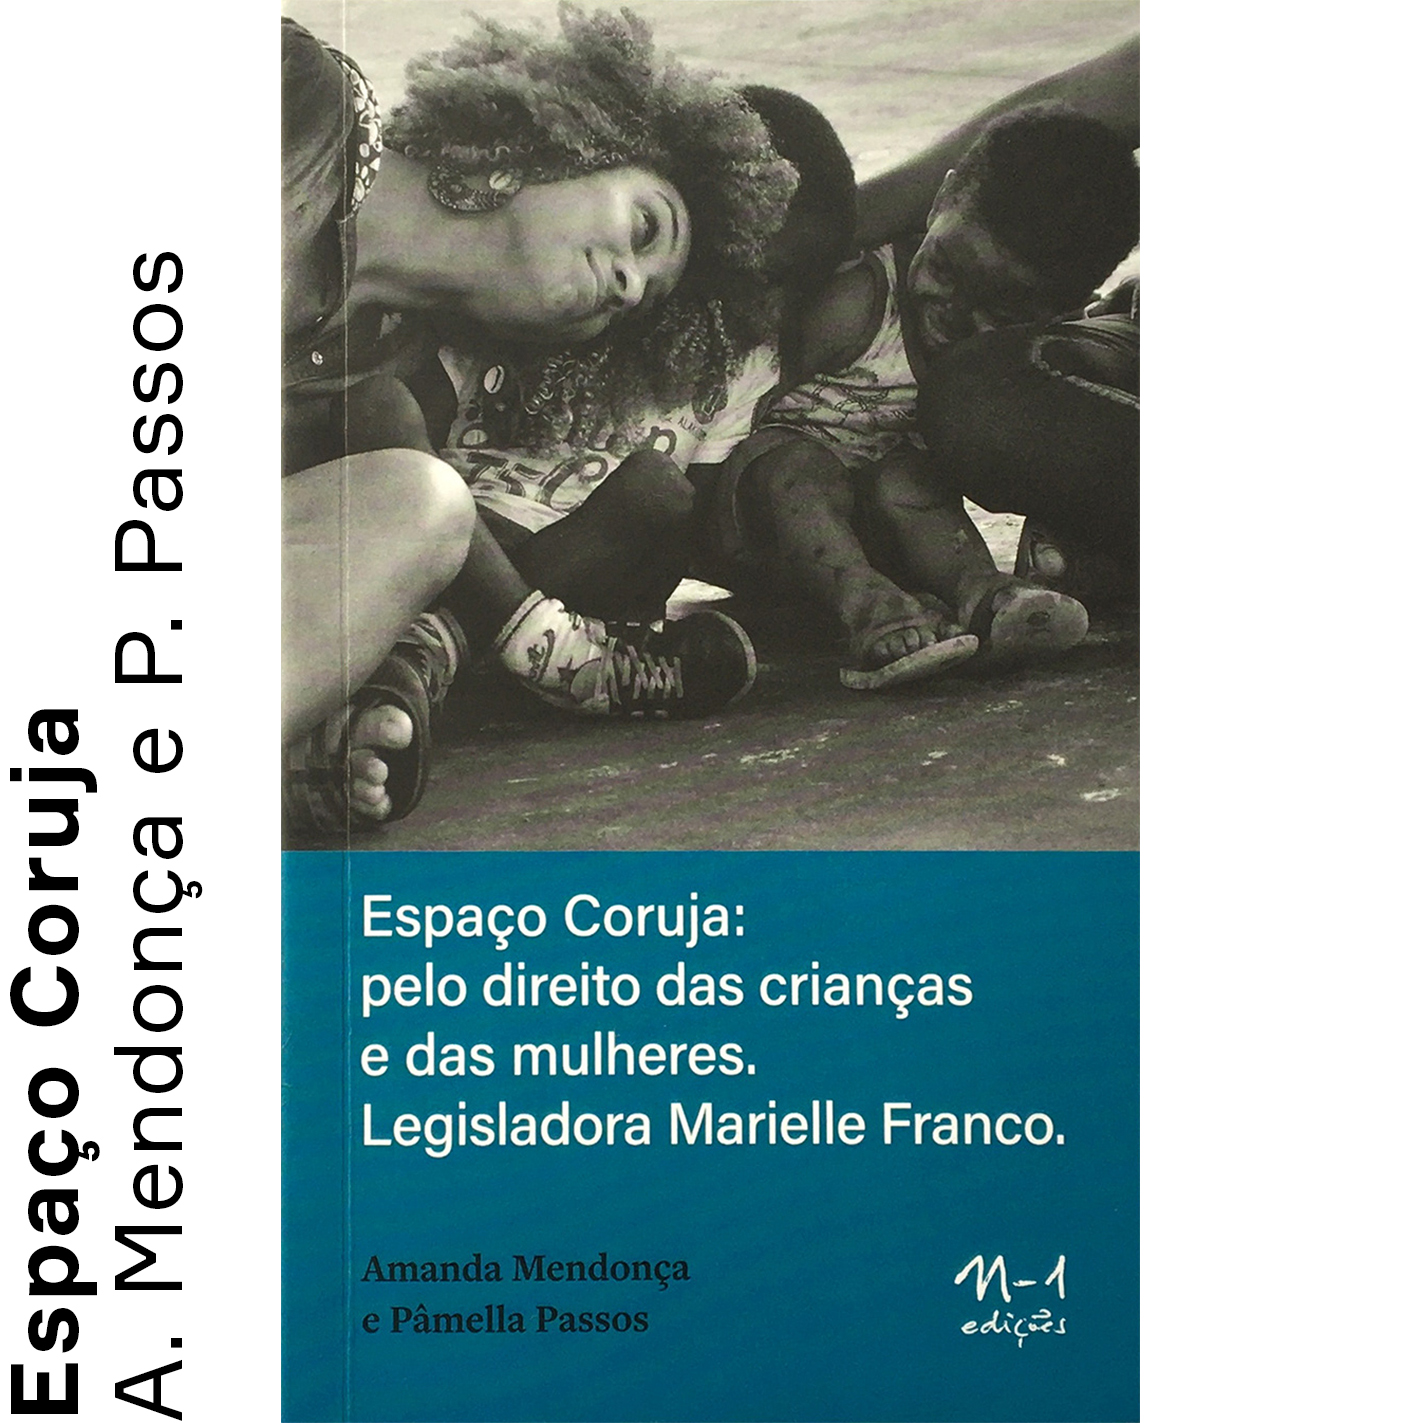
\includegraphics[width=40mm]{./grid2/coruja.jpg}}
\subfloat{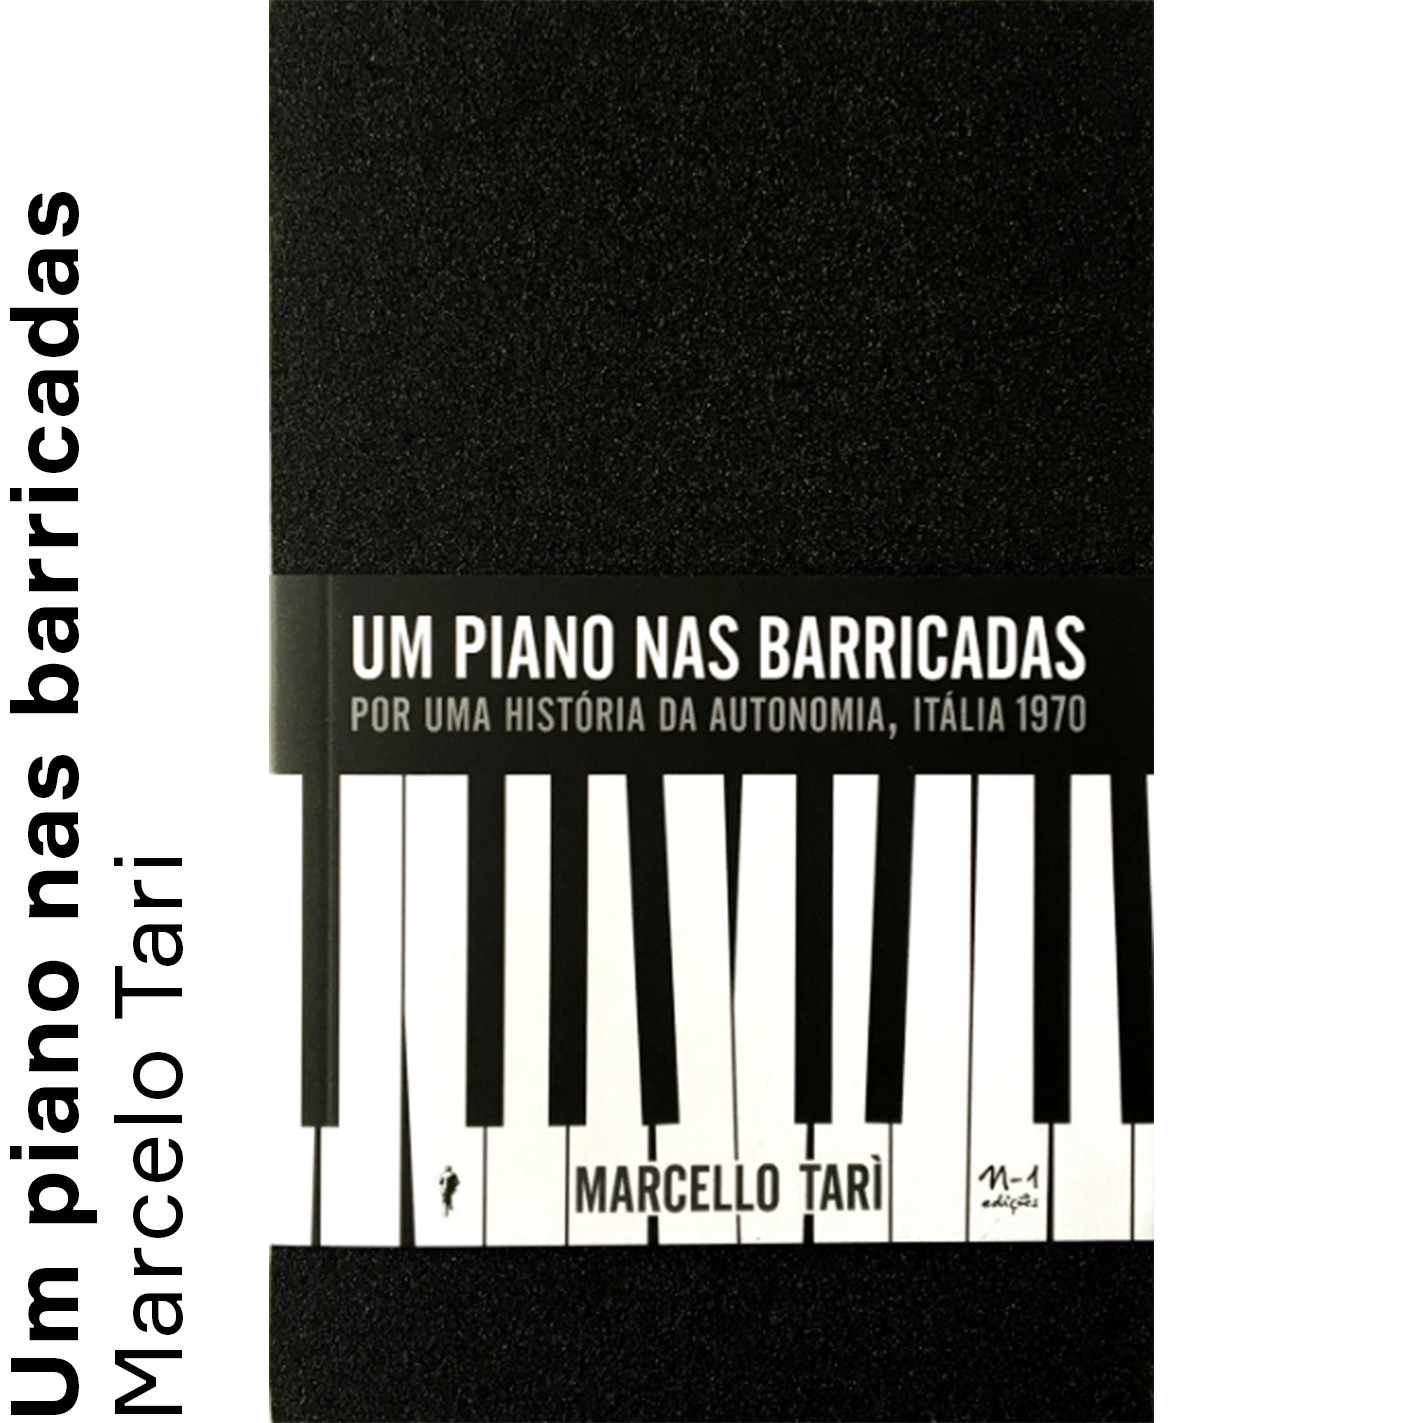
\includegraphics[width=40mm]{./grid2/barricada.jpg}}
\subfloat{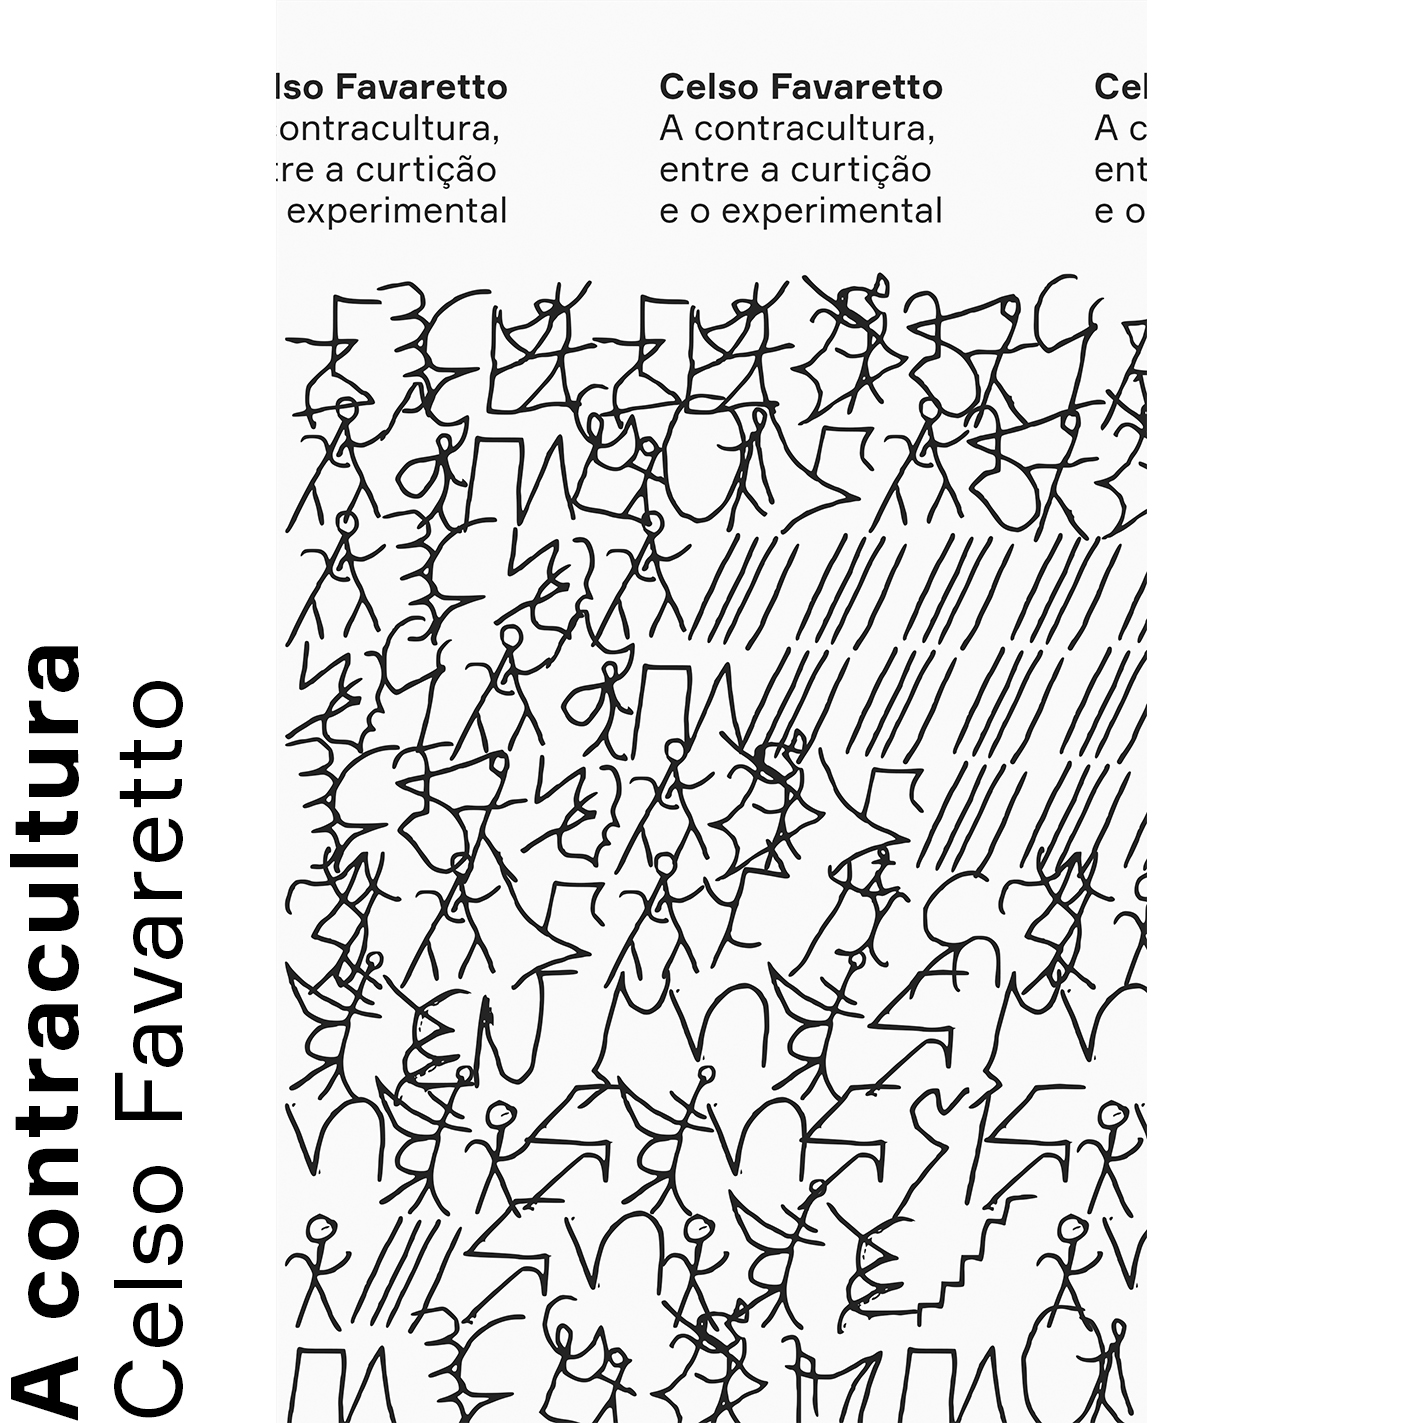
\includegraphics[width=40mm]{./grid2/favaretto.jpg}}\\\hspace*{-.5cm}
\vspace{.5cm}
\subfloat{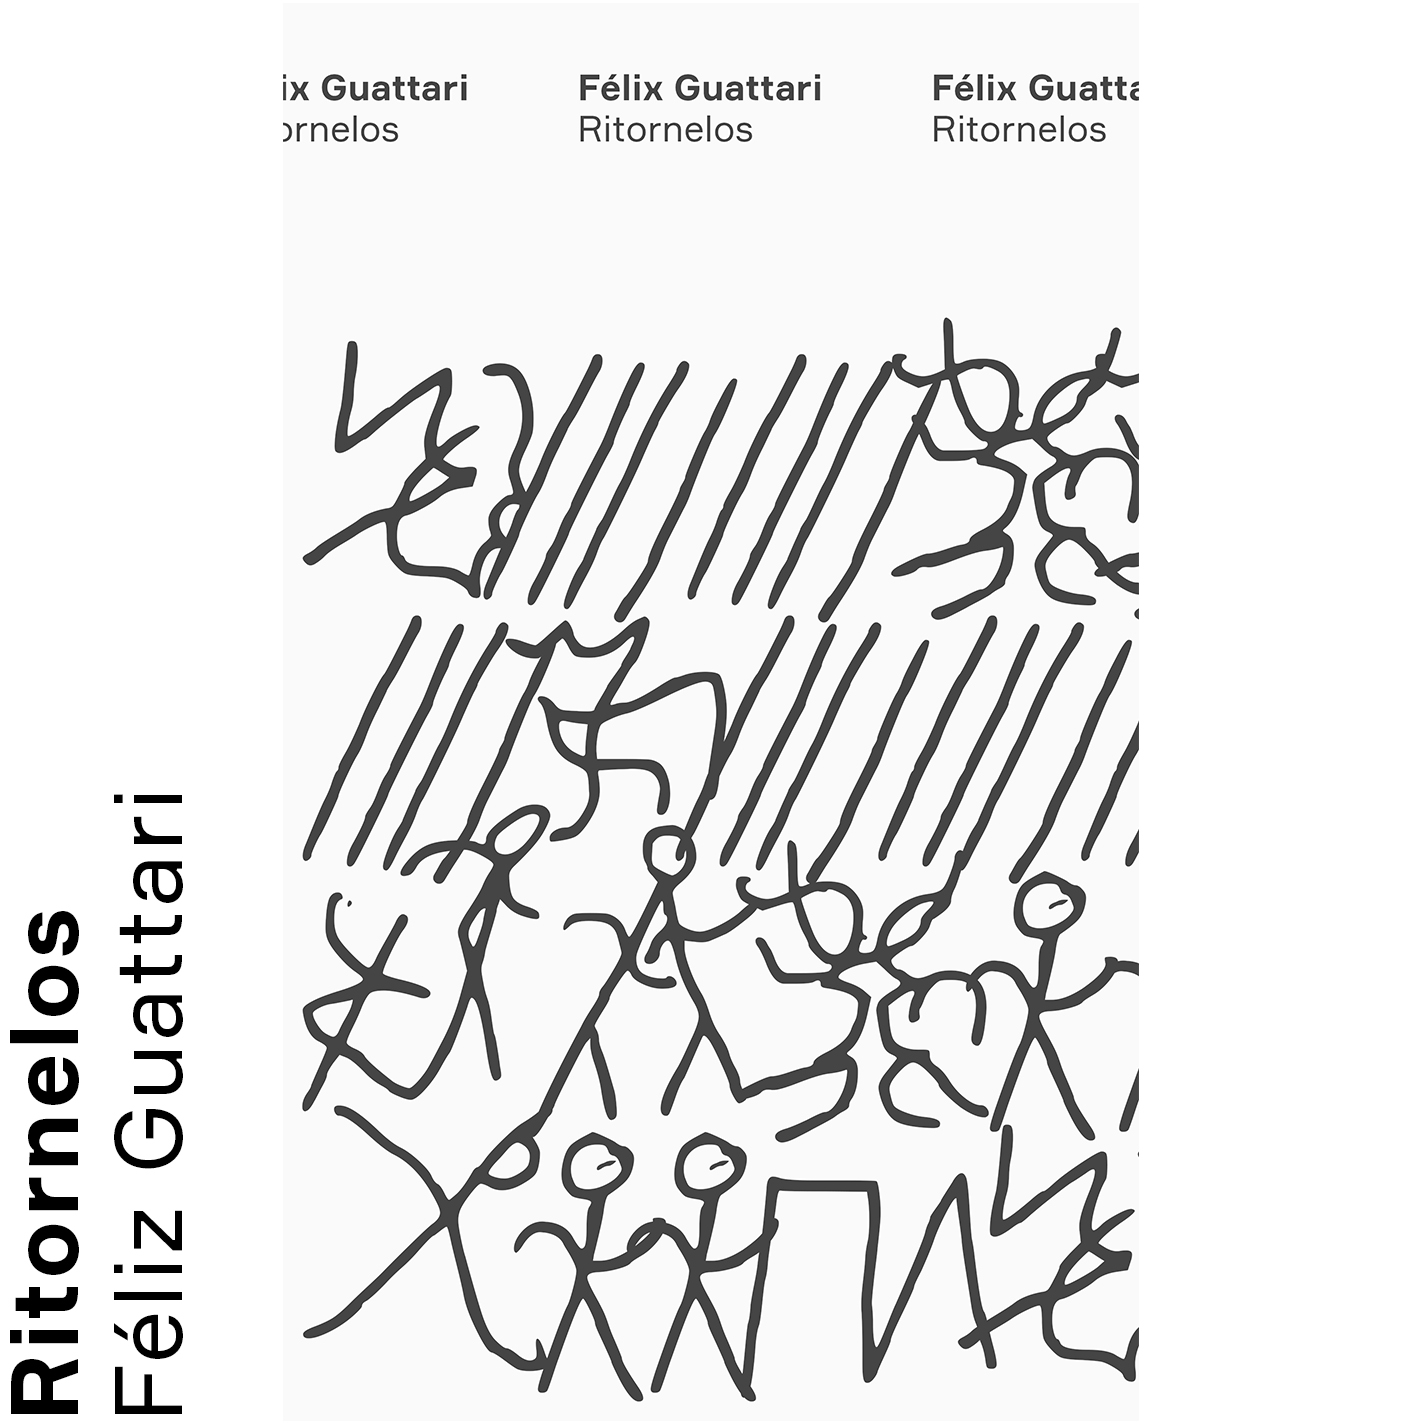
\includegraphics[width=40mm]{./grid2/guattari.jpg}}
\subfloat{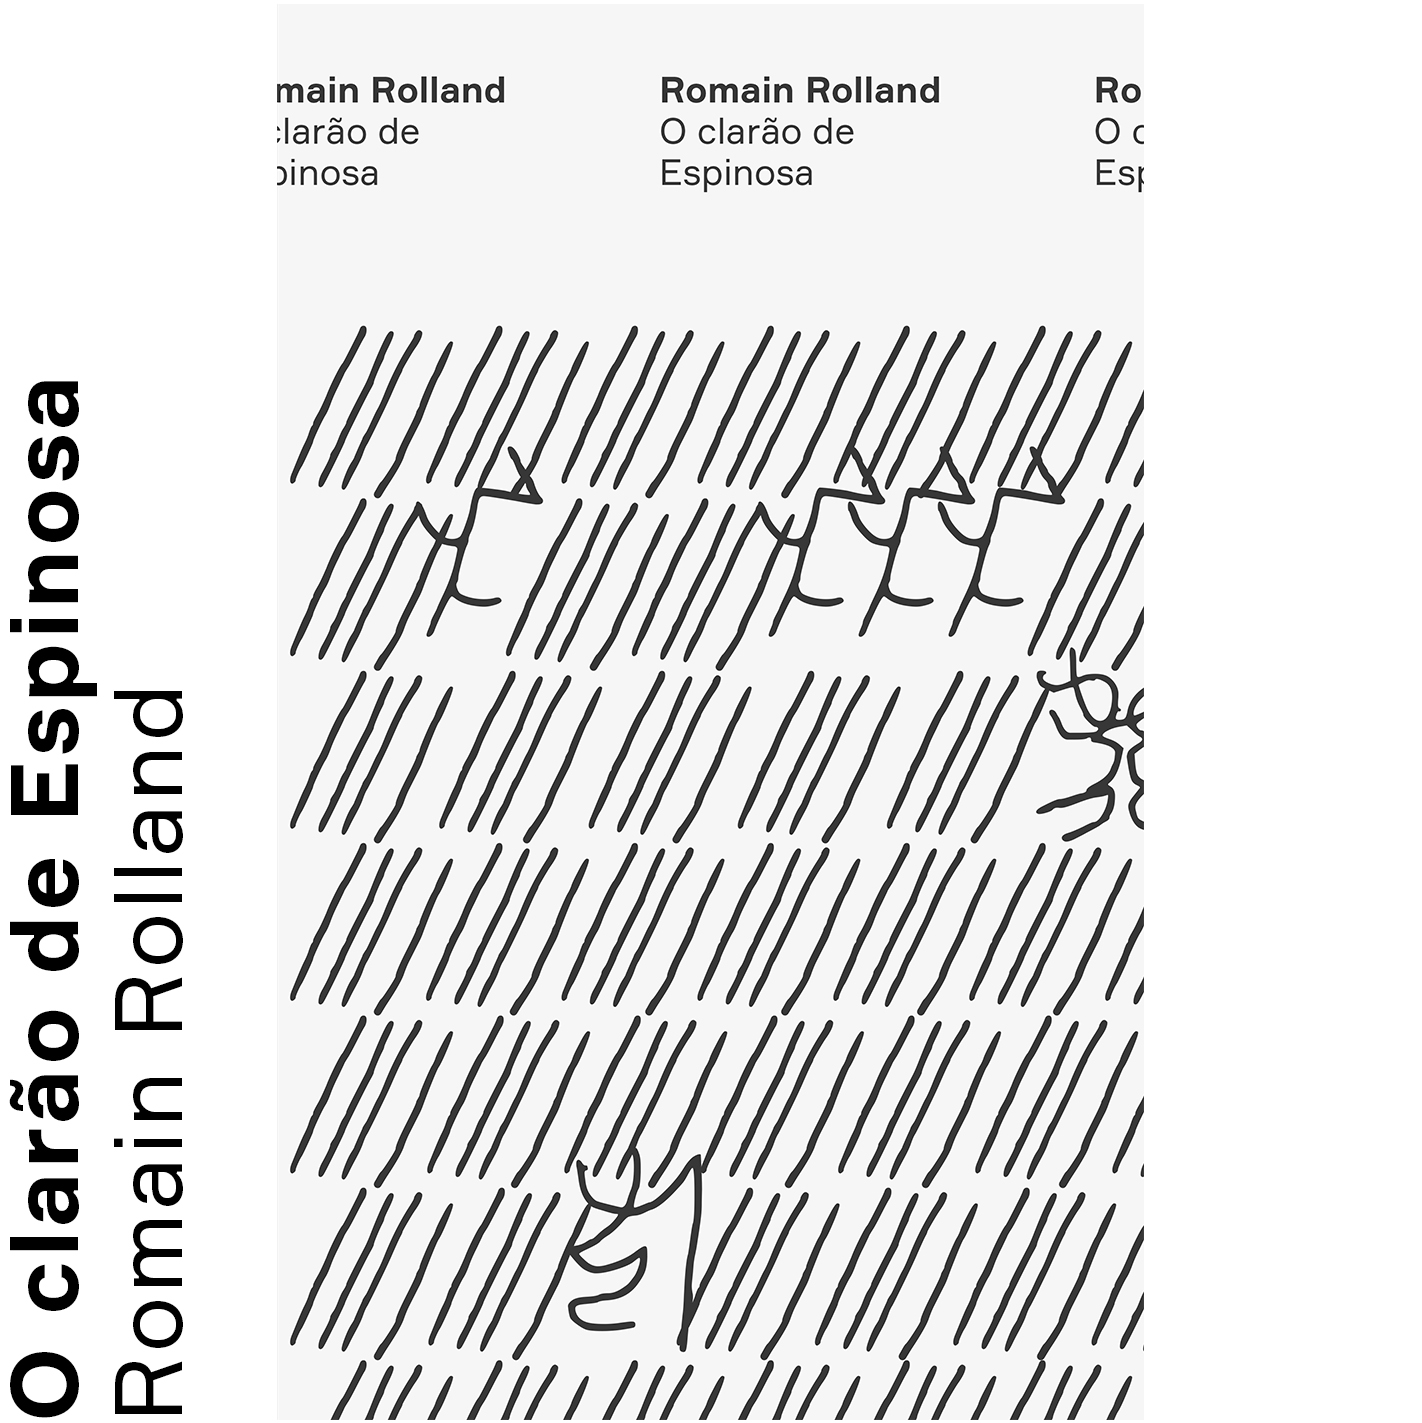
\includegraphics[width=40mm]{./grid2/rolland.jpg}}
\subfloat{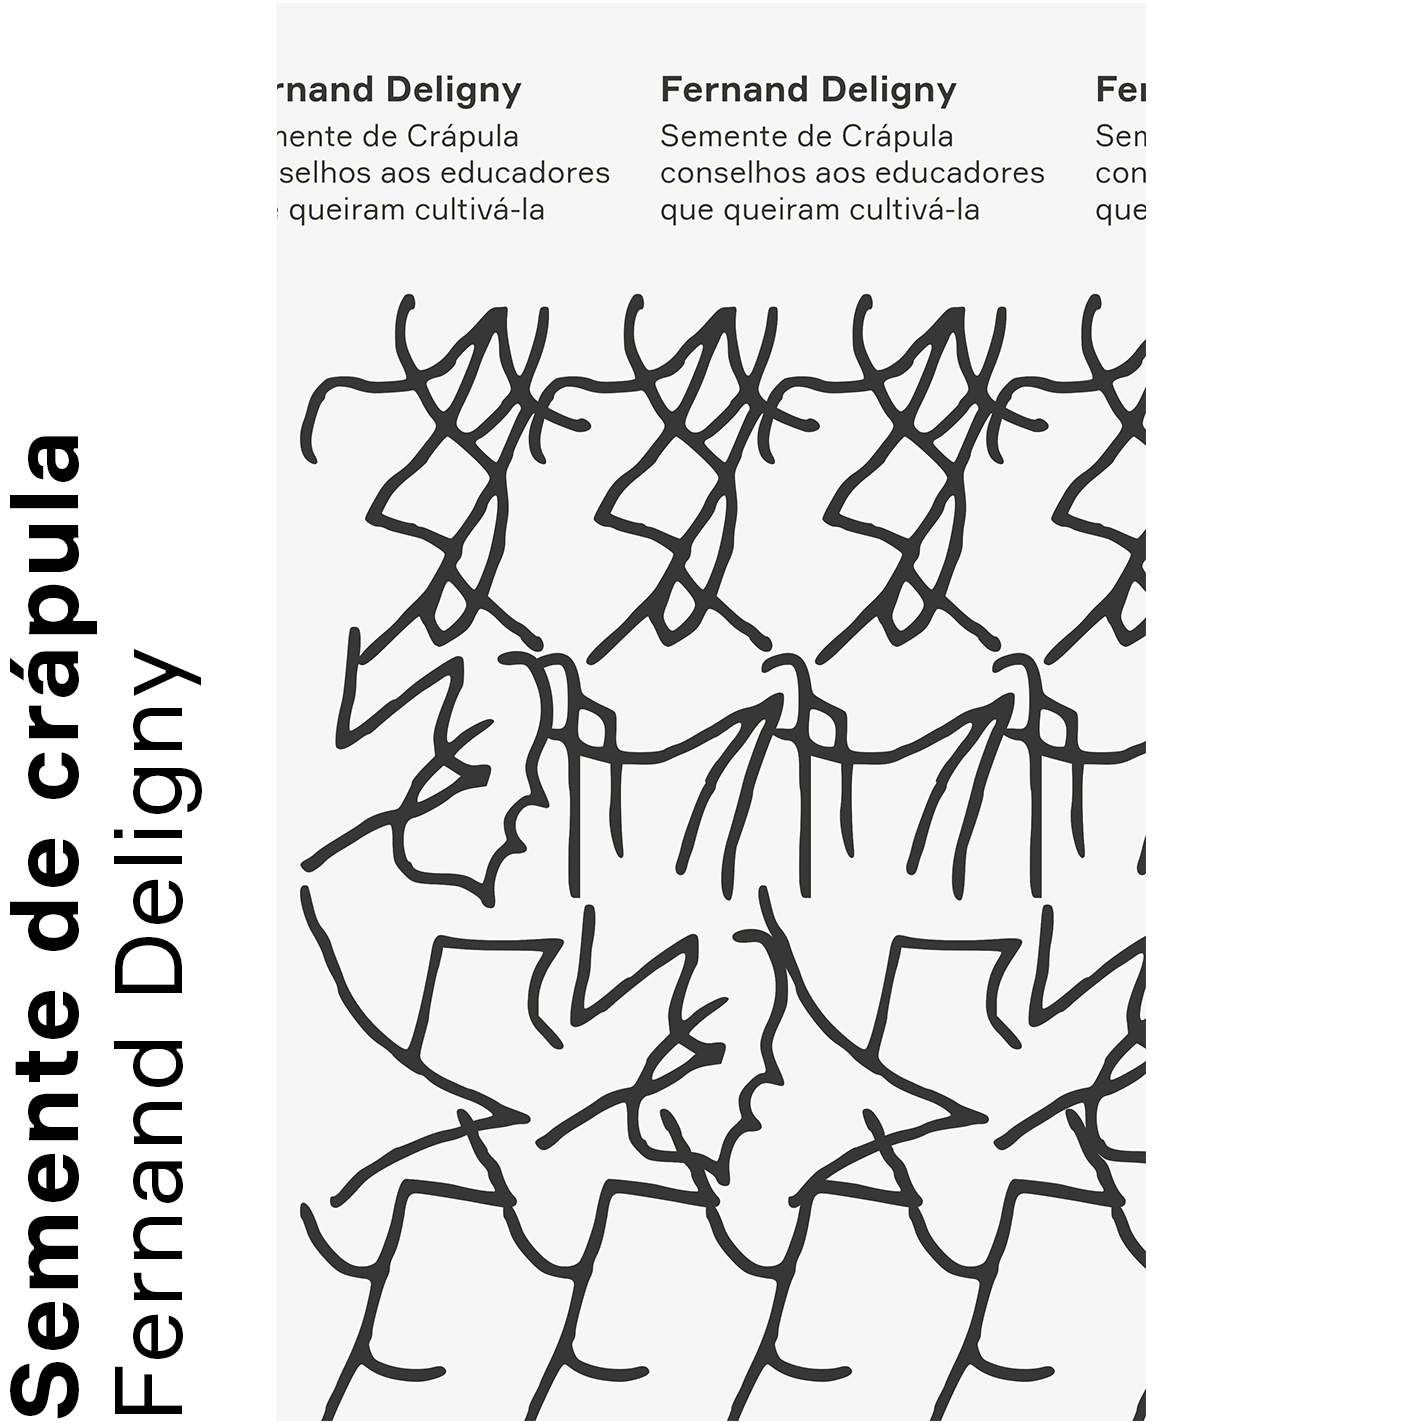
\includegraphics[width=40mm]{./grid2/deligny.jpg}}\\\hspace*{-.5cm}
\vspace{.5cm}
\subfloat{
\includegraphics[width=40mm]{./grid2/cover.jpg}}
\subfloat{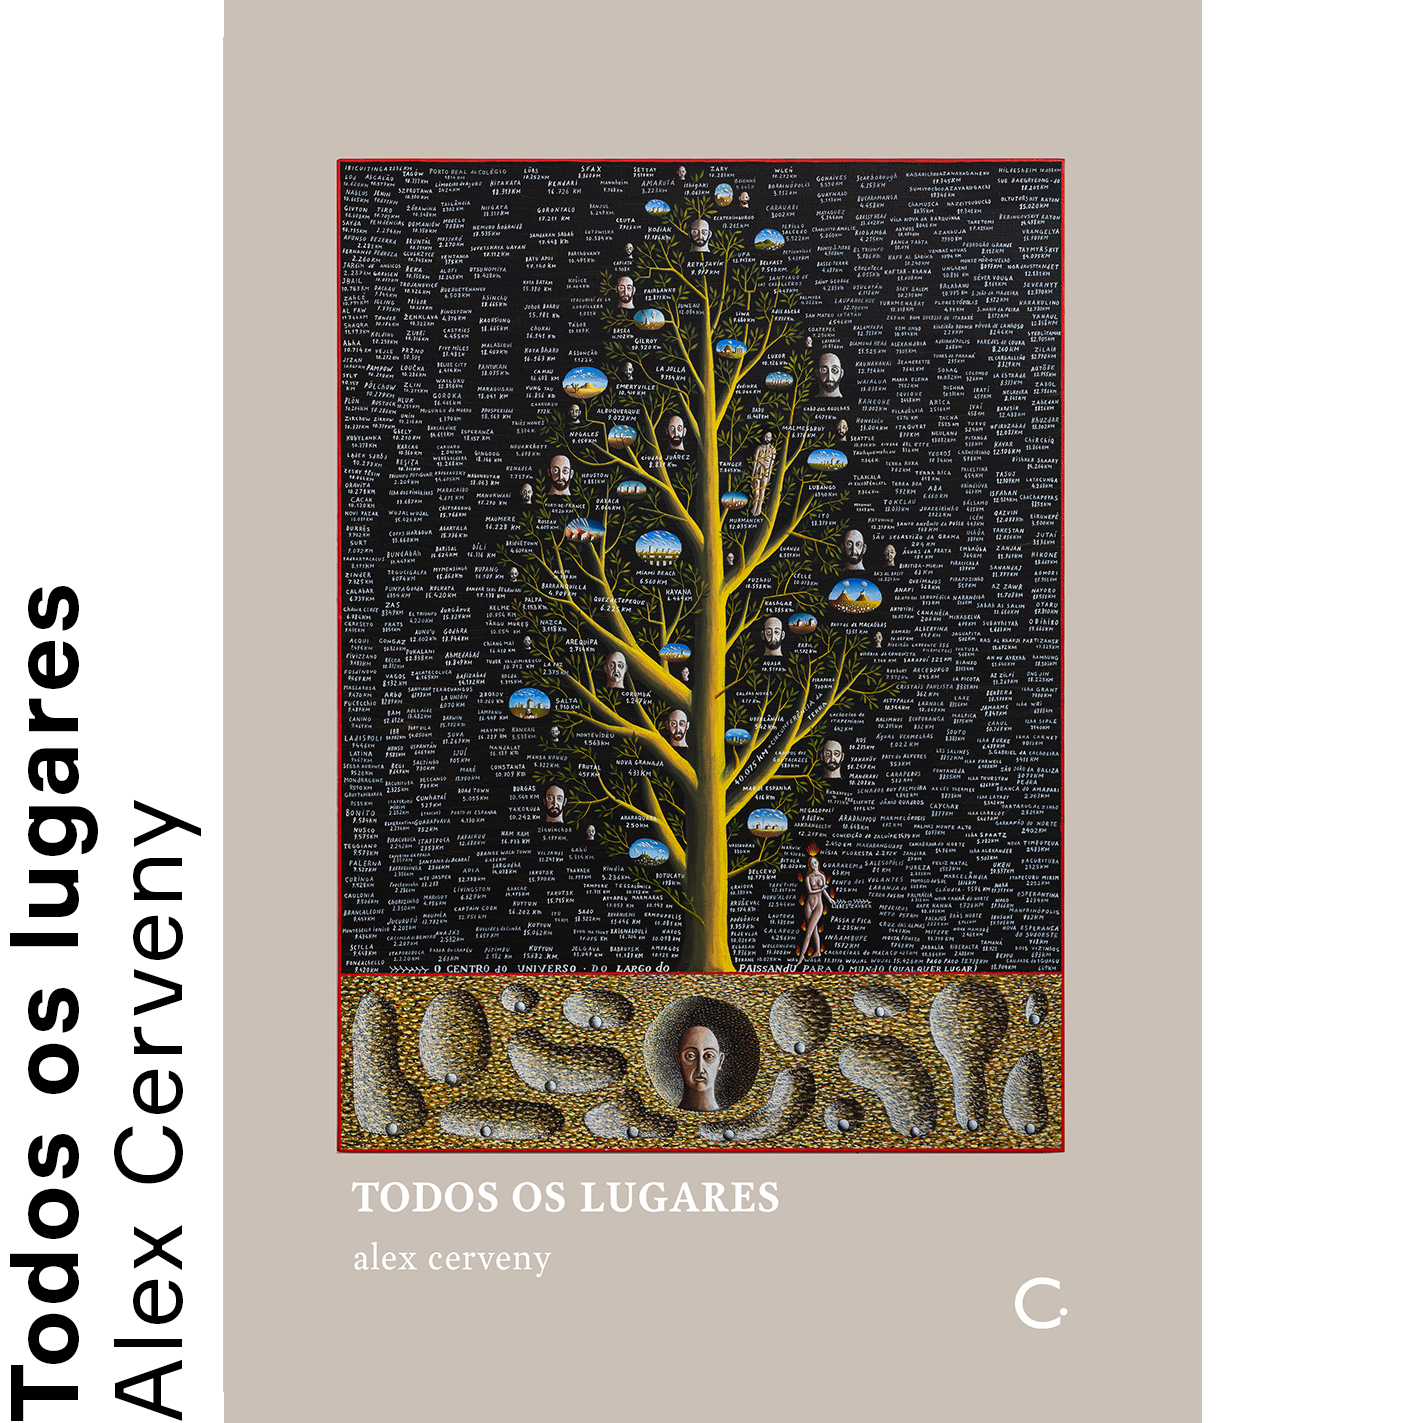
\includegraphics[width=40mm]{./grid2/lugares.jpg}}
\subfloat{
\includegraphics[width=40mm]{./grid2/antifa.jpg}}\\\hspace*{-.5cm}
\vspace{.5cm}
\subfloat{
\includegraphics[width=40mm]{./grid2/soma.jpg}}
\subfloat{
\includegraphics[width=40mm]{./grid2/black.jpg}}
\subfloat{
\includegraphics[width=40mm]{./grid2/1967.jpg}}\\
\end{tabular}
\end{figure}

\pagebreak

\begin{figure}[!htbp]
\begin{tabular}{cccc}

\vspace{.5cm}
\hspace*{-.5cm}
\subfloat{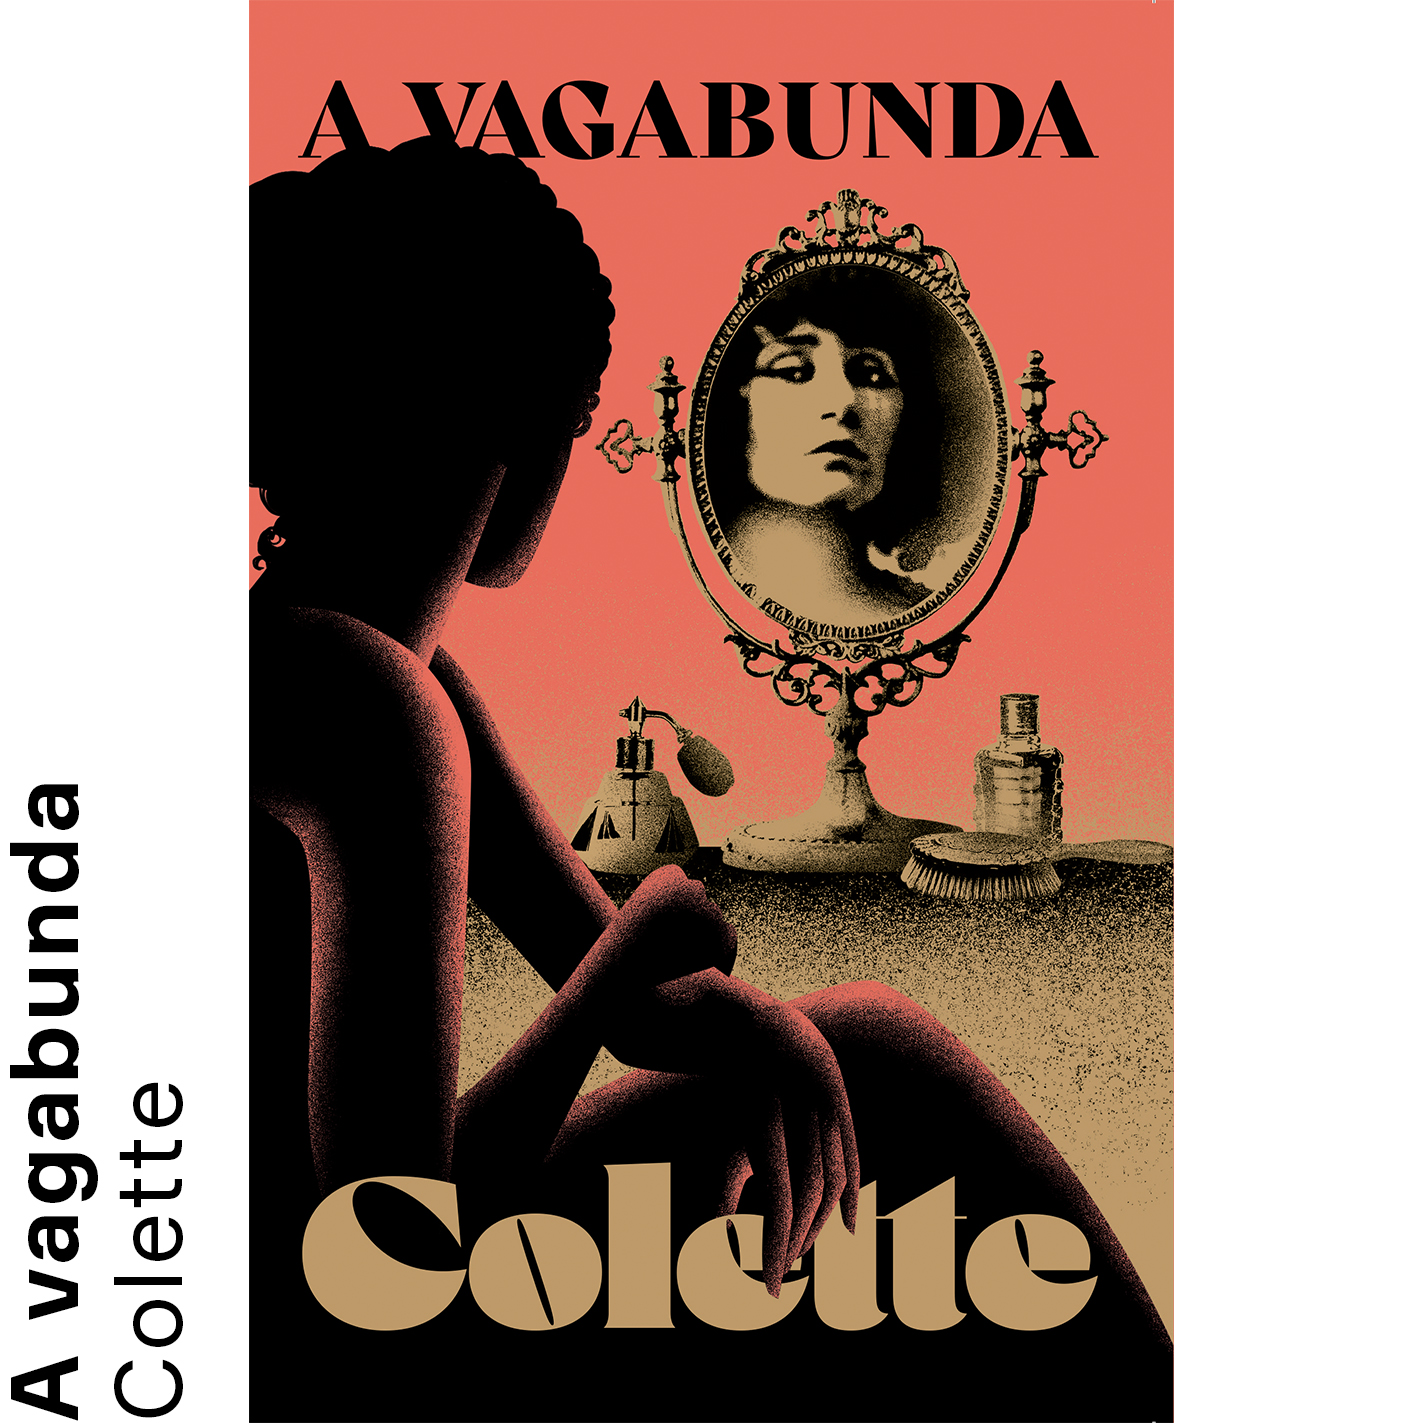
\includegraphics[width=40mm]{./grid2/vagabond.jpg}}
\subfloat{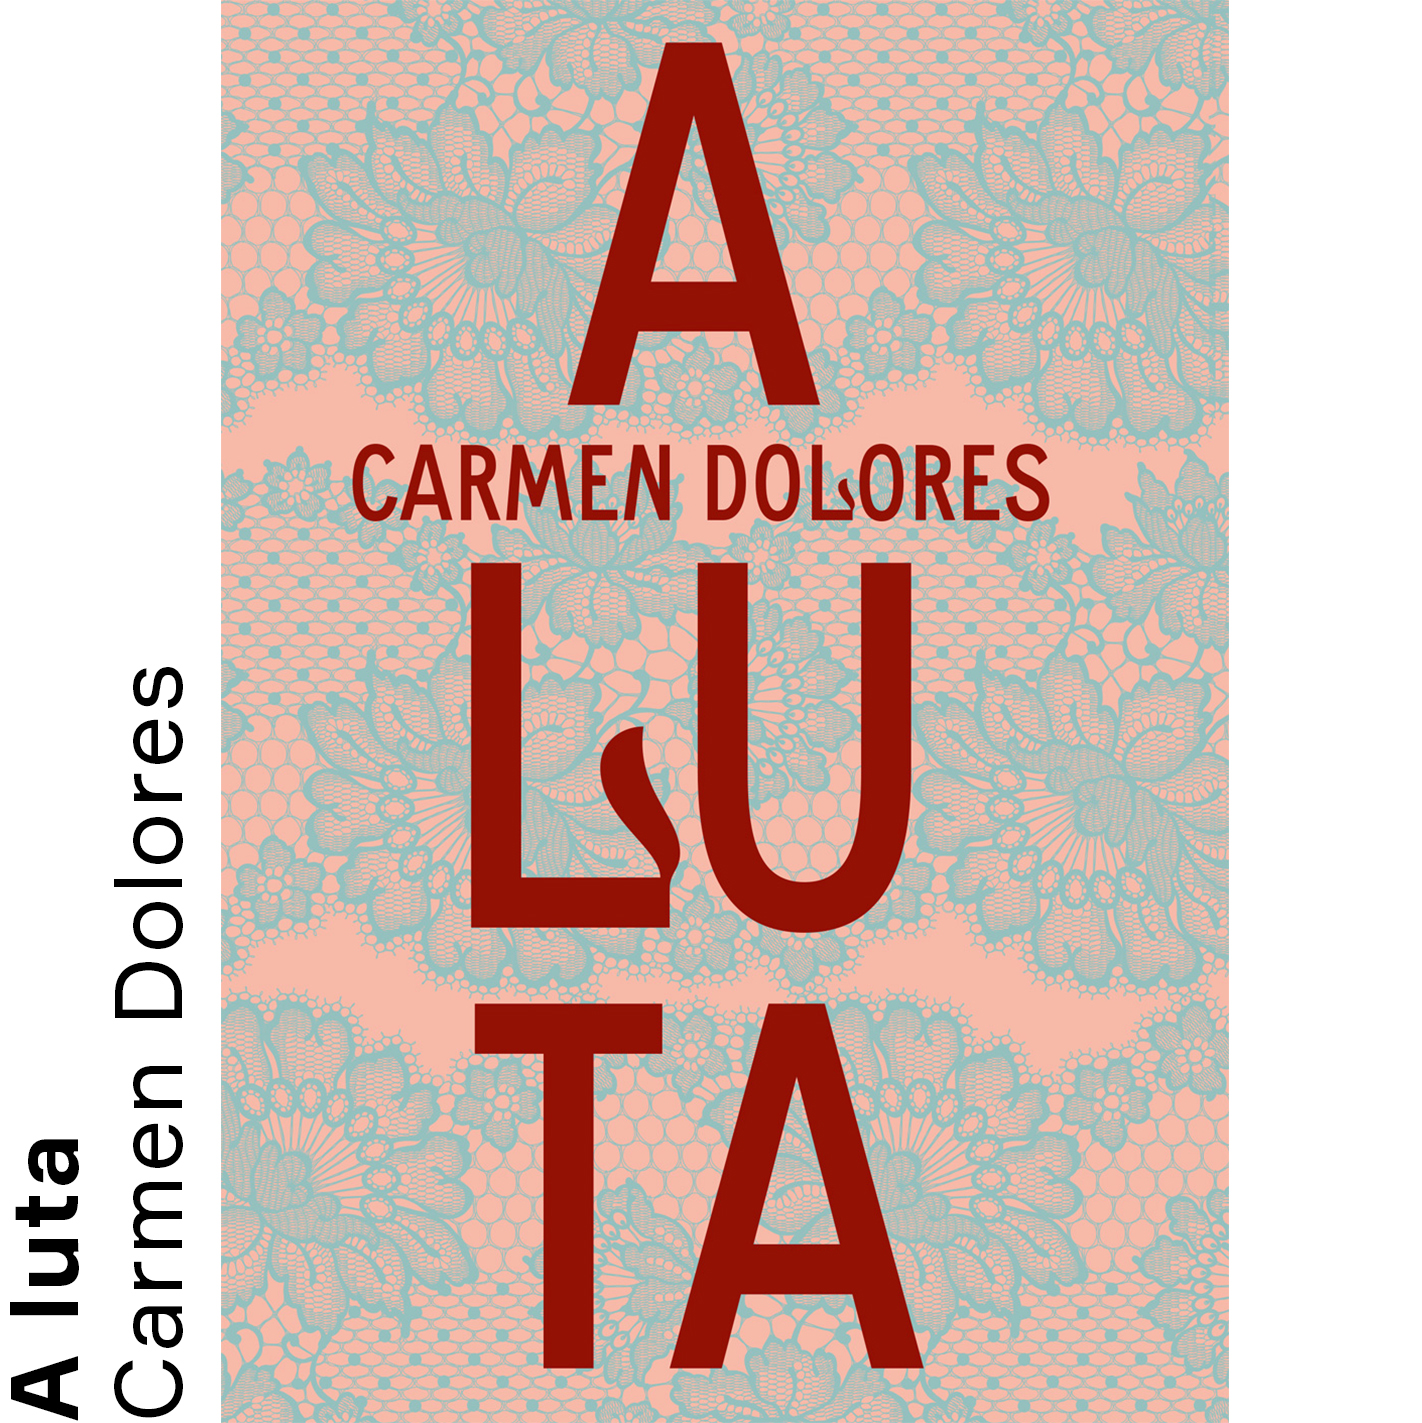
\includegraphics[width=40mm]{./grid2/luta.jpg}}
\subfloat{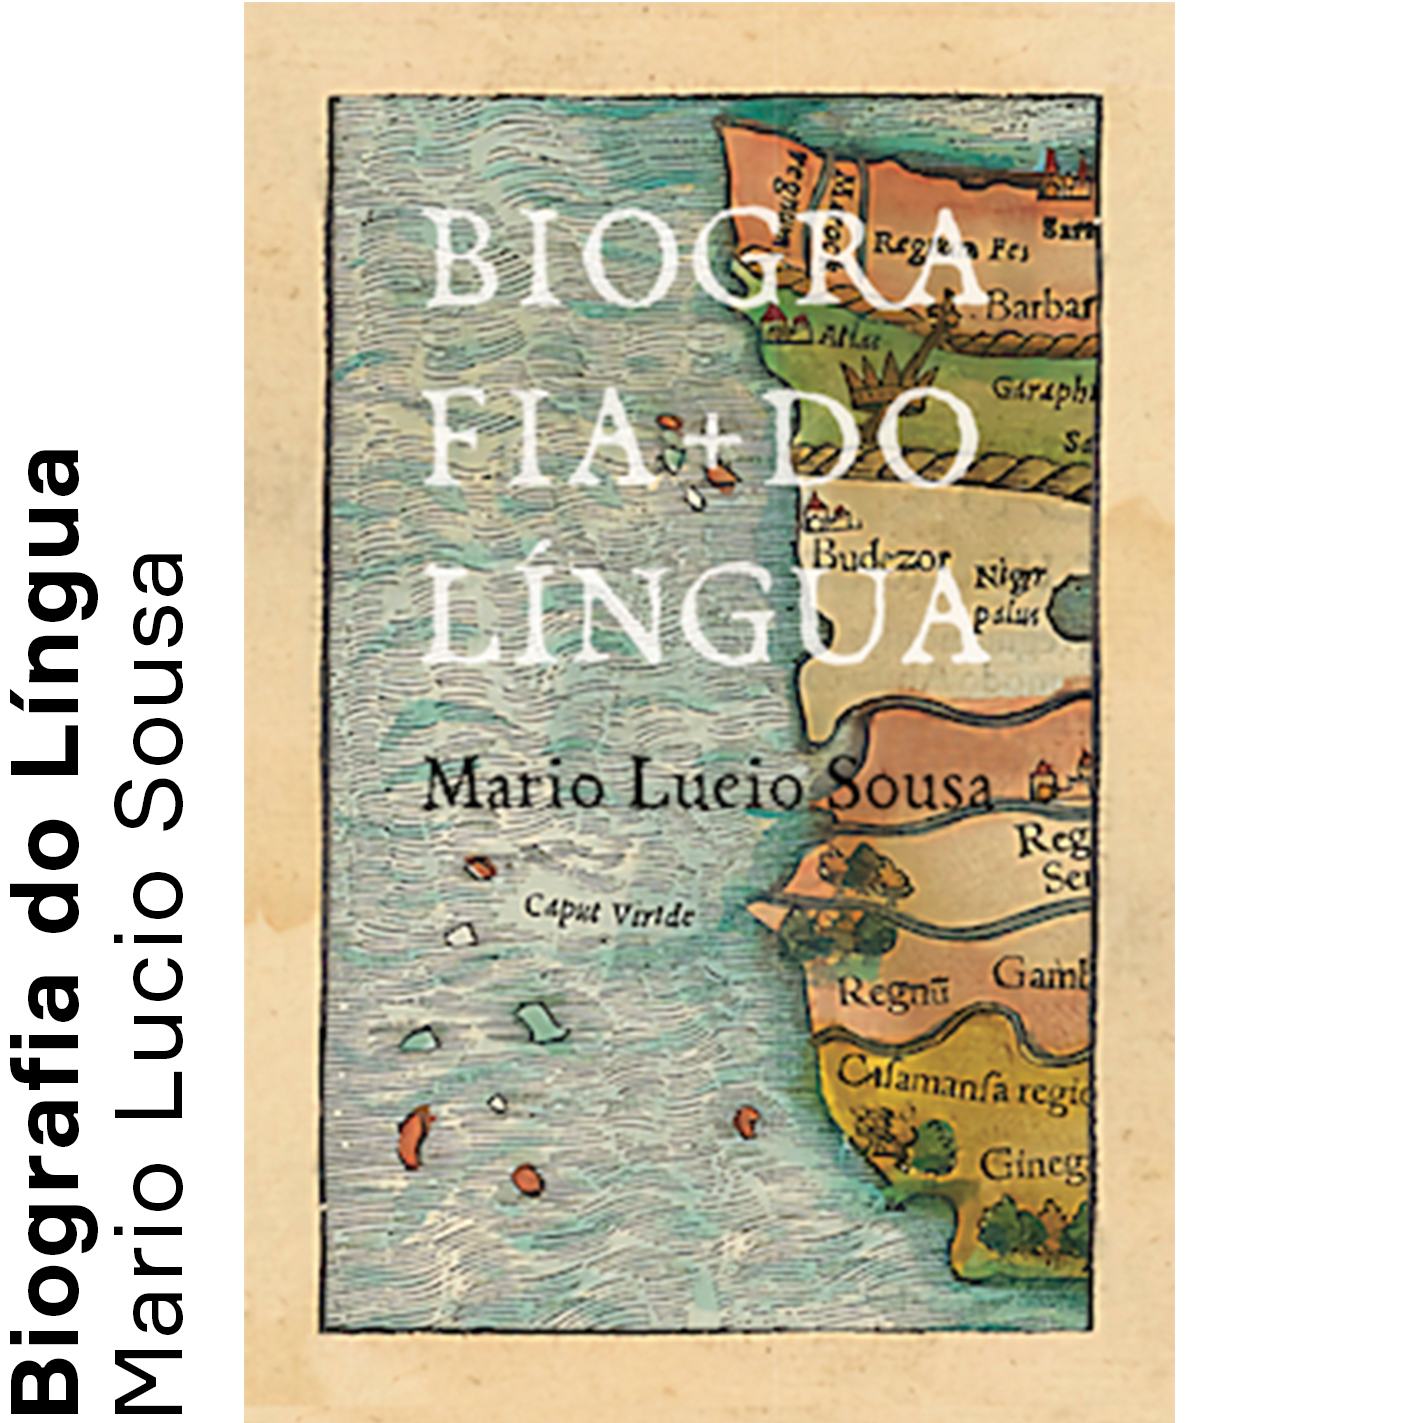
\includegraphics[width=40mm]{./grid2/lingua.jpg}}\\\hspace*{-.5cm}
\vspace{.5cm}
\subfloat{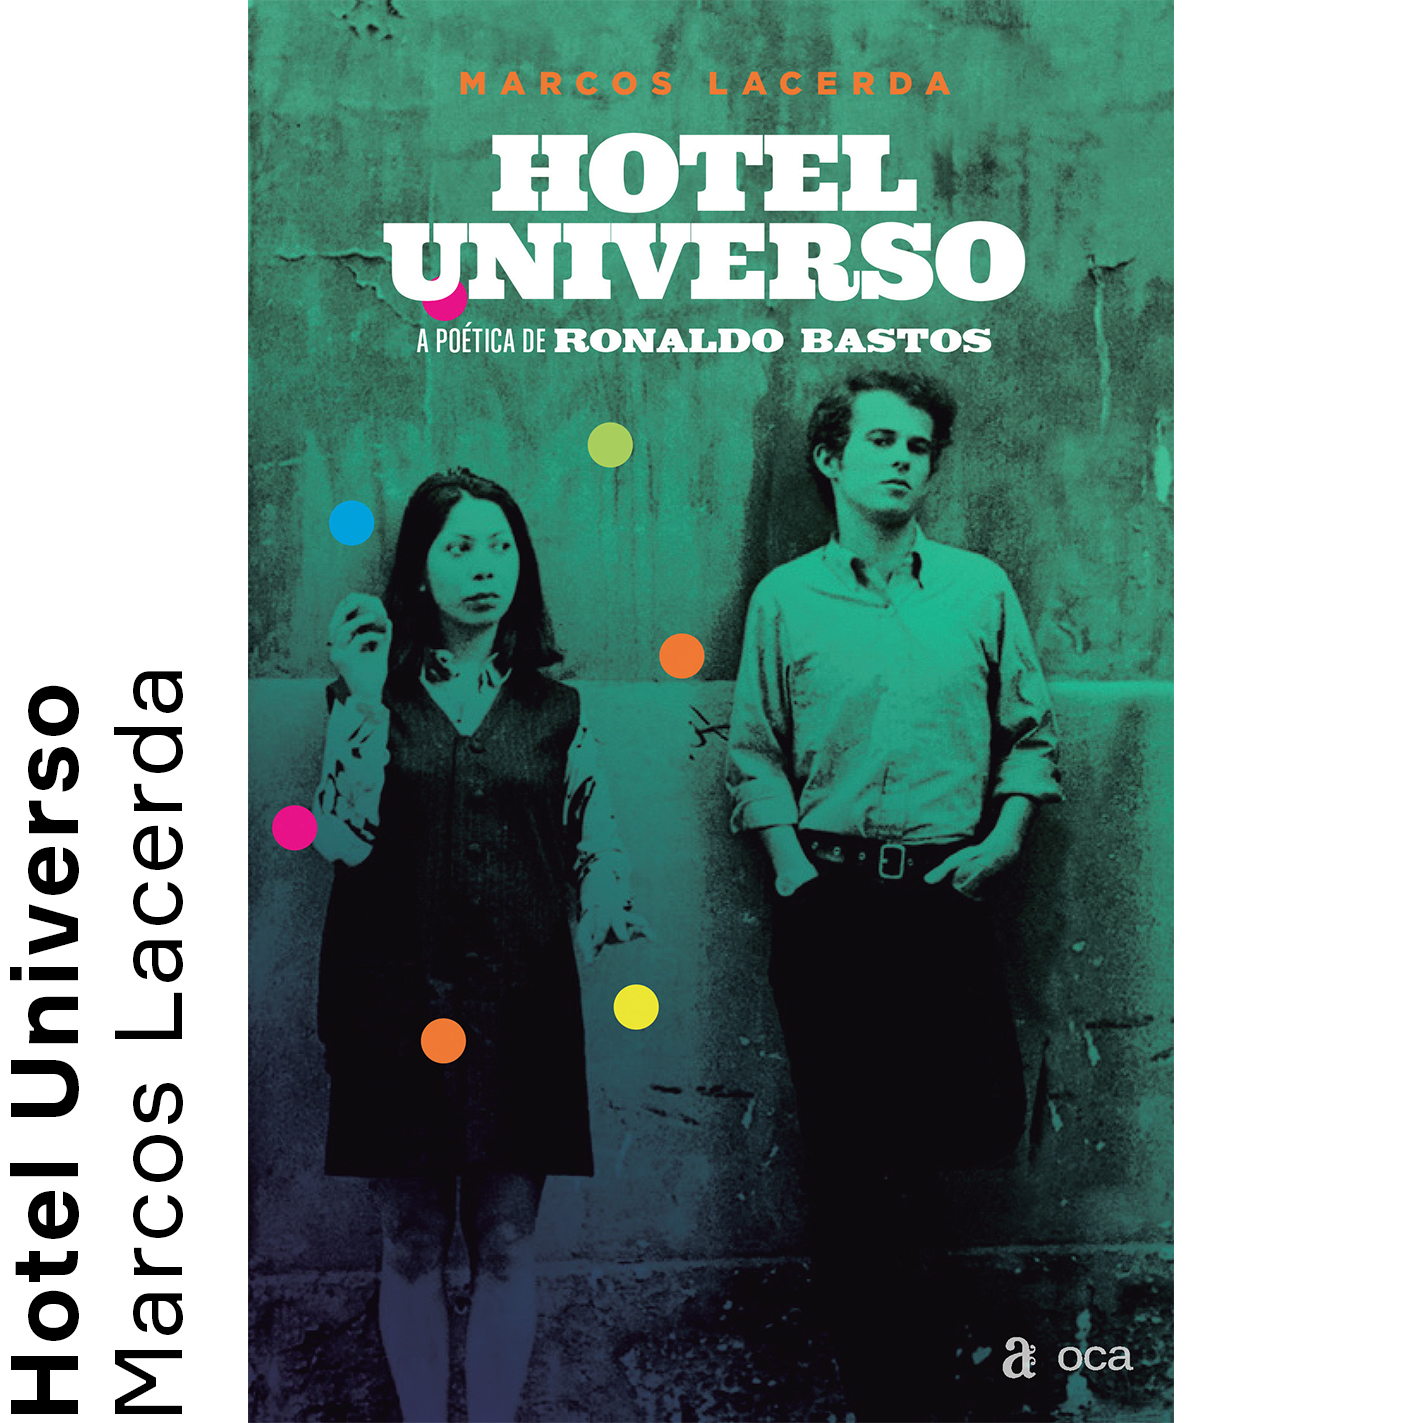
\includegraphics[width=40mm]{./grid2/hotel.jpg}}
\subfloat{
\includegraphics[width=40mm]{./grid2/tembeta.jpg}}
\subfloat{
\includegraphics[width=40mm]{./grid2/mautner.jpg}}\\\hspace*{-.5cm}
\vspace{.5cm}
\subfloat{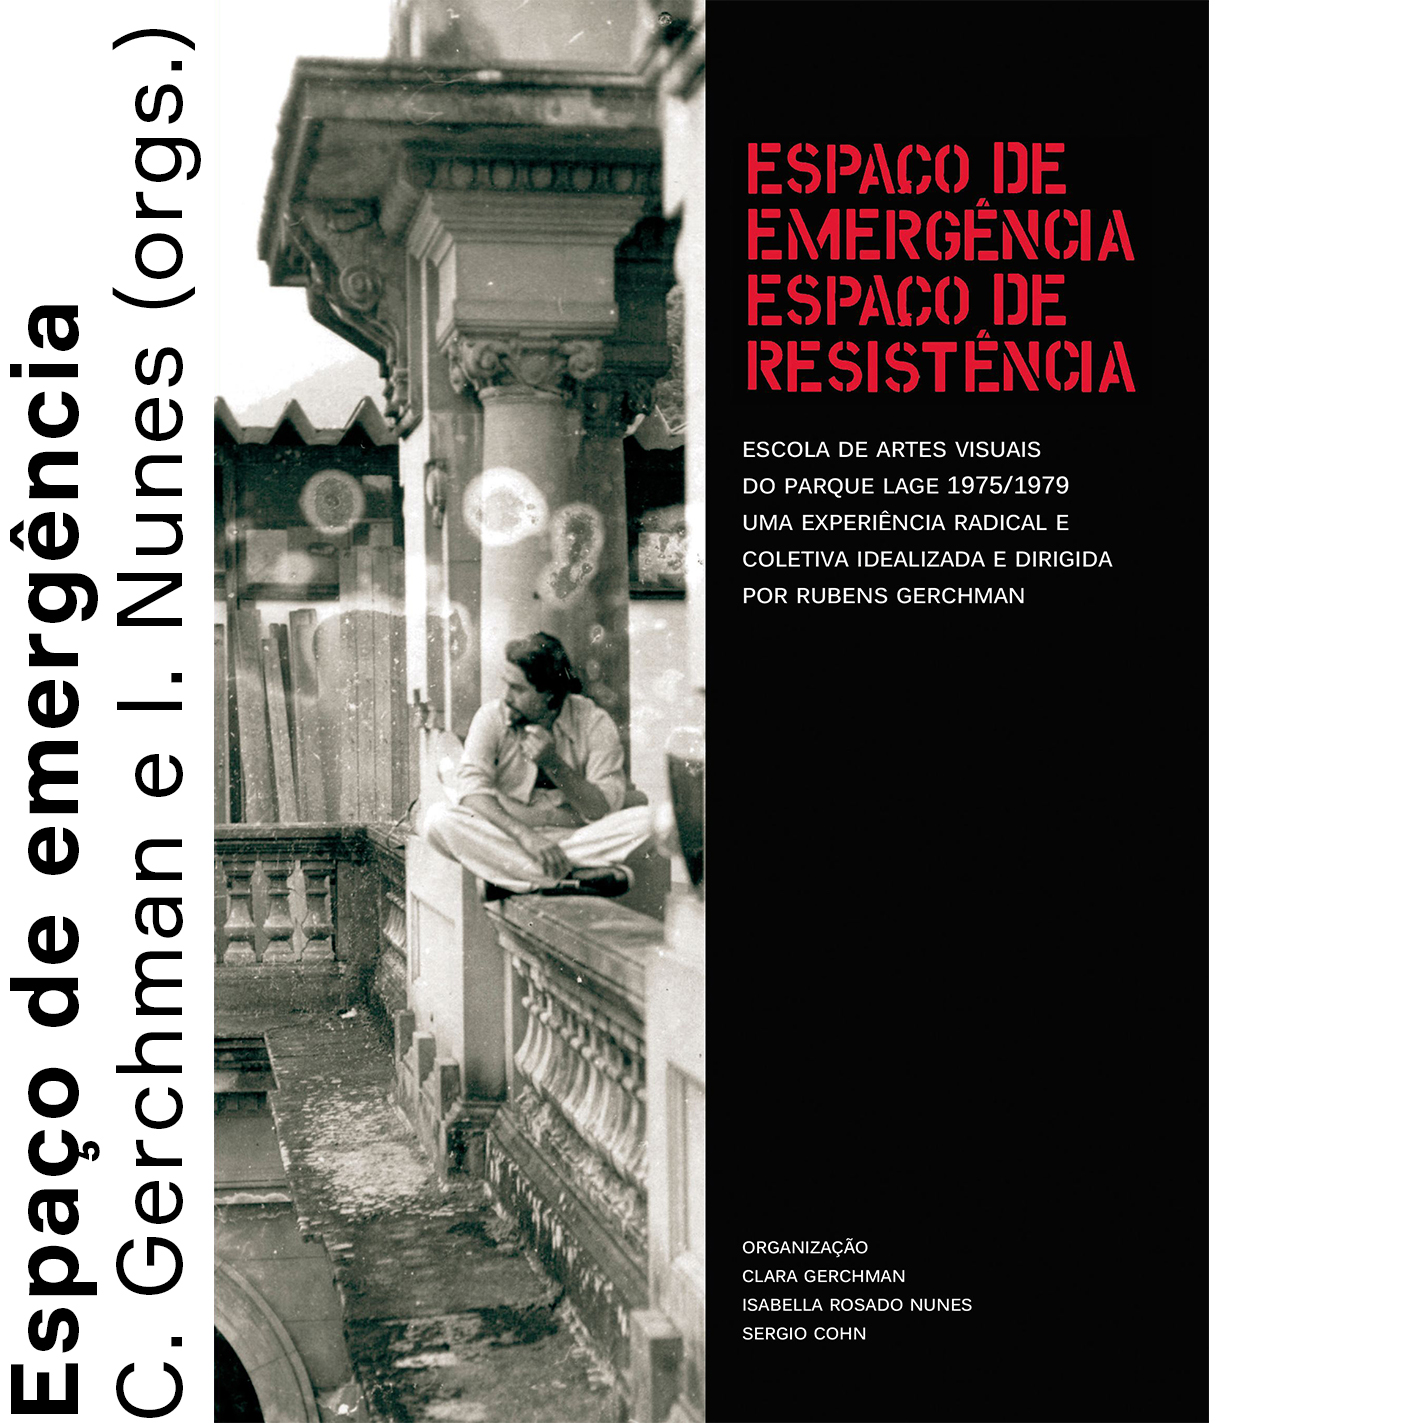
\includegraphics[width=40mm]{./grid2/lage.jpg}}
\subfloat{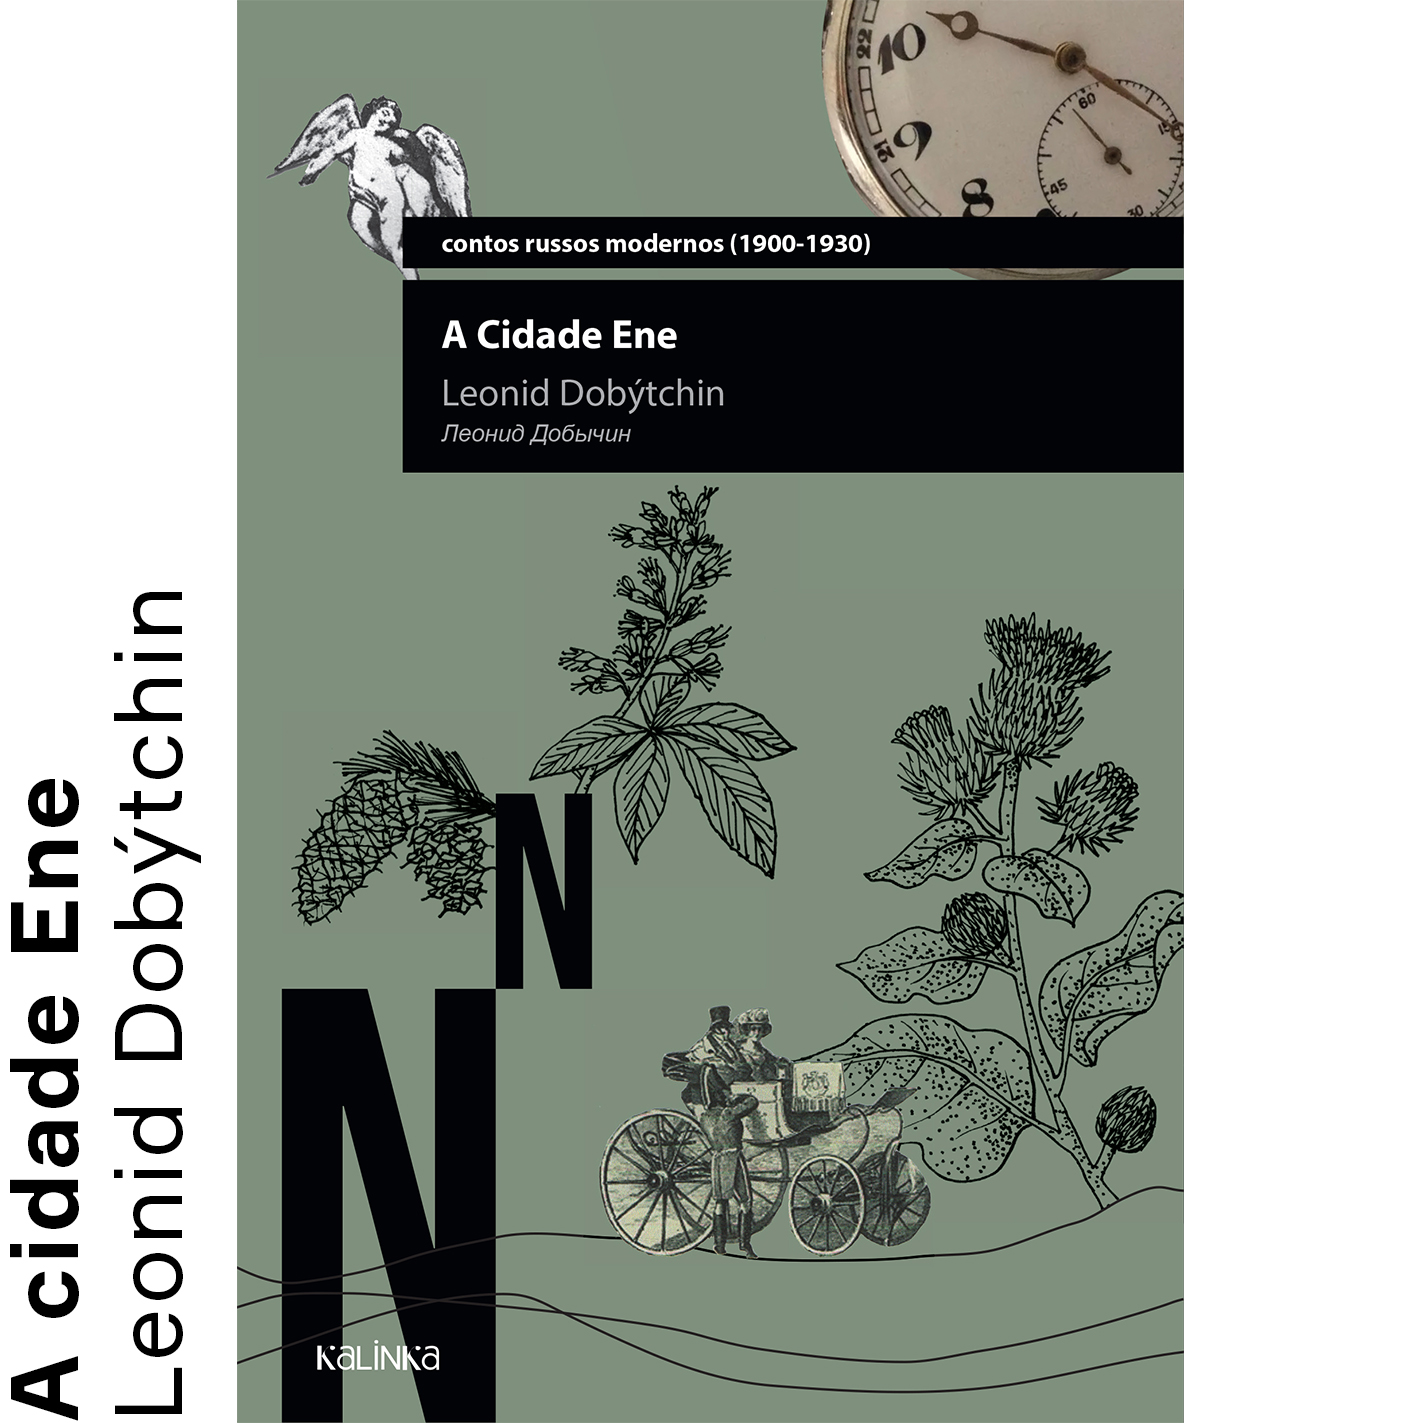
\includegraphics[width=40mm]{./grid2/cidaden.jpg}}
\subfloat{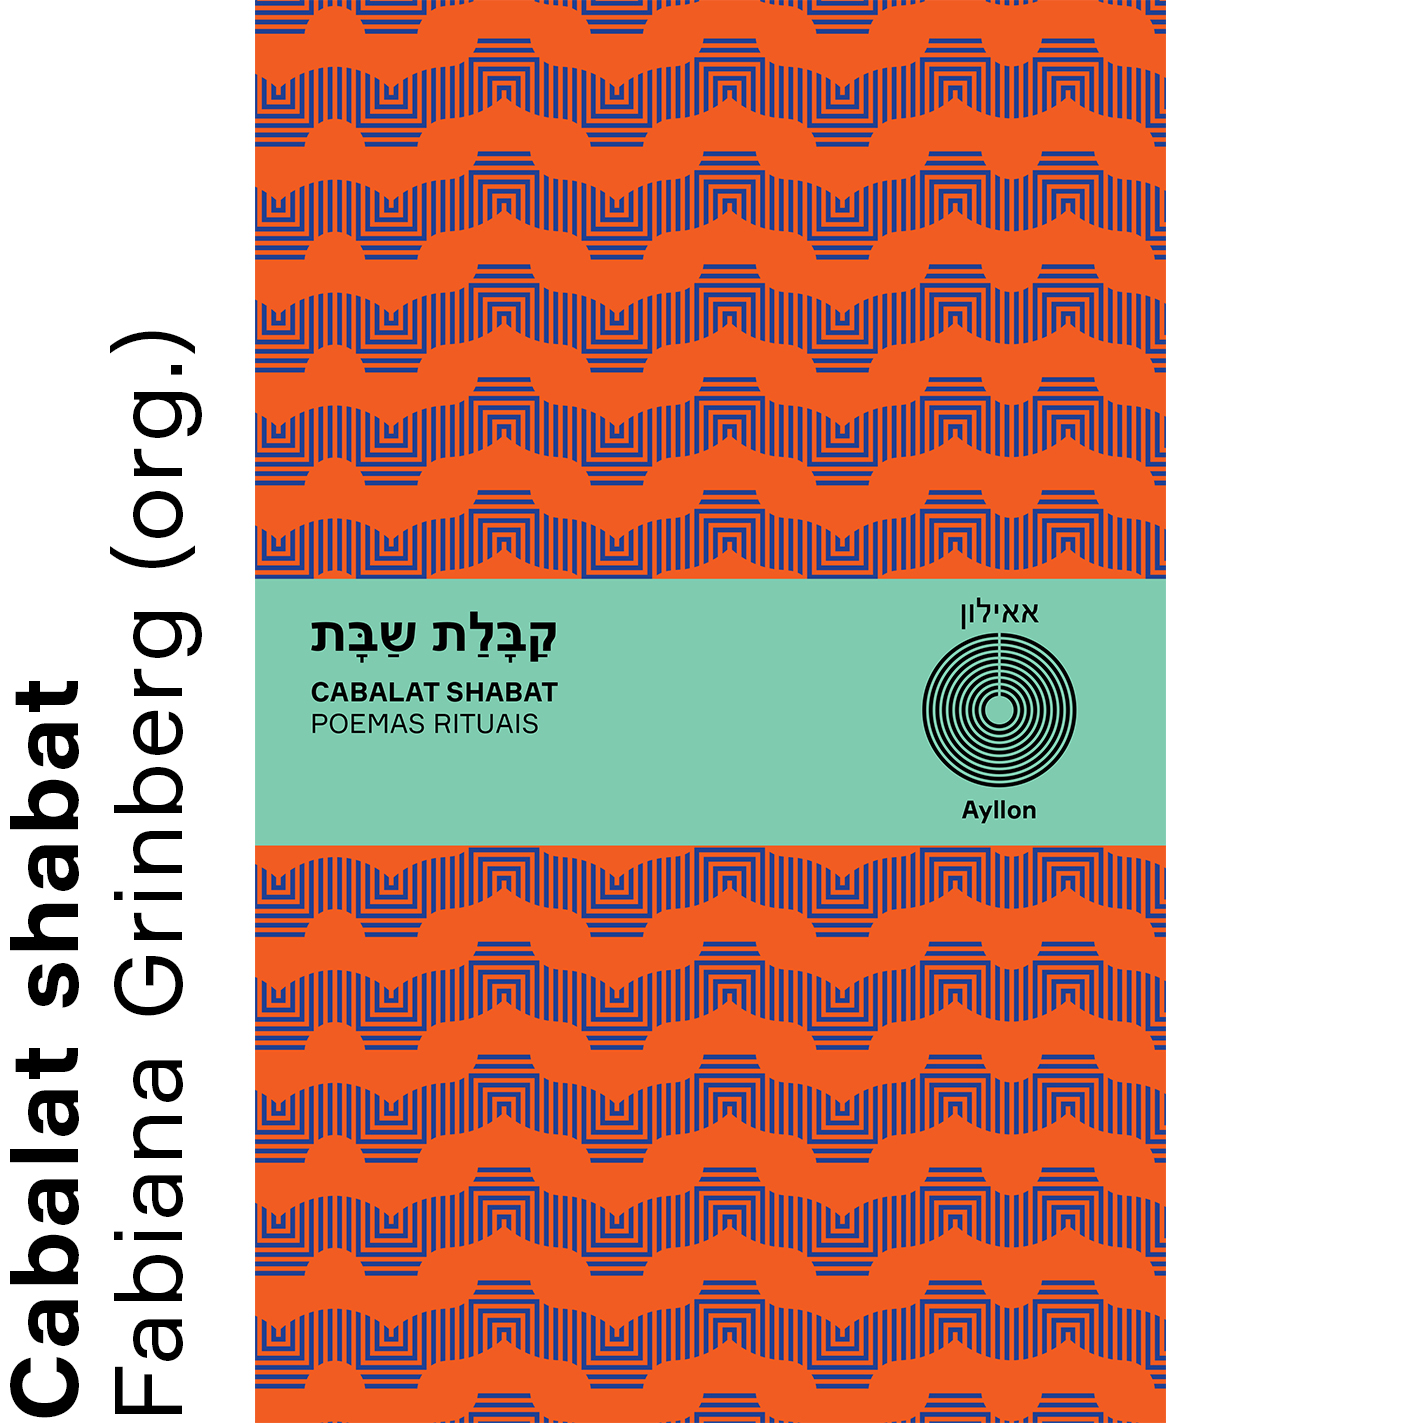
\includegraphics[width=40mm]{./grid2/cabalat.jpg}}\\\hspace*{-.5cm}
\vspace{.5cm}
\subfloat{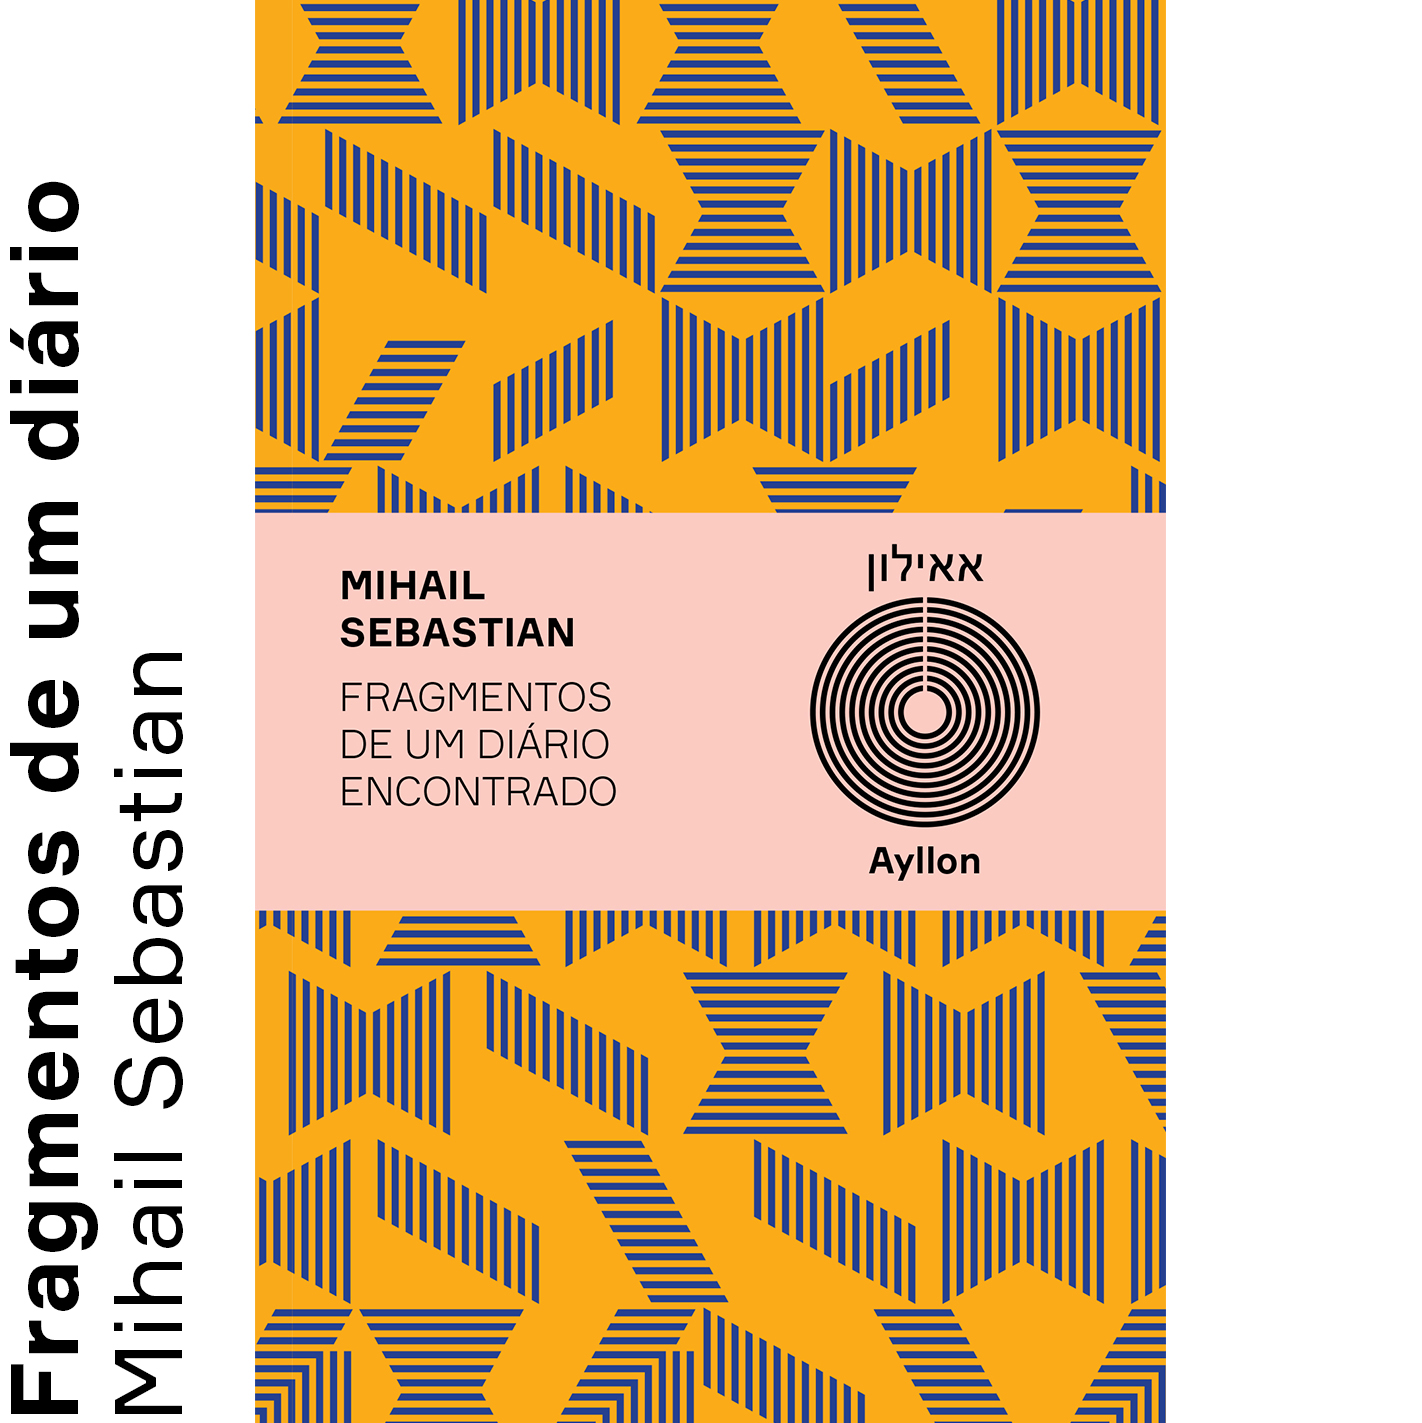
\includegraphics[width=40mm]{./grid2/sebastian.jpg}}
\subfloat{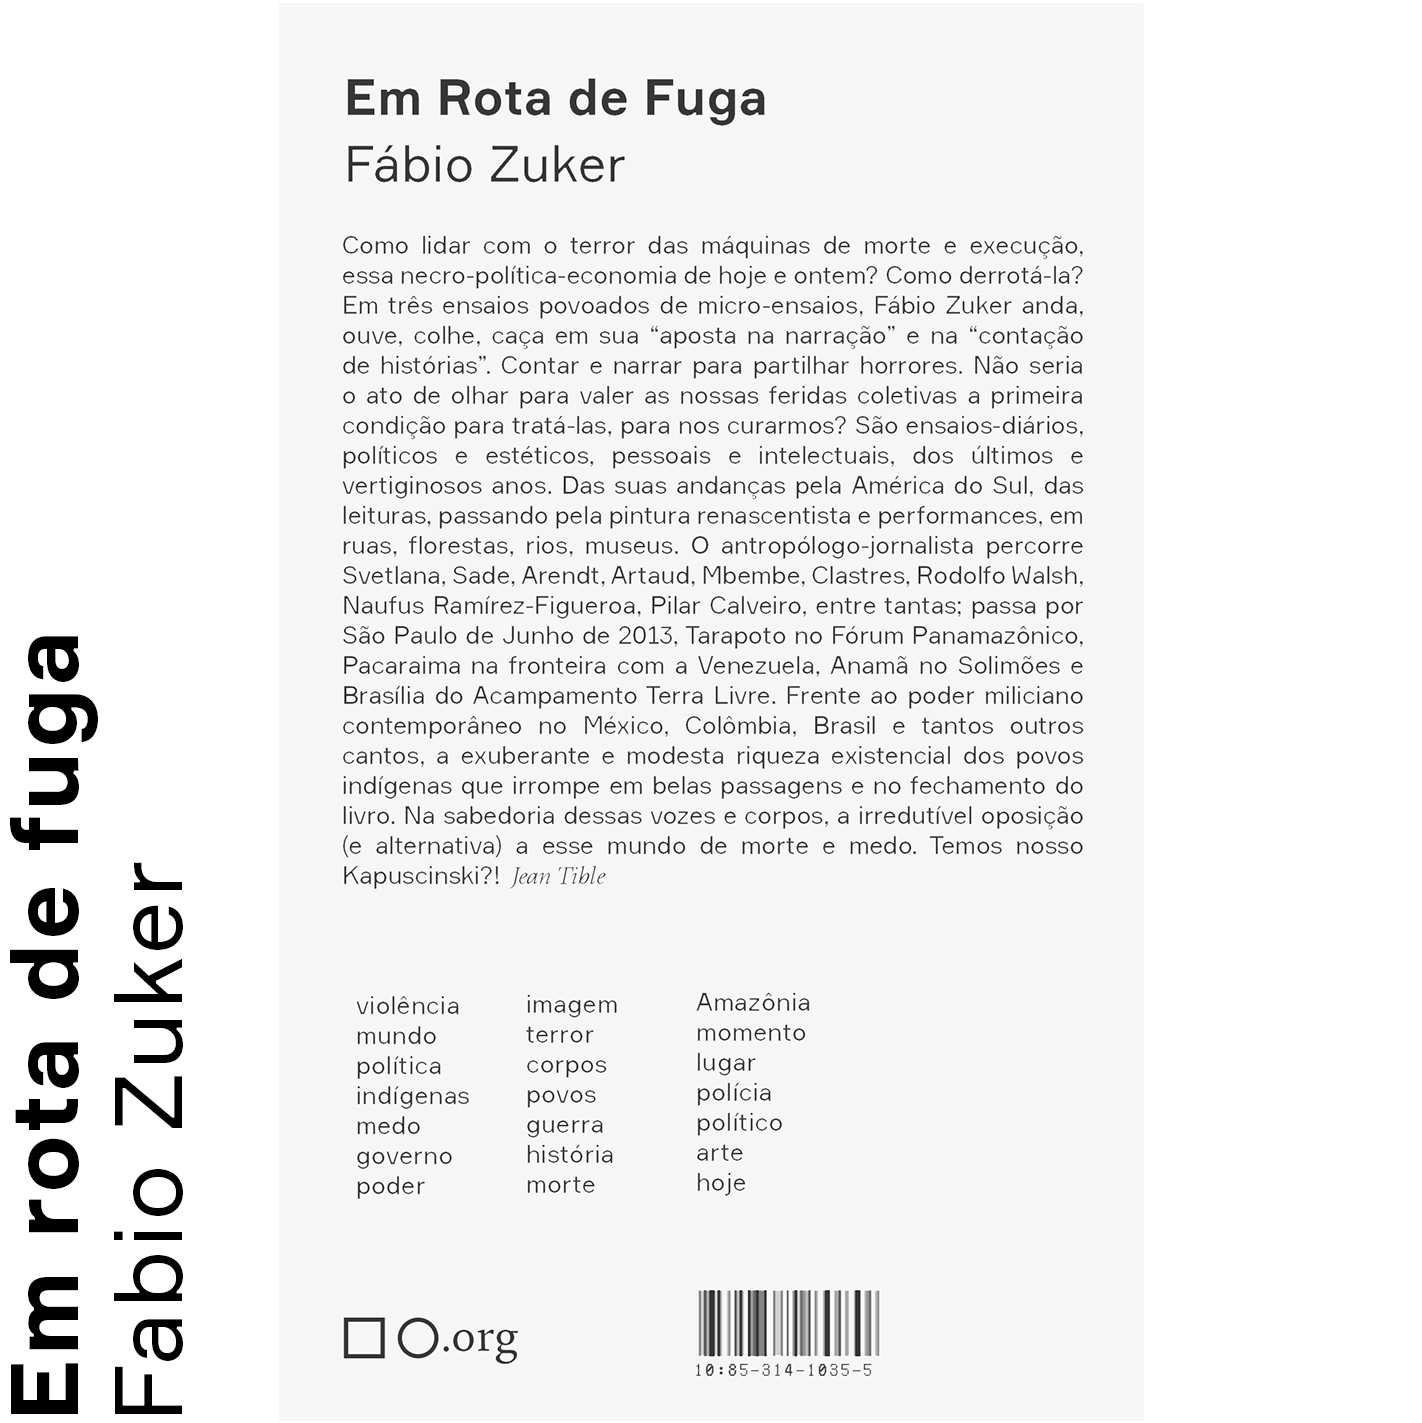
\includegraphics[width=40mm]{./grid2/zuker.jpg}}
\subfloat{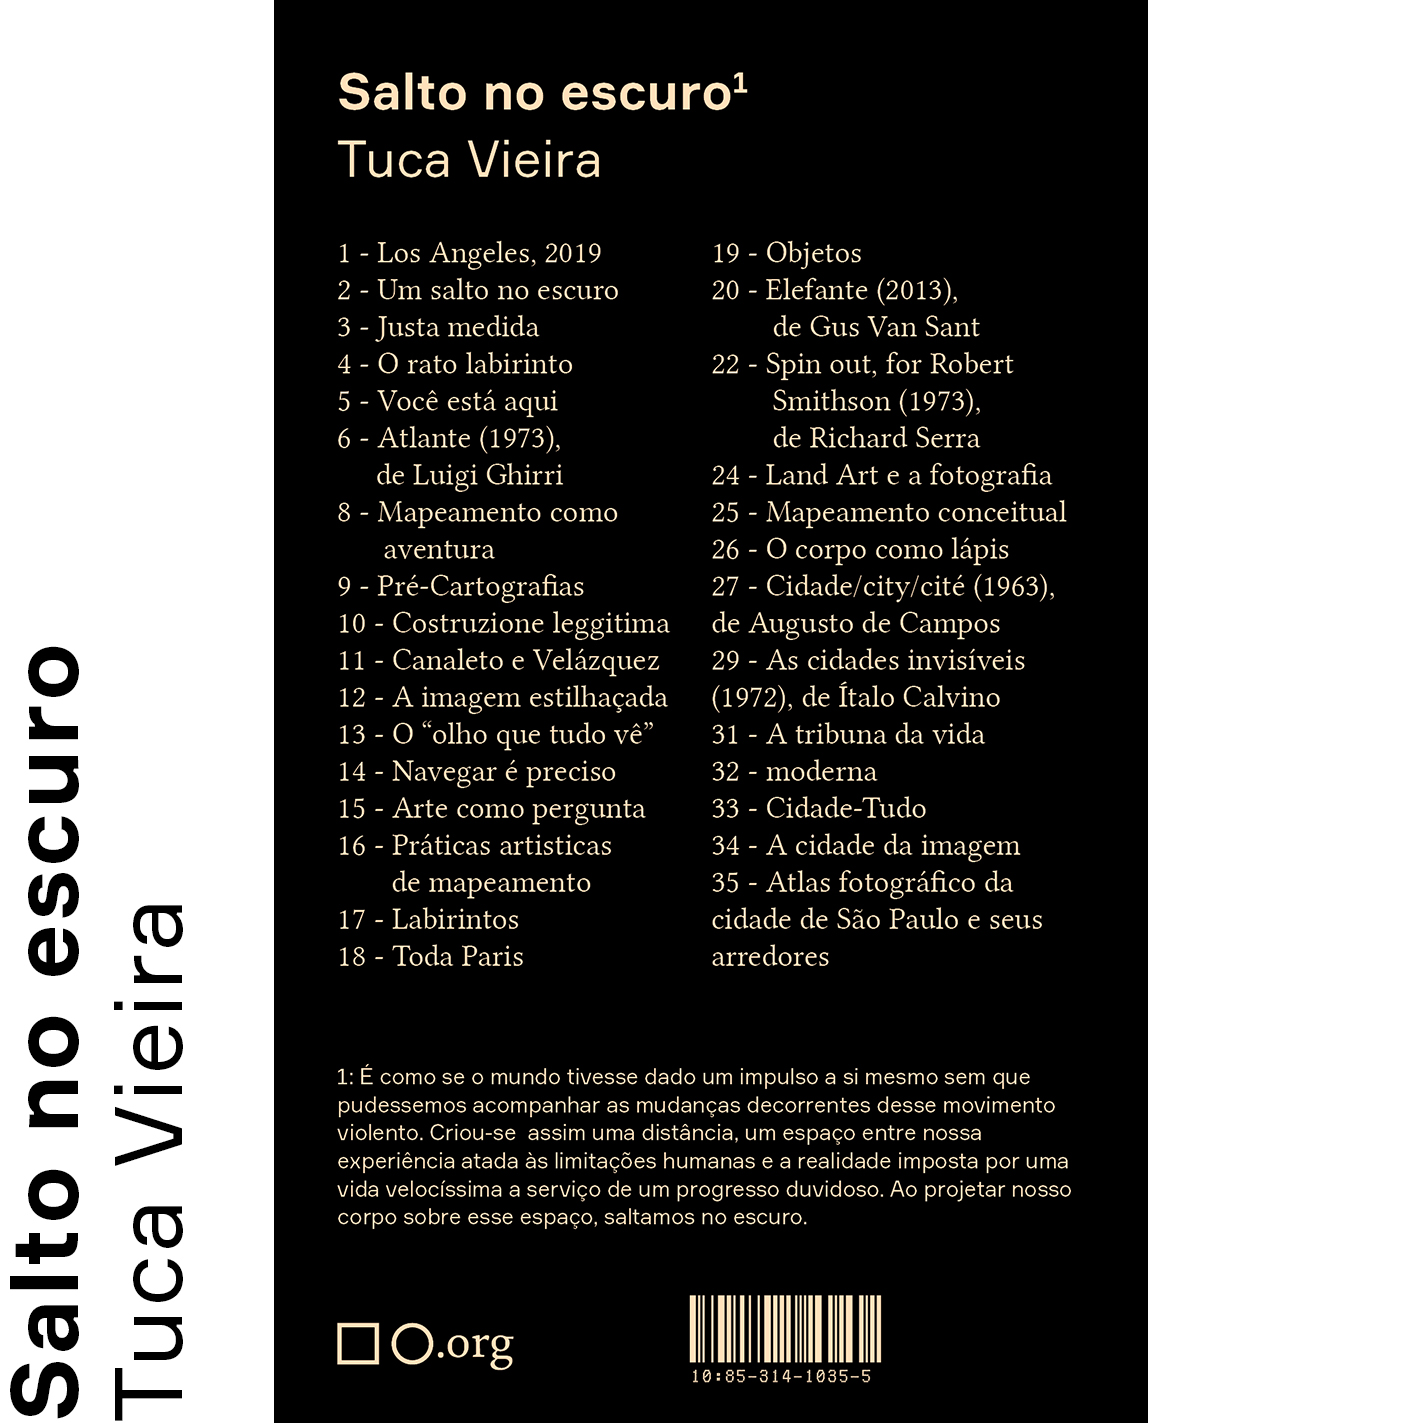
\includegraphics[width=40mm]{./grid2/tuca.jpg}}\\
\end{tabular}
\end{figure}

\pagebreak

%\vspace*{.1cm}
%
%\begin{figure}[!htbp]
%\begin{tabular}{cccc}
%
%\vspace{.5cm}
%\hspace*{-.5cm}
%\subfloat{\includegraphics[width=41mm]{./grid/tembeta.jpg}}\\\hspace*{-.5cm}
%\subfloat{\includegraphics[width=41mm]{./grid/mautner.jpg}}
%\subfloat{\includegraphics[width=41mm]{./grid/lage.jpg}}
%\subfloat{\includegraphics[width=41mm]{./grid/hotel.jpg}}
%
%\end{tabular}
%\end{figure}
%
%\pagebreak

\pagestyle{ayllon}
\label{ayllon}


\begin{textblock*}{5.625in}(0pt,0pt)%
\vspace*{-1.45cm}
\hspace*{-1.2cm}\includegraphics*[width=112mm]{./imgs/AYLLON.png}
\end{textblock*}

\pagebreak

\hspace{.5cm}

\begin{center}
\hspace*{-.5cm}\includegraphics[width=50mm]{./imgs/cabalat.png}
\end{center}

\hspace*{-7cm}\hrulefill\hspace*{-7cm}

\medskip

\noindent{}{\slsc{Cabalat shabat: poemas rituais}} reúne cinco textos, tratados aqui como poemas --- rezas e bênçãos judaicas --- e entoados na cerimônia de cabalat shabat, o recebimento do shabat a partir do pôr"-do"-sol da sexta"-feira. De teor místico, as canções são aqui apresentadas de maneira secular mas não anti"-religiosa. Em tradução do hebraico, sua temática situa"-se em paralelo a outros lugares poéticos da Antiguidade, trazendo no próprio ritual um entendimento estrutural e histórico do judaísmo. %493

%\hspace{.5cm}
\vfill

%\begin{wraptable}{l}{15cm}
\hspace*{-.4cm}\begin{minipage}[c]{1\linewidth}
\small{
{\Formular{\textbf{
\hspace*{-.1cm}Título: Cabalat Shabat\\
Autor: Fabiana Grinberg (.org)\\ 
Editora: Ayllon\\
Páginas: 28\\
Formato: 17,1x26,7cm\\
Preço: R\$ 29,90\\
ISBN: 978-85-7715-610-8
}}}}
\end{minipage}
%\end{wraptable}


\pagebreak

\hspace{.5cm}

\begin{center}
\hspace*{-2.8cm}\raisebox{5.5cm}{\rotatebox[origin=t]{90}{\Formular{\textbf{Lançamento}}}}
\hspace*{2cm}\includegraphics[width=42mm]{./imgs/sebastian.png}
\end{center}

\hspace*{-7cm}\hrulefill\hspace*{-7cm}

\medskip

\noindent{}A narrativa de {\slsc{Fragmentos de um diário encontrado}} é constituída em torno da figura de alguém que se entrega aos labirintos urbanos parisienses em busca de algo tão perdido quanto indefinível: através das passagens desse diário o autor anônimo encarna o olhar do errante sobre a cidade. De 1932, a obra está afinada com o caráter rebelde das vanguardas artísticas europeias das décadas de 20 e 30, que influenciaram o autor e outros literatos romenos de seu tempo (Cioran, Ionesco, Eliade).

%\hspace{.5cm}
\vfill

\hspace*{-.4cm}\begin{minipage}[c]{1\linewidth}
\small{
{\Formular{\textbf{
\hspace*{-.1cm}Título: Fragmentos de um diário encontrado\\
Autor: Mihail Sebastián\\ 
Editora: Ayllon\\
Páginas: 55\\
Formato: 11x18cm\\
Preço: R\$ 29,90\\
ISBN: 978-85-7715-620-7
}}}}
\end{minipage}

\pagebreak

\pagestyle{azougue}
\label{azougue}

\hspace{.5cm}

\begin{center}
\hspace*{-1cm}\raisebox{5.5cm}{\rotatebox[origin=t]{90}{\Formular{\textbf{Lançamento}}}}
\hspace{1cm}\includegraphics[width=70mm]{eco.jpeg}
\end{center}

\hspace*{-2cm}\_\_\_\_\_\_\_\_\_\_\_\_\_\_\_\_\_\_\_\_\_\_\_\_\_\_\_\_\_\_\_\_\_\_\_\_\_\_\_\_\_\_\_\_\_\_\_\_\_\_\_\_\_\_\_\_\_\_\_\_\_\_\_\_\_\_\_\_\_\_\_\_\_\_

\noindent{}Lorem ipsum dolor sit amet, consectetur adipiscing elit.
Donec sodales tortor a purus accumsan, ut ultricies purus
maximus. Aliquam bibendum consequat mi, sed commo-
do velit pellentesque id. Vivamus ultricies ligula in semper
sagittis. Donec mollis odio in lectus tristique, sed convallis
est interdum. Cras eget sem condimentum, pretium purus
eu, auctor.

\hspace{.5cm}

\hspace*{-.4cm}\begin{minipage}[c]{0.45\linewidth}
\small{
{\Formular{\textbf{
\hspace*{-.1cm}Título: Ecopolítica\\
Autor: Edson Passetti\\ 
Editora: Hedra\\
Páginas: 476\\
Formato: 23x16cm\\
Preço: R\$ 79,90\\
}}}}
\end{minipage}
\begin{minipage}[c]{0.50\linewidth}
\small{Lorem ipsum dolor sit amet, consectetur adipiscing elit.
Donec sodales tortor a purus accumsan, ut ultricies. Lorem ipsum dolor sit amet, consectetur adipiscing elit. Lorem ipsum dolor sit amet. Lorem ipsum dolor sit amet.} 
\end{minipage}

\pagebreak

\hspace{.5cm}

\begin{center}
\hspace*{-.5cm}\includegraphics[width=70mm]{eco.jpeg}
%\hspace*{6cm}\raisebox{2cm}{\rotatebox[origin=t]{90}{\Formular{\textbf{Lançamento}}}}
\end{center}

\hspace*{-2cm}\_\_\_\_\_\_\_\_\_\_\_\_\_\_\_\_\_\_\_\_\_\_\_\_\_\_\_\_\_\_\_\_\_\_\_\_\_\_\_\_\_\_\_\_\_\_\_\_\_\_\_\_\_\_\_\_\_\_\_\_\_\_\_\_\_\_\_\_\_\_\_\_\_\_

\noindent{}Lorem ipsum dolor sit amet, consectetur adipiscing elit.
Donec sodales tortor a purus accumsan, ut ultricies purus
maximus. Aliquam bibendum consequat mi, sed commo-
do velit pellentesque id. Vivamus ultricies ligula in semper
sagittis. Donec mollis odio in lectus tristique, sed convallis
est interdum. Cras eget sem condimentum, pretium purus
eu, auctor.

\hspace{.5cm}

\hspace*{-.4cm}\begin{minipage}[c]{0.45\linewidth}
\small{
{\Formular{\textbf{
\hspace*{-.1cm}Título: Ecopolítica\\
Autor: Edson Passetti\\ 
Editora: Hedra\\
Páginas: 476\\
Formato: 23x16cm\\
Preço: R\$ 79,90\\
}}}}
\end{minipage}
\begin{minipage}[c]{0.50\linewidth}
\small{Lorem ipsum dolor sit amet, consectetur adipiscing elit.
Donec sodales tortor a purus accumsan, ut ultricies. Lorem ipsum dolor sit amet, consectetur adipiscing elit. Lorem ipsum dolor sit amet. Lorem ipsum dolor sit amet.} 
\end{minipage}

\pagebreak

\hspace{.5cm}

\begin{center}
\hspace*{-1cm}\raisebox{5.5cm}{\rotatebox[origin=t]{90}{\Formular{\textbf{Lançamento}}}}
\hspace{1cm}\includegraphics[width=70mm]{eco.jpeg}
\end{center}

\hspace*{-2cm}\_\_\_\_\_\_\_\_\_\_\_\_\_\_\_\_\_\_\_\_\_\_\_\_\_\_\_\_\_\_\_\_\_\_\_\_\_\_\_\_\_\_\_\_\_\_\_\_\_\_\_\_\_\_\_\_\_\_\_\_\_\_\_\_\_\_\_\_\_\_\_\_\_\_

\noindent{}Lorem ipsum dolor sit amet, consectetur adipiscing elit.
Donec sodales tortor a purus accumsan, ut ultricies purus
maximus. Aliquam bibendum consequat mi, sed commo-
do velit pellentesque id. Vivamus ultricies ligula in semper
sagittis. Donec mollis odio in lectus tristique, sed convallis
est interdum. Cras eget sem condimentum, pretium purus
eu, auctor.

\hspace{.5cm}

\hspace*{-.4cm}\begin{minipage}[c]{0.45\linewidth}
\small{
{\Formular{\textbf{
\hspace*{-.1cm}Título: Ecopolítica\\
Autor: Edson Passetti\\ 
Editora: Hedra\\
Páginas: 476\\
Formato: 23x16cm\\
Preço: R\$ 79,90\\
}}}}
\end{minipage}
\begin{minipage}[c]{0.50\linewidth}
\small{Lorem ipsum dolor sit amet, consectetur adipiscing elit.
Donec sodales tortor a purus accumsan, ut ultricies. Lorem ipsum dolor sit amet, consectetur adipiscing elit. Lorem ipsum dolor sit amet. Lorem ipsum dolor sit amet.} 
\end{minipage}

\pagebreak

\hspace{.5cm}

\begin{center}
\hspace*{-.5cm}\includegraphics[width=70mm]{eco.jpeg}
%\hspace*{6cm}\raisebox{2cm}{\rotatebox[origin=t]{90}{\Formular{\textbf{Lançamento}}}}
\end{center}

\hspace*{-2cm}\_\_\_\_\_\_\_\_\_\_\_\_\_\_\_\_\_\_\_\_\_\_\_\_\_\_\_\_\_\_\_\_\_\_\_\_\_\_\_\_\_\_\_\_\_\_\_\_\_\_\_\_\_\_\_\_\_\_\_\_\_\_\_\_\_\_\_\_\_\_\_\_\_\_

\noindent{}Lorem ipsum dolor sit amet, consectetur adipiscing elit.
Donec sodales tortor a purus accumsan, ut ultricies purus
maximus. Aliquam bibendum consequat mi, sed commo-
do velit pellentesque id. Vivamus ultricies ligula in semper
sagittis. Donec mollis odio in lectus tristique, sed convallis
est interdum. Cras eget sem condimentum, pretium purus
eu, auctor.

\hspace{.5cm}

\hspace*{-.4cm}\begin{minipage}[c]{0.45\linewidth}
\small{
{\Formular{\textbf{
\hspace*{-.1cm}Título: Ecopolítica\\
Autor: Edson Passetti\\ 
Editora: Hedra\\
Páginas: 476\\
Formato: 23x16cm\\
Preço: R\$ 79,90\\
}}}}
\end{minipage}
\begin{minipage}[c]{0.50\linewidth}
\small{Lorem ipsum dolor sit amet, consectetur adipiscing elit.
Donec sodales tortor a purus accumsan, ut ultricies. Lorem ipsum dolor sit amet, consectetur adipiscing elit. Lorem ipsum dolor sit amet. Lorem ipsum dolor sit amet.} 
\end{minipage}

\pagebreak
\pagestyle{circuito}
\label{circuito}

\begin{textblock*}{5.625in}(0pt,0pt)%
\vspace*{-3.5cm}
\hspace*{-2.77cm}\includegraphics*[width=175.2mm]{./propagandas/CIRCUITO.pdf}
\end{textblock*}

\pagebreak %AS ARTES DO COVER


\begin{center}
\hspace*{-3.6cm}\raisebox{5cm}{\rotatebox[origin=t]{90}{\huge\Formular{\textbf{Lançamento}}}}
\hspace*{3.1cm}\includegraphics[width=74mm]{./grid/cover.jpg}
\end{center}

\hspace*{-7cm}\hrulefill\hspace*{-7cm}

\medskip

\noindent{}Noção de origem, original, único, essência originária. O que é afirmado ao dizermos que algo é original? Desde Aristóteles já se sabe que a imitação – ou mímesis – deveria recriar a potência de vida e não sua forma. É com base nesse pensamento que o autor pode afirmar que o cover é também uma criação, mesmo relacionado à sua base precedente e sem qualquer hierarquia preestabelecida. O cover inventa outro original.
A origem passa então a ser um início que se recria em {\slsc{continuum}}, sempre presentificada em ato, um simulacro com força de raiz: a presente obra repensa a noção de presente e de presença através do cover. Uma presença pensada como acontecimento subversivo, que borra as linhas que separam o “mesmo” do “diferente”, o “original” do “simulacro”, e concretiza passado e presente no mesmo ato. O cover como pulso da repetição do dessemelhante, como inventividade plena. Quem veio primeiro, o ovo ou a galinha? A leitura de {\slsc{As artes do cover}}, escrito pelo diretor de teatro, performer, professor, curador e crítico Henrique Saidel, nos permite vê"-los juntos em ato, no mesmo tempo"-espaço de criação.

\vfill

\hspace*{-.4cm}\begin{minipage}[c]{.5\linewidth}
\small{
{\Formular{\textbf{
\hspace*{-.1cm}\hlc[lightyellow]{Editora: Circuito}\\
Título: As artes do cover\\
Autor: Henrique Saidel\\ 
ISBN: 978-85-9582-049-4\\
Páginas: 352\\
Formato: 14x21cm\\
Preço: R\$ 55,00\\
Disponibilidade: Disponível
}}}}
\end{minipage}

\pagebreak %TODOS OS LUGARES


\begin{center}
\hspace*{.5cm}\includegraphics[width=74mm]{./grid/lugares.jpg}
\end{center}

\hspace*{-7cm}\hrulefill\hspace*{-7cm}

\medskip

\noindent{}{\slsc{Todos os lugares}} trata"-se de um glossário, escrito e ilustrado pelas talentosas mãos de Alex Ceverny, artista plástico, desenhista, gravador, escultor, ilustrador e pintor. Percorre cidades e lugares onde esteve, tecendo comentários “de uma observação ferina e fértil, aguda sensibilidade e humor irônico quase mordaz”, engendrando assim “espaços e situações singulares, quase oníricos e belos; mundos solitários com os quais de algum modo sonhamos e de alguma forma aspiramos habitar”, conforme escreve Renato Rezende no prefácio.

Um dos mais notáveis artistas brasileiros da atual geração, Ceverny produz em suas viagens peregrinações e inflexões sobre si próprio, dividindo uma vida rica e cuidadosamente enlaçada entre imagem e escrita, entre “riscos, traços e viagens”. Belo e singular, o livro conta também com prefácio do curador Renato Rezende e posfácio do escritor e filósofo Rodrigo Petronio.

\vfill

\hspace*{-.4cm}\begin{minipage}[c]{.5\linewidth}
\small{
{\Formular{\textbf{
\hspace*{-.1cm}\hlc[lightyellow]{Editora: Circuito}\\
Título: Todos os lugares\\
Autor: Alex Cerveny\\ 
ISBN: 978-85-9582-050-0\\
Páginas: 190\\
Formato: 16x23cm\\
Preço: R\$ 80,00\\
Disponibilidade: Disponível
}}}}
\end{minipage}

\pagebreak

\vspace*{1.5cm}

\noindent{}{\nohyphens{\LARGE{Entre todos os lugares\\\noindent{}{\large\slsc{Riscos, traços, viagens: é pelo desenho que o pensamento encarnado\\ em uma pintura se dá a perceber, que o pensamento se une ao sensível}}}}}

\bigskip

\hfill{}\scalebox{.8}{RENATO REZENDE}

\bigskip
\bigskip
\bigskip


Sobretudo um poeta, o pintor e gravurista Alex Cerveny é dotado de imaginação ferina e fértil, aguda sensibilidade e humor irônico e quase mordaz. Espaços e situações singulares, quase"-oníricos e belos, mundos solitários com os quais de algum modo sonhamos e de alguma forma aspiramos habitar: há algo na estranheza das imagens do artista com que nos identificamos atavicamente, e suas superfícies planas — raramente faz uso de perspectiva, mas adota efeitos de sombra e luz, criando volumes ilusórios — funcionam como uma espécie de espelho de algum nosso mundo interior silencioso (mas sempre à beira de dizer algo) e perdido, possivelmente na infância.

Fundamentalmente lírico e fabular em seu afã elaborador, como um criador de mitos — não seria este fundamentalmente o lugar do artista? —, compreendendo perfeitamente e comentando com astúcia e certa compaixão a complexidade e sublimidade do mundo contemporâneo, é capaz de transubstanciá"-lo em narrativas plenas de espiritualidade, sentido e humanidade.

O êxito de sua complexa linguagem poética é também fruto da salutar distância que Alex Cerveny sempre soube manter, escolhendo o caminho de uma trajetória praticamente autodidata, dos imperativos do mercado, e de sua autonomia em relação aos movimentos geracionais. Muito embora possamos situá"-lo historicamente como integrante da fecunda geração 1980, que se revela muito mais rica do que a produção de pintura expressiva e gestual que logo de cara alcançou reconhecimento. 

É também reconhecido e premiado ilustrador (entre outros exemplos, seu exuberante trabalho para recentes edições de {\slsc{Pinóquio}}, {\slsc{Decameron}} e {\slsc{A origem das espécies}}, de Darwin), e eu não hesitaria em afirmá"-lo um mestre contemporâneo da iluminura. Não nos surpreende que em Alex Cerveny o livro, objeto próximo do mágico e do sagrado, ocupe um lugar seminal em seu universo artístico. 

Ao completar cinquenta anos, Alex Cerveny se deu de presente uma viagem à China — que resultou numa belíssima série de desenhos a nanquim sobre papel de arroz, alguns deles reproduzidos neste livro, e primeiramente exibidos na exposição {\slsc{Glossário dos nomes próprios}}, no Paço Imperial do Rio de Janeiro e na galeria Triângulo, em São Paulo, 2015. Não foi uma viagem qualquer: mas uma peregrinação de reflexão e ajuste de contas consigo mesmo. Neste momento mais maduro, Alex Cerveny estabelece cada vez mais seu lugar na arte contemporânea brasileira para muito além das demandas do mercado, com exposições como a individual {\slsc{Palimpsesto}} (Museu Lasar Segall), e a participação na mostra {\slsc{Nous les arbres}} (Fundação Cartier), em Paris, atraindo olhar da crítica e tornando"-se referência para novos artistas. 

Entre outros exemplos, Alex Cerveny é autor de um surpreendente livro"-objeto, em camadas"-gavetas e em forma de pirâmide, O desenho visto do céu, inspirado por suas viagens a Nazca, no Peru. {\slsc{Todos os lugares}} se apresenta como uma extensão ou inversão do seu trabalho como ilustrador, em que os textos são escritos para preencher espaços em branco, encaixados ali por se expressarem em letras, memórias que o artista gostaria de desenhar em detalhes: raro e feliz encontro da palavra e do traço do artista/poeta. O livro é um glossário de locais, cidades, vilarejos, montes ou lagoas, todos os lugares, ou quase todos, que esse artista andarilho visitou durante sua vida, encontrando pessoas, animais e objetos, coletando e oferecendo histórias, experiências e cuidados. 

Com o presente livro, divide cada detalhe de uma vida rica e cuidadosamente elaborada, assim como é elaborada sua obra. E uma completa cronologia do artista encontra"-se no final da publicação. {\slsc{Todos os lugares}} é uma compilação de poemas"-relatos, ou um tipo peculiar de livro de memórias, acompanhado por imagens, organizado pelo afeto, guiado pela beleza e impregnado de humor. "O que fazer com um pinguim perdido na neblina em estado de choque?", ele se pergunta, por exemplo, na praia da Jureia, em seu estado de São Paulo natal. Como responder? {\slsc{Todos os lugares}}, de Alex Cerveny, enlaça escrita e imagem pela costura lírica de suas vivências. Riscos, traços, viagens: é pelo desenho que o pensamento encarnado em uma pintura se dá a perceber, que o pensamento se une ao sensível. 

Particularmente, sinto"-me feliz e honrado por acompanhar a produção dessa obra única desde praticamente seus primeiros traços e passos. E por poder contribuir de alguma forma com este livro; por ter um lugar entre todos os lugares.\footnote{Adaptado do prefácio do livro {\slsc{Em todos os lugares}}.}

\pagebreak %ANTIFA

\begin{center}
\hspace*{-3.6cm}\raisebox{5cm}{\rotatebox[origin=t]{90}{\huge\Formular{\textbf{Lançamento}}}}
\hspace*{3.1cm}\includegraphics[width=74mm]{./grid/antifa.png}
\end{center}

\hspace*{-7cm}\hrulefill\hspace*{-7cm}

\medskip

\noindent{}A ascensão ao poder de uma direita radicalizada, nova sobretudo nos métodos de ação e no uso eficiente das tecnologias modernas, impõe uma reflexão de ordem tática: o que é, hoje, o antifascismo? Como a convulsão social pode organizar"-se contra o controle imposto por polícias ultraviolentas?
Se por um lado governantes como Jair Bolsonaro ou Donald Trump dispõem de amplo arsenal fático e bélico, a explosão recente de protestos pelo mundo aponta para uma janela de ação, em que a revolta popular também se radicaliza e, literalmente, coloca nações inteiras em chamas.

E é na esteira desse momento fundamental que é estruturado {\slsc{Antifa: modo de usar}}. A publicação reúne ensaios, textos e entrevistas do historiador americano Mark Bray, especialista no movimento antifascista e uma das principais vozes do momento de luta. Além de textos de Acácio Augusto --- organizador do volume, cientista social e pesquisador em estudos libertários do grupo Nu-Sol --- compondo um material urgente e essencial para nosso tempo.

\vfill

\hspace*{-.4cm}\begin{minipage}[c]{.5\linewidth}
\small{
{\Formular{\textbf{
\hspace*{-.1cm}\hlc[lightyellow]{Editora: Circuito \& Hedra}\\
Título: Antifa: modo de usar\\
Autor: Acácio Augusto (org.)\\ 
ISBN: 978-85-7715-652-8\\
Páginas: ???\\
Formato: 12,7x19,1cm\\
Preço: R\$ ????\\
Disponibilidade: 17/07/2020
}}}}
\end{minipage}

\pagebreak %INTRODUÇÃO À SOMA

\begin{center}
\hspace*{.5cm}\includegraphics[width=74mm]{./grid/soma.png}
\end{center}

\hspace*{-7cm}\hrulefill\hspace*{-7cm}

\medskip

\noindent{}{\slsc{Introdução à Soma: terapia e pedagogia anarquista do corpo}} trata de um processo terapêutico corporal realizado em grupo, que busca no pensamento anarquista uma crítica às mais variadas formas de poder impregnadas no comportamento individual e nas relações sociais. O grupo de terapia funciona como um micro"-laboratório social, no qual se desenvolve uma análise libertária do comportamento de cada um a partir da relação junto ao outro.

Daí sua originalidade: terapia como criação e afirmação de si, em que a construção das práticas de liberdade é o antídoto para combater os conflitos gerados pelas relações sociais hierarquizadas. A somaterapia ou apenas Soma é um processo terapêutico"-pedagógico, realizado em grupo e com ênfase na articulação entre o trabalho corporal e o uso da linguagem verbal. Foi criada no Brasil pelo escritor e terapeuta Roberto Freire, a partir da obra de Wilhelm Reich e sua pesquisa sobre corpo e emoção.

\vfill

\hspace*{-.4cm}\begin{minipage}[c]{.5\linewidth}
\small{
{\Formular{\textbf{
\hspace*{-.1cm}\hlc[lightyellow]{Editora: Circuito \& Hedra}\\
Título: Introdução à Soma — terapia\\ e pedagogia anarquista do corpo\\
Autor: João da Mata\\ 
ISBN: 978-85-9582-055-5\\
Páginas: 106\\
Formato: 12,7x19,1cm\\
Preço: R\$ 42,90\\
Disponibilidade: 17/07/2020
}}}}
\end{minipage}

\pagebreak %FILOSOFIA BLACK BLOC

\begin{center}
\hspace*{-3.6cm}\raisebox{5cm}{\rotatebox[origin=t]{90}{\huge\Formular{\textbf{Lançamento}}}}
\hspace*{3.1cm}\includegraphics[width=74mm]{./grid/black.png}
\end{center}

\hspace*{-7cm}\hrulefill\hspace*{-7cm}

\medskip

\noindent{}Em junho de 2013, data da maior erupção social das últimas décadas, o movimento {\slsc{Black Bloc}} ganhou os holofotes como nova prática de luta e manifestação. Analistas à direita e à esquerda foram forçados a tentar compreender o movimento, normalmente municiando um repertório conceitual incompatível com os significados do {\slsc{Black Bloc}}, sem entendê"-lo em seus próprios termos.

Procurando suprir essa carência surge o {\slsc{Filosofia Black Bloc}}, que concebe e mobiliza um arcabouço teórico que permita abordar o movimento {\slsc{Black Bloc}} como fenômeno: produzir, no pensamento, uma filosofia {\slsc{Black Bloc}}. Não cessamos de ler Junho sob o ponto de vista de Brasília, dos palácios de governo, dos partidos recusados pelas multidões, da surpresa e da inércia dos poderes constituídos, da decadência da representação formal, das classes cerradas para o social. Pensar Junho nesses termos torna"-se então “capturar e destruir” sua potência específica. Não é por acaso que boa parte das interpretações de intelectuais se parece tanto com os discursos da grande imprensa que vimos circular.


\vfill

\hspace*{-.4cm}\begin{minipage}[c]{.5\linewidth}
\small{
{\Formular{\textbf{
\hspace*{-.1cm}\hlc[lightyellow]{Editora: Circuito \& Hedra}\\
Título: Filosofia Black Bloc\\
Autor: Murilo Duarte Costa Correa\\ 
ISBN: 978-85-9582-056-2\\
Páginas: 166\\
Formato: 12,7x19,1cm\\
Preço: R\$ 46,90\\
Disponibilidade: 17/07/2020
}}}}
\end{minipage}


\pagebreak %1967, MEIO SÉCULO DEPOIS


\begin{center}
\hspace*{.5cm}\includegraphics[width=74mm]{./grid/1967.png}
\end{center}

\hspace*{-7cm}\hrulefill\hspace*{-7cm}

\medskip

\noindent{}{\slsc{1967, meio século depois}} é um livro que sonda --- na confluência das artes plásticas, literatura, cinema, \scalebox{.8}{TV}, teatro e política --- o ano de 1967 e seus principais desdobramentos no pensamento e na cultura brasileira. Diversos ensaístas e intelectuais analisam no livro temas como o tropicalismo, os festivais de música, as revoluções perpetradas por Zé Celso no Teatro Oficina, o Cinema Novo de Glauber Rocha e as provocantes obras de Hélio Oiticica.

Às vésperas do período mais ditatorial e repressivo da história brasileira, as artes tentaram abrir  caminhos de liberdade e insurgência de um Brasil plurívoco e múltiplo, nos quais os autores procuram linhas de permanências e rupturas cinquenta anos depois. Como escreve Frederico Coelho, um dos organizadores do volume, fazer esse balanço serve de “alerta dentre as novas gerações cuja leitura pode cada vez mais se aproximar daquele momento dramático pela lente absurda de nosso presente”, em um tempo que a missão do intelectual é entender que “diagnósticos precários se tornaram parte de nosso cotidiano na luta contra a linha evolutiva do conservadorismo brasileiro”.


\vfill
\enlargethispage{\baselineskip}

\hspace*{-.4cm}\begin{minipage}[c]{1\linewidth}
\small{
{\Formular{\textbf{
\hspace*{-.1cm}\hlc[lightyellow]{Editora: Circuito \& Editora PUC-Rio}\\
Título: 1967, meio século depois\\
Autor: Felipe Scovino, Fred Coelho,\\ Pedro Duarte e Sérgio Martins (orgs.)\\ 
ISBN: 978-85-9582-057-9\\
Páginas: 268\\
Formato: 16x23cm\\
Preço: R\$ ????\\
Disponibilidade: 28/08/2020
}}}}
\end{minipage}

\pagebreak

\pagestyle{circuitocat}

\begin{multicols}{2}
\begin{enumerate}
\raggedright\nohyphens{
\item A grande marcha, {\Formular{\textbf{Ewerton Martins Ribeiro }}}
\item A loucura branca, {\Formular{\textbf{Jaime Rocha}}}
\item A outra morte de Alberto Caeiro, {\Formular{\textbf{Afonso Henriques Neto}}}
\item A Dialética do gosto, {\Formular{\textbf{Marco Scheinder}}}
\item Adoecer, {\Formular{\textbf{Hélia Correia}}}
\item Almas selvagens, {\Formular{\textbf{André Gardel}}}
\item Até ano que vem em Jerusalém, {\Formular{\textbf{Maria da Conceição Caleiro}}}
\item Cadernos de artista, {\Formular{\textbf{Moisés Alves}}}
\item Cérebro-Ocidente/Cérebro"-Brasil, {\Formular{\textbf{Roberto Corrêa dos Santos}}}
\item Nove tiros em Chef Lidu, {\Formular{\textbf{Paula Bajer Fernandes}}}
\item Comunidades sem fim
\item Coletivos
\item DJs
\item Dezembro, {\Formular{\textbf{Ana Tereza Salek}}}
\item Os tigres cravaram as garras no horizonte, {\Formular{\textbf{Augusto Guimaraens Cavalcanti}}}
\item No contemporâneo: arte e escritura expandidas, {\Formular{\textbf{Roberto Corrêa dos Santos; Renato Rezende}}}
\item Truques de autor, {\Formular{\textbf{Heleno Bernardi}}}
\item Clínica de artista I, {\Formular{\textbf{Roberto Corrêa dos Santos}}}
\item Clínica de artista II, {\Formular{\textbf{Roberto Corrêa dos Santos}}}
\item Vertigens, {\Formular{\textbf{Fernanda de Mello Gentil}}}
\item Nós somos uma correspondência, {\Formular{\textbf{Fernanda de Mello Gentil}}}
\item Amarração, {\Formular{\textbf{Renato Rezende}}}
\item Conversas com curadores e críticos de arte
\item Experiência e arte contemporânea
\item Romance, {\Formular{\textbf{Caio Meira}}}
\item Auréola, {\Formular{\textbf{Renato Rezende}}}
\item Cosmocrunch, {\Formular{\textbf{Maria Dolores Wanderley}}}
\item Preces para a amiga submersa, {\Formular{\textbf{Lucia Castello Branco}}}
\item Pequena coleção de grandes horrores, {\Formular{\textbf{Luiz Brás}}}
\item Nós, o outro, o distante na arte brasileira contemporânea, {\Formular{\textbf{Marisa Flórido Cesar}}}
\item Lira dos sentidos, {\Formular{\textbf{Carlos Henrique Costa}}}
\item Rasga-mortalha: poemas dos outros, {\Formular{\textbf{W. B. Lemos}}}
\item Os nomes, {\Formular{\textbf{Rogério Luz}}}
\item N’Ágorainda, {\Formular{\textbf{Naila Rachid}}}
\item O ser-se, {\Formular{\textbf{Júnia Azevedo}}}
\item A reflexão atuante, {\Formular{\textbf{Sergio Cohn}}}
\item Intervenções críticas, {\Formular{\textbf{Josefina Ludmer}}}
\item O homem mais portátil do mundo, {\Formular{\textbf{Arturo Carrera}}}
\item O capitão Nemo e eu, {\Formular{\textbf{Alfredo Prior}}}
\item Notas, disparos, sublinhados, {\Formular{\textbf{María Moreno}}}
\item Naxos, {\Formular{\textbf{Elsa Cross}}}
\item Diário em progresso, {\Formular{\textbf{Alex Frechette}}}
\item Em caso de emergência pare o tempo, {\Formular{\textbf{Gab Marcondes}}}
\item 1,68 x 1,81, {\Formular{\textbf{Maria André Leite}}}
\item Do tudo e do todo, {\Formular{\textbf{Cláudio Oliveira}}}
\item S.O.S. Poesia, {\Formular{\textbf{Renato Rezende; Dirk Vollenbroich}}}
\item O olho do lince, {\Formular{\textbf{Guilherme Zarvos}}}
\item Diário para descolorir, {\Formular{\textbf{Alex Frechette}}}
\item A pequena voz do mundo, {\Formular{\textbf{Diana Bellessi}}}
\item Amazônia \& Co., {\Formular{\textbf{Rafael Cippolini}}}
\item Fala, poesia, {\Formular{\textbf{Tamara Kamenszain}}}
\item Suturas. Um breviário, {\Formular{\textbf{Daniel Link}}}
\item Repetir, {\Formular{\textbf{Katia Maciel}}}
\item Coreografia (Orelhas contemporâneas), {\Formular{\textbf{André Parente}}}
\item Amor: verso: reverso (Orelhas contemporâneas), {\Formular{\textbf{Luiz Sérgio de }}}Oliveira
\item Saudades de um punhal (Orelhas contemporâneas), {\Formular{\textbf{Leila Danziger}}}
\item Gravidade (Orelhas contemporâneas), {\Formular{\textbf{Katia Maciel}}}
\item Artexperiência contemporânea (Orelhas contemporâneas), {\Formular{\textbf{Renato }}}Rezende
\item Práticas contemporâneas do mover-se, {\Formular{\textbf{Michelle Sommer}}}
\item Levantem lentamente o lençol, {\Formular{\textbf{Bia Albernaz}}}
\item Escritos sobre fotografia contemporânea brasileira
\item Doctypes, {\Formular{\textbf{Alex Hamburger}}}
\item Quarenta e quatro, {\Formular{\textbf{Mauricio Cardozo}}}
\item Ninfas e Mariposas, {\Formular{\textbf{Leonardo Toledo}}}
\item Lab Criativo / Creative Lab
\item Quase-poesia, {\Formular{\textbf{Jerson Lima Silva}}}
\item Música Chama, {\Formular{\textbf{Pedro Sá Moraes; Eduardo Guerreiro B. Losso}}}
\item Viventes de Saturno, {\Formular{\textbf{Carlos Frederico Manes}}}
\item Esperando a hora da Stella, {\Formular{\textbf{Maria Dolores Wanderley}}}
\item Falar o que seja é inútil – ou sobre desconsiderações, {\Formular{\textbf{Carlos Alberto Gianotti}}}
\item Lótus molotov, {\Formular{\textbf{Leonardo Toledo}}}
\item Outras margens, {\Formular{\textbf{Sergio Cohn}}}
\item Formas híbridas, {\Formular{\textbf{Rafael Gutiérrez}}}
\item Fornicar e matar e outros ensaios, {\Formular{\textbf{Laura Klein}}}
\item Cores cobras pincéis cães, {\Formular{\textbf{Eduardo Stupía}}}
\item Lasca de breu, {\Formular{\textbf{Guilherme Delgado}}}
\item O tropo tropicalista, {\Formular{\textbf{João Camillo Penna}}}
\item Leituras furadas, {\Formular{\textbf{Luis Felipe Fabre}}}
\item Escrever sobre escrever poesia, {\Formular{\textbf{Eduardo Milán}}}
\item A liberação da mosca, {\Formular{\textbf{Luigi Amara}}}
\item Mudança, {\Formular{\textbf{Verónica Gerber Bicecci}}}
\item Onde late um cachorro doido, {\Formular{\textbf{Moisés Alves}}}
\item Daniel Acosta
\item Éter, {\Formular{\textbf{António Cabrita}}}
\item Noturno Europeu, {\Formular{\textbf{Rui Nunes}}}
\item Café irlandês, {\Formular{\textbf{Barbosa Lagos}}}
\item Voo, {\Formular{\textbf{Ana Paula Simonaci}}}
\item Fim do Infante, {\Formular{\textbf{Marina Marcondes Machado}}}
\item 2013, memórias e resistências, {\Formular{\textbf{Camila Jourdan}}}
\item Escrito e dirigido por Moisés Alves, {\Formular{\textbf{Moisés Alves}}}
\item Coisas que fiz e ninguém notou mas que mudaram tudo, {\Formular{\textbf{Moisés Alves}}}
\item A cena lenta, {\Formular{\textbf{Cláudio Oliveira}}}
\item Copa pra quem? Olimpíadas pra quem?, {\Formular{\textbf{Alex Frechette}}}
\item O fantasma de um nome (poesia, imaginário, vida), {\Formular{\textbf{Jorge Monteleone}}}
\item Peso Morto, {\Formular{\textbf{João Felipe Gremski}}}
\item Romance de asilo, {\Formular{\textbf{André Monteiro}}}
\item Quem apaga a luz sou eu, {\Formular{\textbf{Magda Romano}}}
\item As artes do cover, {\Formular{\textbf{Henrique Saidel}}}
\item Frestas, {\Formular{\textbf{André Gardel}}}
\item O antes é o depois, {\Formular{\textbf{Guidi Vieira}}}
\item Humano, {\Formular{\textbf{Pedro Poeta}}}
}
\end{enumerate}
\end{multicols}

\pagebreak

\pagestyle{hedra}
\label{hedra}

\begin{textblock*}{5.625in}(0pt,0pt)%
\vspace*{-3.5cm}
\hspace*{-2.77cm}\includegraphics*[width=175.2mm]{./propagandas/HEDRA.pdf}
\end{textblock*}

\pagebreak


\begin{center}
\hspace*{-3.6cm}\raisebox{5cm}{\rotatebox[origin=t]{90}{\huge\Formular{\textbf{Lançamento}}}}
\hspace*{3.1cm}\includegraphics[width=74mm]{./grid/passetti.jpeg}
\end{center}

\hspace*{-7cm}\hrulefill\hspace*{-7cm}

\medskip

\noindent{}Na ecopolítica o alvo principal dos governos é o planeta, visando recuperar sua vida degradada e conservá"-lo de modo sustentável, em benefício das futuras gerações. Pressiona os regimes políticos para a democracia em sintonia com a racionalidade neoliberal. Pretende dar conta não só do governo da espécie humana, mas dos viventes na Terra.

Fruto de reuniões de estudiosos anarquistas, \hlc[lightyellow]{``Ecopolítica'' mapeia a passagem da biopolítica --- o controle da vida analisado por Foucault 	--- para a ecopolítica}, nova forma de governar que emerge pós"-\scalebox{.8}{II} Guerra Mundial e com as institucionalizações subsequentes, e se estende a todas as esferas do mundo natural. O grupo libertário Nu"-Sol percorre e analisa acontecimentos históricos e contemporâneos, e atravessa fluxos de poder para conclamar à criação de resistências libertárias e esquivas às globalizantes linhas de controle.

\vfill

\hspace*{-.4cm}\begin{minipage}[c]{.5\linewidth}
\small{
{\Formular{\textbf{
\hspace*{-.1cm}\hlc[lightyellow]{Editora: Hedra}\\
Título: Ecopolítica\\
Autor: Edson Passetti (org.)\\ 
ISBN: 978-85-7715-609-2\\
Páginas: 476\\
Formato: 16x23cm\\
Preço: R\$ 79,90\\
Disponibilidade: Disponível
}}}}
\end{minipage}


\pagebreak


\begin{center}
\hspace*{.5cm}\includegraphics[width=74mm]{./grid/freud.png}
\end{center}

\hspace*{-7cm}\hrulefill\hspace*{-7cm}

\medskip

\noindent{}{\slsc{Freud e o patriarcado}} parte da constatação de que a teoria psicanalítica põe em jogo uma forma de conceber o psíquico --- ou a subjetividade --- como algo construído a partir de um modelo que assume uma equivalência generalizada entre cultura, civilização e masculinidade. Ao assumir esse parâmetro, a psicanálise coloca como modelo teórico algo que deveria ser explicado ao invés de tomado como dado.

A exploração e preservação dos modelos freudianos originários e em seus desdobramentos busca principalmente sua potência própria. Além dos apontamentos, nos próprios textos de Freud, de elementos que permitam vislumbrar modelos distintos. 
\hlc[lightyellow]{Repensando uma nova psicanálise urgente e alinhada ao progressivo empoderamento das mulheres} e da luta feminista, o livro inclui diversas reflexões, que vão dos textos canônicos de Freud às novas abordagens de Oswald de Andrade, Deleuze e Guattari.

\vfill

\hspace*{-.4cm}\begin{minipage}[c]{.5\linewidth}
\small{
{\Formular{\textbf{
\hspace*{-.1cm}\hlc[lightyellow]{Editora: Hedra}\\
Título: Freud e o patriarcado\\
Autor: Alessandra Martins\\ Parente e Léa Silveira (orgs.)\\ 
ISBN: 978-85-7715-611-5\\
Páginas: 398\\
Formato: 16x23cm\\
Preço: R\$ 64,90\\
Disponibilidade: Disponível
}}}}
\end{minipage}

\pagebreak

\begin{center}
\hspace*{-3.6cm}\raisebox{5cm}{\rotatebox[origin=t]{90}{\huge\Formular{\textbf{Lançamento}}}}
\hspace*{3.1cm}\includegraphics[width=74mm]{./grid/brown.jpg}
\end{center}

\hspace*{-7cm}\hrulefill\hspace*{-7cm}

\medskip

\noindent{}William Wells Brown (1814--1884) foi um abolicionista, romancista, dramaturgo e historiador afro"-americano. Nascido escravo, fugiu para a liberdade aos 20 anos de idade e, aos 33, publicou esta narrativa. Brown conta a história de sua vida nos estados do Kentucky e Missouri, onde trabalhou como aprendiz em um jornal, no transporte de cativos para a venda em Nova Orleans e em diversas outras atividades. Descreve com riqueza de detalhes os horrores da escravidão, o tráfico negreiro interno nos \scalebox{.8}{EUA} e a relação com seus donos e familiares.

O autor, no entanto, não hesita em revelar seus vícios e defeitos, destacando assim a individualidade que se desenvolveu sob uma instituição totalizante e desumanizadora, que via em homens e mulheres apenas braços para a lavoura e ventres para uma nova geração de cativos. A {\slsc{Narrativa de William Wells Brown}} é uma crítica à ganância e à hipocrisia religiosa, ao preconceito e à violência, mas, acima de tudo, é uma proclamação da humanidade do seu autor e de todos os que sofreram ao seu lado.

\vfill

\hspace*{-.4cm}\begin{minipage}[c]{1\linewidth}
\small{
{\Formular{\textbf{
\hspace*{-.1cm}\hlc[lightyellow]{Editora: Hedra}\\
Título: Narrativa de William\\ Wells Brown, escravo fugitivo\\
Autor: William Wells Brown\\ 
ISBN: 978-85-7715-618-4\\
Páginas: 140\\
Formato: 14x21cm\\
Preço: R\$ 39,90\\
Disponibilidade: Disponível
}}}}
\end{minipage}

\pagebreak

\begin{center}
\hspace*{.5cm}\includegraphics[width=74mm]{./grid/jacobs.jpg}
\end{center}

\hspace*{-7cm}\hrulefill\hspace*{-7cm}

\medskip

\noindent{}Nascida na Carolina do Norte por volta do outono de 1813, Harriet Ann Jacobs viveu a tragédia do cativeiro até principiar uma vida em fuga que terminou por levá"-la ao Norte em 1842. Foi de Boston que Jacobs conseguiu escrever {\slsc{Incidentes da vida de uma escrava}} que, sem deixar de se inserir no {\slsc{corpus}} dos relatos da escravidão norte"-americana, guarda uma singularidade: é pioneiro e inspirador das autobiografias femininas, e joga luz nos horrores que eram partilhados apenas entre as mulheres cativas.

“A escravidão é terrível para os homens”, escreve a autora, “mas é muito mais terrível para as mulheres”. Jacobs convive, antes e depois da fuga, com o perverso sistema de assédio e coação sexual contra o qual as escravas procuravam lutar. Transmitindo brilhantemente uma vida em prosa crua e seca, os {\slsc{Incidentes}} aqui relatados adicionam camadas de complexidade ao horror da escravidão.


\vfill

\hspace*{-.4cm}\begin{minipage}[c]{.5\linewidth}
\small{
{\Formular{\textbf{
\hspace*{-.1cm}\hlc[lightyellow]{Editora: Hedra}\\
Título: Incidentes da vida de uma escrava\\
Autor: Harriet Jacobs\\ 
ISBN: 978-85-7715-617-7\\
Páginas: 404\\
Formato: 14x21cm\\
Preço: R\$ 49,90\\
Disponibilidade: Disponível
}}}}
\end{minipage}


\pagebreak

\begin{center}
\hspace*{-3.6cm}\raisebox{5cm}{\rotatebox[origin=t]{90}{\huge\Formular{\textbf{Lançamento}}}}
\hspace*{3.1cm}\includegraphics[width=74mm]{./grid/wpa.jpg}
\end{center}

\hspace*{-7cm}\hrulefill\hspace*{-7cm}

\medskip

\noindent{}Inéditas no país, a edição reune narrativas de 204 ex"-escravizados norte"-americanos sobre temas centrais da escravidão nas Américas: cultura negra, resistência, violência, relações familiares durante a escravidão, trabalho, emancipação. %--- organizadas por Paul D. Escott, historiador e professor da Wake Forest University.

Coletadas através do Projeto Federal de Escritores (\scalebox{.8}{FWP}), pertencente ao órgão Administração do Progresso no Trabalho (\scalebox{.8}{WPA}), criado na esteira da Crise de 1829 para garantir a renda de escritores desempregados, as narrativas revelam a memória de milhares de pessoas sobreviventes ao trauma da escravidão. Ao todo, o Projeto Federal de Escritores salvou 2400 narrativas, aproximações de dentro, em perspectiva única, do que foi o escravismo sulista norte"-americano, que às vésperas da abolição da escravatura contava com 4 milhões de escravizados em seus campos de trabalho.

\vfill

\hspace*{-.4cm}\begin{minipage}[c]{.6\linewidth}
\small{
{\Formular{\textbf{
\hspace*{-.1cm}\hlc[lightyellow]{Editora: Hedra}\\
Título: Nascidos na escravidão — depoimentos\\ norte"-americanos\\
Autor: Paul D. Escott (org.)\\ 
ISBN: 978-85-7715-619-1\\
Páginas: 354\\
Formato: 14x21cm\\
Preço: R\$ 49,90\\
Disponibilidade: Disponível
}}}}
\end{minipage}


\pagebreak


\begin{center}
\hspace*{.5cm}\includegraphics[width=74mm]{./grid/robson.png}
\end{center}

\hspace*{-7cm}\hrulefill\hspace*{-7cm}

\medskip


\hlc[lightyellow]{A grande questão deste livro é saber em que momento e através de quais mecanismos sociais e econômicos enaltecemos a mercadoria} na nossa lógica de vida. Tornar"-se mercadoria do mundo representa tornar"-se vazio da própria subjetividade, onde reinam as leis mercantis que dominam nossos atos mais banais. 

\noindent{}De forma ousada e criativa, {\slsc{O homem sem qualidades à espera de Godot}} procura a interdisciplinaridade dos saberes sobre o ser humano. Molière, Musil, Beckett, Caio Prado, Adorno, Marcuse e Robert Kurz, entre outros, são apresentados como “boa vizinhança” para essa reflexão. 

\vfill

\hspace*{-.4cm}\begin{minipage}[c]{.5\linewidth}
\small{
{\Formular{\textbf{
\hspace*{-.1cm}\hlc[lightyellow]{Editora: Hedra}\\
Título: O homem sem qualidades\\ à espera de Godot\\
Autor: Robson de Oliveira\\ 
ISBN: 978-85-7715-614-6\\
Páginas: 510\\
Formato: 13,3x21cm\\
Preço: R\$ 44,90\\
Disponibilidade: 31/07/2020
}}}}
\end{minipage}

\pagebreak



\begin{center}
\hspace*{-3.6cm}\raisebox{5cm}{\rotatebox[origin=t]{90}{\huge\Formular{\textbf{Lançamento}}}}
\hspace*{3.1cm}\includegraphics[width=74mm]{./grid/jazz.jpg}
\end{center}

\hspace*{-7cm}\hrulefill\hspace*{-7cm}

\medskip

\noindent{}\hlc[lightyellow]{``Jazz Rural'' reúne dois textos de Mário de Andrade e gravações musicais de campo comandadas por ele na década de 1930 no interior de São Paulo} --- cinco gravações feitas entre 1937--1942, disponíveis através de um \scalebox{.8}{QR} code na quarta capa. Mário foi o primeiro diretor do Departamento de Cultura de São Paulo, e projetou um rico conjunto de ações para as instituições públicas culturais --- entre elas a Discoteca Pública, com um selo para gravação de discos.

E não apenas os discos, mas filmagens, fotografias e anotações feitas pela equipe do Departamento são o laboratório da famosa “missão de pesquisas folclóricas”, realizada depois em estados do norte e nordeste. Desses escritos e músicas paulistas deriva a reflexão contemporânea proposta pelo grupo Jazz Rural, com textos críticos e composições experimentais inspiradas na pesquisa musical modernista de Mário em São Paulo.

\vfill

\hspace*{-.4cm}\begin{minipage}[c]{.5\linewidth}
\small{
{\Formular{\textbf{
\hspace*{-.1cm}\hlc[lightyellow]{Editora: Hedra}\\
Título: Jazz Rural\\
Autor: Mário de Andrade\\ e Enrique Menezes (org.)\\ 
ISBN: 978-85-7715-613-9\\
Páginas: 152\\
Formato: 13,3x21cm\\
Preço: R\$ ????\\
Disponibilidade: 31/07/2020
}}}}
\end{minipage}

\pagebreak


\begin{center}
\hspace*{.5cm}\includegraphics[width=74mm]{./grid/alencar.jpg}
\end{center}

\hspace*{-7cm}\hrulefill\hspace*{-7cm}

\medskip

\noindent{}José de Alencar, um dos autores mais lidos do século \scalebox{.8}{XIX}, aparece em {\slsc{Cartas a favor da escravidão}} com uma faceta menos conhecida: tentando demonstrar a D.~Pedro \scalebox{.8}{II} que a manutenção da escravatura servia melhor à nação do que seu fim --- onde expõe os principais traços argumentativos que justificam uma instituição hoje universalmente condenada. \hlc[lightyellow]{Pela primeira vez reeditadas desde o século XIX, após terem sido expurgadas de sua obra, esses sete textos políticos antiabolicionistas do escritor José de Alencar foram publicados somente à época em franca oposição ao imperador}, sob o título {\slsc{Ao imperador: novas cartas políticas de Erasmo}} (1867--1868).

Após a abolição nos Estados Unidos (1865), a escravidão brasileira vinha sofrendo intensa pressão internacional e doméstica. A presente publicação fornece um precioso material ao público interessado nos atuais debates sobre relações raciais no país, sendo incontornável para a nossa historiografia política e literária, bem como para o pensamento da história das relações raciais e escravidão no Brasil e no mundo.

\vfill

\hspace*{-.4cm}\begin{minipage}[c]{.5\linewidth}
\small{
{\Formular{\textbf{
\hspace*{-.1cm}\hlc[lightyellow]{Editora: Hedra}\\
Título: Cartas a favor da escravidão\\
Autor: José de Alencar\\ 
ISBN: 978-85-7715-640-5\\
Páginas: ????\\
Formato: 13,3x21cm\\
Preço: R\$ ???\\
Disponibilidade: 31/07/2020
}}}}
\end{minipage}

\pagebreak

\begin{center}
\hspace*{-3.6cm}\raisebox{5cm}{\rotatebox[origin=t]{90}{\huge\Formular{\textbf{Lançamento}}}}
\hspace*{3.1cm}\includegraphics[width=74mm]{./grid/machado.jpg}
\end{center}

\hspace*{-7cm}\hrulefill\hspace*{-7cm}

\medskip

\noindent{}Como um obstetra que nos dá as boas"-vindas a este mundo com um tapa que nos faz chorar, o narrador machadiano de {\slsc{Pai contra mãe}} rasga o ventre de seu conto sentenciando que “a ordem social e humana nem sempre se alcança sem o grotesco, e alguma vez o cruel”. {\slsc{Pai contra mãe e outros contos}} é uma compilação de 33 narrativas breves do escritor carioca. Como na história que intitula o volume, as narrativas abordam os males e contradições de um Brasil que tenta se modernizar mas carrega seus arcaísmos herdados da colonização, como a escravidão e a política elitizada.

Machado de Assis é frequentemente considerado o maior escritor brasileiro de todos os tempos e em sua obra expõe, com prosa brilhante e ironia fina, a espinha dorsal das relações sociais da sociedade brasileira de seu tempo, da qual carregamos hoje muitas heranças. Em ambos os casos, os escritos de Machado, para além do incalculável valor literário, permanecem atuais como grandes reflexões acerca do Brasil do século \scalebox{.8}{XIX} e do atual.


\vfill

\hspace*{-.4cm}\begin{minipage}[c]{.5\linewidth}
\small{
{\Formular{\textbf{
\hspace*{-.1cm}\hlc[lightyellow]{Editora: Hedra}\\
Título: Pai contra mãe e outros contos\\
Autor: Machado de Assis\\ 
ISBN: 978-85-7715-628-3\\
Páginas: ????\\
Formato: 13,3x21cm\\
Preço: R\$ 50\\
Disponibilidade: 31/07/2020
}}}}
\end{minipage}

\pagebreak %O ATENEU, RAUL POMPEIA

\begin{center}
\hspace*{.5cm}\includegraphics[width=74mm]{./grid/ateneu.jpg}
\end{center}

\hspace*{-7cm}\hrulefill\hspace*{-7cm}

\medskip

\noindent{}{\slsc{O ateneu}} foi publicado em capítulos,
no jornal carioca {\slsc{A gazeta de
notícias}}, entre 8 de abril e 18 de maio de 1888, e,
devido ao reconhecimento imediato, foi editado em livro no mesmo ano.
Escrito em apenas três meses, é considerado o maior romance brasileiro do
século \scalebox{.8}{XIX} depois dos romances realistas de Machado de Assis. Seu
enredo consiste na recordação do período de dois anos em que o narrador,
Sérgio, passa num tradicional colégio interno do Rio de Janeiro. O
ingresso no Ateneu marca as descobertas amargas que acompanharão o
narrador daí em diante, os sentimentos de desilusão, opressão e
desconfiança, componentes da profunda solidão humana. Seu sentido é o
de um ritual de passagem, em que o convívio com os colegas, os
professores e o diretor definem a afirmação moral, sexual e intelectual
de um menino de 11 anos. Difíceis de definir, o estilo e o
significado do romance geraram uma das mais profícuas polêmicas da
história da nossa literatura, aqui apresentada e antologizada
cronologicamente no final do volume.


\vfill

\hspace*{-.4cm}\begin{minipage}[c]{.5\linewidth}
\small{
{\Formular{\textbf{
\hspace*{-.1cm}\hlc[lightyellow]{Editora: Hedra}\\
Título: O ateneu\\
Autor: Raul Pompéia\\ 
ISBN: 978-85-7715-638-2\\
Páginas: ???\\
Formato: 13,3x21cm\\
Preço: R\$ ????\\
Disponibilidade: 31/07/2020
}}}}
\end{minipage}

\pagebreak

\begin{center}
\hspace*{-3.6cm}\raisebox{5cm}{\rotatebox[origin=t]{90}{\huge\Formular{\textbf{Lançamento}}}}
\hspace*{3.1cm}\includegraphics[width=74mm]{./grid/gandavo.jpg}
\end{center}

\hspace*{-7cm}\hrulefill\hspace*{-7cm}

\medskip

\noindent{}{\slsc{História da província de Santa Cruz}}, de 1576, foi lido como “relato de viajante” ou como “nossa primeira história”, entendido como testemunho de impressões antigas dos portugueses nas terras d’além"-mar. Contudo, esta simples história ou tratado descritivo da “costa do Brasil” teve circulação muito restrita à época, o que leva a crer que foi recolhida e destruída após sua impressão. Permaneceu praticamente ignorada até 1837, quando foi reconsiderada em edição e tradução francesa.

A obscuridade do livro nos séculos seguintes à sua publicação é tanto mais estranha tendo"-se em vista que, por intermédio de uma elegia e um soneto de Camões, o livro é dedicado a um varão de armas em carreira promissora nas Índias portuguesas, tendo sido impresso pela mesma oficina tipográfica que compôs {\slsc{Os Lusíadas}}. Diferente de um testemunho empírico, o livro é composto conforme a ideia de gênero histórico, retoricamente regrado, em que o historiador, apoiado pelo aconselhamento ético da Igreja Católica, exalta, pelo discurso, ações virtuosas de pessoas de caráter elevado e eventos providenciais.

\vfill

\hspace*{-.4cm}\begin{minipage}[c]{.6\linewidth}
\small{
{\Formular{\textbf{
\hspace*{-.1cm}\hlc[lightyellow]{Editora: Hedra}\\
Título: História da província de Santa Cruz\\
Autor: Gandavo\\ 
ISBN: 978-85-7715-639-9\\
Páginas: ???\\
Formato: 13,3x21cm\\
Preço: R\$ ????\\
Disponibilidade: 31/07/2020
}}}}
\end{minipage}

\pagebreak

\begin{center}
\hspace*{.5cm}\includegraphics[width=74mm]{./grid/azevedo.jpg}
\end{center}

\hspace*{-7cm}\hrulefill\hspace*{-7cm}

\medskip

\noindent{}{\slsc{A pele do lobo e outras peças}} inclui cinco textos curtos de Artur de Azevedo, cuja temática gira em torno de costumes nacionais. {\slsc{Amor por anexins}} (1870) foi a primeira peça do autor. {\slsc{A pele do lobo}} (1875) faz uma sátira divertida ao sistema de policiamento do Império. {\slsc{O Oráculo}} (1907) é um texto que dialoga com a tradição da comédia. {\slsc{Como eu me diverti!}} (1893) e {\slsc{O Cordão}} (1908) tratam do carnaval e são exemplos importantes da conturbada posição de Artur de Azevedo entre os escritores de seu tempo, por ser um autor eminentemente popular. Azevedo é um dos melhores comediógrafos brasileiros e foi nosso primeiro grande homem de teatro. Além de dramaturgo foi cronista, contista e poeta. Escreveu mais de duzentas peças, entre originais, traduções e adaptações.


\vfill

\hspace*{-.4cm}\begin{minipage}[c]{.5\linewidth}
\small{
{\Formular{\textbf{
\hspace*{-.1cm}\hlc[lightyellow]{Editora: Hedra}\\
Título: A pele do lobo e outras peças\\
Autor: Artur de Azevedo\\ 
ISBN: 978-85-7715-641-2\\
Páginas: ???\\
Formato: 13,3x21cm\\
Preço: R\$ ????\\
Disponibilidade: 31/07/2020
}}}}
\end{minipage}

\pagebreak

\begin{center}
\hspace*{-3.6cm}\raisebox{5cm}{\rotatebox[origin=t]{90}{\huge\Formular{\textbf{Lançamento}}}}
\hspace*{3.1cm}\includegraphics[width=74mm]{./grid/cardim.jpg}
\end{center}

\hspace*{-7cm}\hrulefill\hspace*{-7cm}

\medskip

\noindent{}{\slsc{Tratados da terra e gente do Brasil}} foram escritos entre 1583 e 1601 pelo padre jesuíta Fernão Cardim, nos anos seguintes à sua chegada ao Brasil, quando desempenhou o cargo de secretário do Padre Visitador Cristóvão de Gouveia. O livro manteve"-se inédito em língua portuguesa até 1847, embora tenha sido publicado parcialmente em inglês, em 1625, com atribuição a outro autor.

Os tratados de Cardim permitem"-nos ter um conhecimento da terra brasileira do Quinhentos e dos povos ameríndios, assim como do papel dos jesuítas nessa região e dos hábitos da vida nos engenhos. A obra é de interesse não apenas pela descrição da terra e do clima, já que aborda ainda a fauna e a flora, e os seus habitantes, procurando salientar a importância que esta terra poderia vir a ter no futuro, pois já se evidenciava como sendo “outro Portugal”. 

\vfill

\hspace*{-.4cm}\begin{minipage}[c]{.5\linewidth}
\small{
{\Formular{\textbf{
\hspace*{-.1cm}\hlc[lightyellow]{Editora: Hedra}\\
Título: Tratados da terra e gente do Brasil\\
Autor: Fernão Cardim\\ 
ISBN: 978-85-7715-642-9\\
Páginas: ???\\
Formato: 13,3x21cm\\
Preço: R\$ ????\\
Disponibilidade: 31/07/2020
}}}}
\end{minipage}

\pagebreak

\begin{center}
\hspace*{.5cm}\includegraphics[width=74mm]{./grid/barbosa.jpg}
\end{center}

\hspace*{-7cm}\hrulefill\hspace*{-7cm}

\medskip

\noindent{}{\slsc{Oração aos moços}} é um dos mais célebres discursos de Rui
Barbosa, escrito para paraninfar os formandos da
turma de 1820 da Faculdade de Direito do Largo de São Francisco, em São
Paulo. Impedido de comparecer,  por problemas de saúde, o texto foi
lido pelo professor Reinaldo Porchat. Trata"-se de uma das mais
brilhantes reflexões produzidas pelo jurista sobre o papel do
magistrado e a missão do advogado.

O autor faz um balanço de sua vida
como advogado, jornalista e político, como exemplo para as novas
gerações. Esta edição traz ainda, em apêndice, a famosa carta
a Evaristo de Morais que ficaria conhecida como ``O dever do advogado'',
na qual Rui trata com a propriedade e a elegância que lhe são peculiares
dos dilemas de ética profissional com os quais se deparam os que 
seguem a carreira jurídica. 

\vfill

\hspace*{-.4cm}\begin{minipage}[c]{.5\linewidth}
\small{
{\Formular{\textbf{
\hspace*{-.1cm}\hlc[lightyellow]{Editora: Hedra}\\
Título: Oração aos moços\\
Autor: Rui Barbosa\\ 
ISBN: 978-85-7715-643-6\\
Páginas: ???\\
Formato: 13,3x21cm\\
Preço: R\$ ????\\
Disponibilidade: 31/07/2020
}}}}
\end{minipage}

\pagebreak

\begin{center}
\hspace*{-3.6cm}\raisebox{5cm}{\rotatebox[origin=t]{90}{\huge\Formular{\textbf{Lançamento}}}}
\hspace*{3.1cm}\includegraphics[width=74mm]{./grid/desertor.jpg}
\end{center}

\hspace*{-7cm}\hrulefill\hspace*{-7cm}

\medskip

\noindent{}A fábula cômica é constituída pelas peripécias de um grupo de estudantes guiados pelo professor Tibúrcio, personificação da Ignorância, expulsa de Coimbra pelo Marquês de Pombal, que restituíra a Verdade ao trono na velha instituição de ensino. Aristotelicamente fundada, a fábula é cômica, por definição, porque imita homens e ações piores, descreve matérias baixas e dignas de opróbrio. Assim, acumula tipos socialmente inferiores ou moralmente deformados, relata brigas comezinhas, com unhas e dentes, tumultos e bebedeiras, em lugar de triunfos da virtude.

Quando {\slsc{O desertor: poema herói-cômico}} é lançado em 1774, Silva Alvarenga tinha 24 anos e era aluno da Universidade de Coimbra, recentemente reformada. Com efeito, o argumento heroico do poema é a Reforma dos Estatutos da Universidade de Coimbra, o que lhe dá sentido didático e elogioso. Por outro lado, a dissociação deliberada entre o assunto baixo e a elocução ornada com palavras graves dignas de grandes feitos é o que fundamenta o subtítulo do poema e o enquadra num gênero misto.

\vfill

\hspace*{-.4cm}\begin{minipage}[c]{.5\linewidth}
\small{
{\Formular{\textbf{
\hspace*{-.1cm}\hlc[lightyellow]{Editora: Hedra}\\
Título: O desertor — poema herói"-cômico\\
Autor: Silva Alvarenga\\ 
ISBN: 978-85-7715-644-3\\
Páginas: ???\\
Formato: 13,3x21cm\\
Preço: R\$ ????\\
Disponibilidade: 31/07/2020
}}}}
\end{minipage}

\pagebreak

\begin{center}
\hspace*{.5cm}\includegraphics[width=74mm]{./grid/tratado.png}
\end{center}

\hspace*{-7cm}\hrulefill\hspace*{-7cm}

\medskip

\noindent{}{\slsc{Tratado descritivo do Brasil em 1587}} reúne dois textos de
Gabriel Soares de Sousa enviados a um influente conselheiro do rei
Filipe \scalebox{.8}{II} de Espanha, no intuito de oferecer à Coroa informações acerca
da situação da colônia portuguesa e demonstrar o conhecimento do autor
sobre aquelas terras.  O {\slsc{Roteiro geral com largas informações
de toda a costa do Brasil}} e o {\slsc{Memorial e declaração das
grandezas da Bahia de Todos os Santos, de sua fertilidade e das
notáveis partes que tem}}, que permaneceram
inéditos e anônimos ou apócrifos até o século \scalebox{.8}{XIX}, quando foram
recuperados, reunidos e publicados integralmente.

Desde então, a obra tem despertado grande interesse dos estudiosos do
início da colonização do Brasil e é considerada por muitos o mais
importante texto quinhentista sobre o assunto. É fonte indispensável a
diferentes áreas do conhecimento, como botânica, geografia, história e
antropologia, pois as minuciosas descrições apresentadas por Soares
fornecem preciosas informações a respeito da fauna, flora, acidentes
geográficos, povos nativos e engenhos da costa do Brasil no
século \scalebox{.8}{XVI}.

\vfill

\hspace*{-.4cm}\begin{minipage}[c]{.6\linewidth}
\small{
{\Formular{\textbf{
\hspace*{-.1cm}\hlc[lightyellow]{Editora: Hedra}\\
Título: Tratado descritivo do Brasil em 1587\\
Autor: Gabriel Soares de Sousa\\ 
ISBN: 978-85-7715-645-0\\
Páginas: ???\\
Formato: 13,3x21cm\\
Preço: R\$ ????\\
Disponibilidade: 31/07/2020
}}}}
\end{minipage}

\pagebreak %TEATRO DO EXTASE, FERNANDO PESSOA

\begin{center}
\hspace*{-3.6cm}\raisebox{5cm}{\rotatebox[origin=t]{90}{\huge\Formular{\textbf{Lançamento}}}}
\hspace*{3.1cm}\includegraphics[width=74mm]{./grid/pessoa.jpg}
\end{center}

\hspace*{-7cm}\hrulefill\hspace*{-7cm}

\medskip

\noindent{}{\slsc{Teatro do êxtase}} reúne cinco peças de Fernando Pessoa, concebidas 
como poemas dramáticos e destinadas mais à leitura do que à encenação. 
{\slsc{O marinheiro}} (1915), único drama publicado em vida, foi incluído no
primeiro número da revista {\slsc{Orpheu}} e figura, juntamente com
{\slsc{Fausto}}, como sua peça mais importante.  Definida pelo próprio autor
como um ``drama estático'', a obra de matriz simbolista apresenta o diálogo
entre três mulheres que velam o corpo de uma donzela, sem nenhuma referência
histórica.

Ainda estão aqui reunidos {\slsc{A morte do príncipe}}, que remonta a {\slsc{Hamlet}}, de Shakespeare; {\slsc{Diálogo no jardim do palácio}}, com referências platônicas à reflexão sobre o amor e à dicotomia entre corpo e alma; {\slsc{Salomé}}, leituras do
tema bíblico da {\slsc{mulher fatal}}; e {\slsc{Sakyamuni}}, representação da ascensão de Siddhartha Gautama ao estado de iluminação. Provavelmente as peças mais acabadas do autor, apresentam como eixo comum a concepção pessoana de ``êxtase''. 
%

\vfill

\hspace*{-.4cm}\begin{minipage}[c]{.5\linewidth}
\small{
{\Formular{\textbf{
\hspace*{-.1cm}\hlc[lightyellow]{Editora: Hedra}\\
Título: Teatro do êxtase\\
Autor: Fernando Pessoa\\ 
ISBN: 978-85-7715-647-4\\
Páginas: ???\\
Formato: 13,3x21cm\\
Preço: R\$ ????\\
Disponibilidade: 31/07/2020
}}}}
\end{minipage}

\pagebreak


\begin{center}
\hspace*{.5cm}\includegraphics[width=74mm]{./grid/benjamin.jpg}
\end{center}

\hspace*{-7cm}\hrulefill\hspace*{-7cm}

\medskip

\noindent{}{\slsc{A arte de contar histórias}} propõe uma nova tradução anotada do clássico ensaio de Walter Benjamin, no qual apresenta a figura do contador de histórias a partir de um comentário crítico do contista russo Nikolai Leskov. Além do célebre ensaio, ora traduzido como “O narrador”, o livro também reúne sua produção ficcional: quinze contos --- alguns inéditos em português ---, quatro narrativas radiofônicas e quatro textos literário"-críticos.

Escritos entre 1828 e 1936, perpassam uma variedade de questões caras ao pensador, mas marcados sobretudo pela preocupação com o fim da arte de contar histórias. Ademais, os textos desta edição convidam o leitor a pensar a relação de oposição entre filosofia e literatura, conduzindo ao entrecruzamento dessas duas formas de discurso. Benjamin foi ensaísta, crítico literário, tradutor, sociólogo, tradutor (de Baudelaire, Proust e Balzac, entre outros) e filósofo, ligado à Escola de Frankfurt. Entre seus interlocutores e amigos, encontram"-se personalidades marcantes do século \scalebox{.8}{XX} como Adorno, Hannah Arendt, Brecht e Gershon Scholem.


\vfill

\hspace*{-.4cm}\begin{minipage}[c]{.6\linewidth}
\small{
{\Formular{\textbf{
\hspace*{-.1cm}\hlc[lightyellow]{Editora: Hedra}\\
Título: A arte de contar histórias\\
Autor: Walter Benjamin\\ 
ISBN: 978-85-7715-627-6\\
Páginas: 288\\
Formato: 13,3x21cm\\
Preço: R\$ 50\\
Disponibilidade: 28/08/2020
}}}}
\end{minipage}


\pagebreak

\begin{center}
\hspace*{-3.6cm}\raisebox{5cm}{\rotatebox[origin=t]{90}{\huge\Formular{\textbf{Lançamento}}}}
\hspace*{3.1cm}\includegraphics[width=74mm]{./grid/benjamin2.jpg}
\end{center}

\hspace*{-7cm}\hrulefill\hspace*{-7cm}

\medskip

\noindent{}{\slsc{Diário parisiense e outros escritos}} reúne quinze textos de Walter Benjamin de 1826 a 1936, enquanto viveu na França --- dentre eles seu próprio diário escrito entre 1829 e 1930, que dá nome ao livro, é e inédito em português. A seleta de textos remete também ao trânsito entre Alemanha e França percorrido por Benjamin, em vários sentidos: literário"-crítico, filosófico, artístico, político e biográfico. Nesse trânsito, procuramos pelo “lugar” de Benjamin, como um crítico literário exemplar, judeu"-alemão e refugiado político, inserido no debate literário francês no período entreguerras.

O volume também apresenta as suas análises dos que considerava principais nomes da literatura francesa: Gide, Valéry e Proust. O caráter legítimo ou autêntico de Benjamin como crítico literário, pouco ou nada ortodoxo, tornava os escritores não apenas o objeto de sua crítica literária, mas coautores de um sentido de crítica inusitado. Textos como “Cartas parisienses” também são claros exemplos do lugar político e social que assumia, quando exigia"-se dos intelectuais um posicionamento em face do tempo em que viviam.


\vfill

\hspace*{-.4cm}\begin{minipage}[c]{.5\linewidth}
\small{
{\Formular{\textbf{
\hspace*{-.1cm}\hlc[lightyellow]{Editora: Hedra}\\
Título: Diário parisiense e outros escritos\\
Autor: Walter Benjamin\\ 
ISBN: 978-85-7715-600-9\\
Páginas: 244\\
Formato: 13,3x21cm\\
Preço: R\$ ?????\\
Disponibilidade: 28/08/2020
}}}}
\end{minipage}



\pagebreak


\begin{center}
\hspace*{.5cm}\includegraphics[width=74mm]{./grid/lovecraft.jpg}
\end{center}

\hspace*{-7cm}\hrulefill\hspace*{-7cm}

\medskip

\noindent{}{\slsc{O chamado de Cthulhu}} reúne narrativas escritas ao longo de toda a vida de H.P. Lovecraft, desde a sua estreia literária (“Dagon”) até obras concluídas pouco antes de sua morte (“O assombro das trevas”). Também integram a seleção
“O chamado de Cthulhu”, um dos grandes clássicos de horror do século \scalebox{.8}{XX}, e o inedito “A música de Erich Zann”, considerado pelo próprio autor um de seus melhores escritos.

Ao fim do volume, o leitor encontrará no apêndice uma carta escrita por
Lovecraft ao amigo R. Michael, em que fala sobre sua personalidade e sua vida, e um artigo em que discute o método que empregava na criação de seus contos fantásticos. {\slsc{O
chamado de Cthulhu e outros contos}} é um desconcertante passeio pelo universo macabro de um dos grandes mestres do horror.

\vfill

\hspace*{-.4cm}\begin{minipage}[c]{.5\linewidth}
\small{
{\Formular{\textbf{
\hspace*{-.1cm}\hlc[lightyellow]{Editora: Hedra}\\
Título: O chamado de Cthulhu [bilíngue]\\
Autor: H. P. Lovecraft\\ 
ISBN: 978-85-7715-648-1\\
Páginas: ???\\
Formato: 13,3x21cm\\
Preço: R\$ ????\\
Disponibilidade: 11/09/2020
}}}}
\end{minipage}

\pagebreak

\vspace*{1.5cm}

\noindent{}{\nohyphens{\LARGE{De homens e monstros\\{\large\slsc{Lovecraft e o
horror}}}}}

\bigskip

\hfill{}\scalebox{.8}{DIRCEU VILLA}

\bigskip
\bigskip
\bigskip

Howard Phillips Lovecraft (1890--1937) já foi largamente traduzido e lido
no Brasil, e os fatos de sua vida são também bastante notórios: nascido
em Providence, Rhode Island, no topo dos \scalebox{.8}{EUA}, lugar quase enfiado nas
águas do Atlântico, Lovecraft veria seu pai morrer ainda cedo de
complicações da sífilis, que o enlouqueceram (dizia coisas bizarras ao
filho), e sua mãe, em consequência, teria passado o resto da vida em
escuríssima amargura (paparicando Lovecraft e punindo"-o psicologicamente
na mesma medida), o que fez com que o garoto ficasse muito próximo do
avô, Whipple Van Buren Phillips (1833--1904), rico empreendedor.

Interessado em ciências e de imaginação vivíssima, também alimentada
pela biblioteca do avô (onde desde muito cedo leu livros robustos como
as {\slsc{Metamorfoses}} de Ovídio e {\slsc{A Rima do Velho Marinheiro}} de
Coleridge, entre outros) e por uma rotina de recitação de Shakespeare
com a mãe, Lovecraft era por assim dizer um {\slsc{nerd avant la lettre}},
uma fina sensibilidade cultivada --- e estraçalhada --- no alto da
sociedade industrial e mecânica, entre horrores psicológicos, ciência,
timidez erótica, desajuste social e medo do mundo, suscetível a colapsos
nervosos, e insone.

Lovecraft não parece ter sido um tipo agradável, aspecto biográfico que
partilha com aquele de quem --- não sem bons motivos --- se diz que
descende: Edgar Allan Poe (1809--1849). Mas a passagem de Poe para
Lovecraft explica"-nos igualmente um pouco da história dos \scalebox{.8}{EUA}, o país de
ambos, e onde ambos viveram quase anônimos: se Poe era um alcoólatra
neurótico, Lovecraft foi um ultraconservador paranoico, repleto de
preconceitos enraizados e violentos. Penso que a {\slsc{doença}} --- se
pudermos utilizar a palavra com alguma licença poética --- de Poe como a
de Lovecraft é a {\slsc{doença da percepção}}. Os dois notaram um complexo
de horrores futuros, ainda sem forma, mas que perturbavam suas finas
percepções. Se Poe herdou as visões perturbadoras do alemão E.\,T.\,A.
Hoffmann (1776--1822), Lovecraft herdaria, por sua
vez, as de Poe.

Haveria apenas um outro ponto fundamental para entender a estrutura
mental do horror lovecraftiano: Mary Shelley (1797--1851) com seu
{\slsc{Frankenstein}} (1818). Lá se encontra pela primeira vez o tipo de
horror científico que se entrevira nos autômatos de Hoffmann, ele mesmo
um passo adiante das narrativas que o grupo de Byron leu naquela famosa
estadia na Suíça, o {\slsc{Gespensterbuch}} (O Livro de Fantasmas, 1811--1815)
de Johann August Apel e Friedrich Laun, em que seus organizadores reúnem
e reescrevem antigas narrativas folclóricas de horror germânico. Mary
Shelley leva essa narrativa a um ponto que não se poderia imaginar
antes, trazendo o foco a uma absoluta {\slsc{hybris}} da razão.

De resto, como sabemos ao menos desde a frase atribuída a Joseph Heller,
autor de {\slsc{Catch"-22}} ({\slsc{Ardil"-22}}, 1961), ``o fato de ser
paranoico não quer dizer que não estejam atrás de você''. O século \scalebox{.8}{XX}
geraria uma quantidade realmente espantosa de indivíduos visionários e
adoecidos, desconfiados da máquina gigantesca gerada por um Estado
crescentemente policial, guerras de dimensão nunca antes vista e a ação
viciante da propaganda midiática narcótica para as massas. Este século
\scalebox{.8}{XXI} segue e aprofunda o costume, quando as teorias da conspiração (um
bom número delas já nem mais {\slsc{teorias}}, mas {\slsc{fatos de
conspiração}}) são a mais popular vertente dos horrores escondidos sob a
aparência cotidiana de normalidade. Diria que Lovecraft desempenha um
papel estrutural nisso, e eis porque ele é onipresente hoje.

\begin{center}
\begin{minipage}{20em}
\hrule
\vspace{.1cm}
{\large
O cerne da literatura de Lovecraft está no fato de que {\slsc{desconfia}},
que intui que as maiores forças deste mundo operam nas sombras
}
\vspace{.1cm}
\hrule
\end{minipage}
\end{center}

Mesmo antes da época de Lovecraft, os \scalebox{.8}{EUA} já se esforçavam por criar uma nação não apenas autônoma, mas nova sob todos os aspectos, uma nação que
combinasse ciência (não em abstrato, mas como {\slsc{aplicação técnica}}),
um modelo de democracia, um
zelo pelo dinheiro segundo a ética protestante weberiana, e, sobretudo, essa estranha relação, de sombras, com o
poder. O ponto fundamental é que se foi criando uma sociedade --- desde
a divisão do conhecimento e do trabalho, o uso das máquinas da Revolução
Industrial, a administração do crédito pessoal por bancos e a categoria
de administração da {\slsc{res publica}} por políticos que se distanciam
de modo progressivo da esfera efetivamente pública das ações --- em que
o indivíduo é afastado dos meios da sua existência, e da existência
comum com os outros, por camadas e camadas que efetuam, {\slsc{sem que
ele saiba quais e para quê}}, suas decisões, uma variação moderna do
afastamento exercido pela antiga sociedade estamental.


As sombras são o ponto psicossocial dessa literatura de horror, pois há o poder publicamente proposto, e há o
poder {\slsc{de fato}}; se sempre foi assim, amplifica"-se cada vez mais a oposição entre
{\slsc{aparência pública}} e {\slsc{prática reservada}}, sobretudo porque é
na última que se decidem os rumos político"-econômico"-sociais e até mesmo
culturais. O curto"-circuito não é percebido de modo geral pela população
--- que costuma obedecer à ordem vigente sem muito ruído ---, mas é
nesse escuríssimo armário de esqueletos da sociedade onde vive a
imaginação daqueles dois estadunidenses, Poe e Lovecraft. Lovecraft em
particular: seu fascínio pelo distúrbio da consciência, pela ciência
ficcional frankensteiniana, pela interferência alienígena, pela agressão
simbólica sobre a psique e pela insegurança existencial generalizada são
pontos de intensa vibração de uma {\slsc{angst}} que não apenas não
envelheceu como está mais viva do que nunca.

O cerne da literatura de Lovecraft está no fato de que {\slsc{desconfia}},
que intui que as maiores forças deste mundo operam nas sombras: sua prática é a de
notar o aberrante, mesmo de exagerá"-lo para efeito educativo (e que,
como deformação extrema, parte da alegoria e tende à caricatura). Quem
pensa que o faz pelo motivo trivial de tentar assustar seu público, ou
porque sua psicologia literária, como a de Poe, fosse imatura, se engana
--- sobre os dois. Não se trata de fantasia por irrealidade ou
imaturidade, mas de uma fina percepção adoentada por uma sociedade que
castiga essas percepções. Se ambos surgissem na Grécia de por volta do
século \scalebox{.8}{V} a.C. é bem provável que tivessem escrito tragédias para o
apreço do professor Aristóteles, ou que, surgindo no meio do século \scalebox{.8}{XVI}
na Inglaterra escrevessem peças macabras e sanguinolentas à espanhola,
como Thomas Kyd fez. Nascendo onde e quando nasceram, escreveram o que
se chama, sempre com algum desdém criticamente supercilioso,
{\slsc{literatura fantástica}}.

Soma"-se à percepção dos horrores sociais algo mais íntimo, um horror que Lovecraft, como pessoa, sentia por toda a diferença, e que se
transfigura no material de sua percepção talentosa do medo: Lovecraft
temia as mulheres, temia as sensibilidades afinadas com a mudança (daí o
sonhar"-se alguém de uma linhagem nobre e antiga), temia as multidões de
pessoas mestiças ou de etnias diferentes, temia as culturas que não eram
a sua, e que não compreendia nem desejava compreender: temia, em suma,
tudo o que é a mobilidade inevitável da vida, ou a vida ela"-mesma. E
temia com um fascínio.

Criou, portanto, um modelo ficcional no qual pudesse defender sua psique
disso que via como uma derrocada do gênero humano, uma desordem sob um
segredo, segredo que acordaria antigos horrores ferozes e dormentes,
imortais, ódio que tomasse formas gigantescas e cuja umidade, cuja
textura reluzente fosse alegoria de uma sexualidade em retrocesso,
deformada em monstro, assim como sua
estranheza inumana espelhava o abismo intransponível que sentia em
relação às etnias diferentes ou misturadas de sua experiência
estadunidense.

O monstro das antigas narrativas épico"-civilizacionais não era,
como por vezes possa parecer à leitura casual, indicativo da infância
mental do mundo, assim supersticioso: o monstro é um amálgama, um
condensado, uma composição de tudo o que é desafio civilizacional sem a
estrutura abstrata e analítica, e necessariamente posterior. A estrutura do
monstro, como a do mito, é {\slsc{aglutinante}}, sintética: busca captar o
perigo, o terror e a missão civilizacional em um grande complexo que,
alegoricamente, reúna as características do que o herói civilizacional
(também um complexo, mas de aspectos virtuosos) terá de enfrentar para
dar ao seu povo uma plataforma moral, social, cultural e política a
partir da qual projetar sua experiência.\footnote[1]{Adaptado do prefácio da nova edição de {\slsc{O chamado de Cthulhu}}.} 

\pagebreak % A METAMORFOSE, KAFKA

\begin{center}
\hspace*{-3.6cm}\raisebox{5cm}{\rotatebox[origin=t]{90}{\huge\Formular{\textbf{Lançamento}}}}
\hspace*{3.1cm}\includegraphics[width=74mm]{./grid/kafka.png}
\end{center}

\hspace*{-7cm}\hrulefill\hspace*{-7cm}

\medskip

\noindent{}Obra mais famosa de Franz Kafka, {\slsc{A metamorfose}} dispensa apresentações. A história da transformação de Gregor Samsa é um clássico porque condensa perfeitamente as características da prosa kafkiana, conceito que se torna importante na nossa repertoriação do mundo: kafkiano é, pois, o contraditório da cultura ocidental desumanizada, em que o irracional é criado justamente pelas estruturas burocráticas ultrarracionalizadas.

Samsa, o personagem principal, uma vez transformado em inseto, toma consciência de que sua alienação precedia a mutação de seu corpo. É a própria metamorfose que lhe dá a chance de olhar de si para si, sujeito e objeto. Franz Kafka é, pois, um realista, do único tipo que o século \scalebox{.8}{XX} comporta. O naturalismo do século \scalebox{.8}{XIX} não faz mais sentido no mundo em que o culto à razão produziu duas guerras mundiais; o caminho para o real é pela via do absurdo.


\vfill

\hspace*{-.4cm}\begin{minipage}[c]{.5\linewidth}
\small{
{\Formular{\textbf{
\hspace*{-.1cm}\hlc[lightyellow]{Editora: Hedra}\\
Título: A metamorfose [bilíngue]\\
Autor: Franz Kafka\\ 
ISBN: 978-85-7715-601-6\\
Páginas: 196\\
Formato: 13x21cm\\
Preço: R\$ 39,90\\
Disponibilidade: 25/09/2020
}}}}
\end{minipage}


\pagebreak %PRINCIPE, MAQUIAVEL

\begin{center}
\hspace*{.5cm}\includegraphics[width=74mm]{./grid/maquiavel.jpg}
\end{center}

\hspace*{-7cm}\hrulefill\hspace*{-7cm}

\medskip

\noindent{}{\slsc{O príncipe}} ganha sua mais completa edição bilíngue, a partir da melhor publicação original italiana --- a Edição Crítica Inglese ---, acrescida de introdução e notas explicativas. Obra mais emblemática de Nicolau Maquiavel, {\slsc{O príncipe}} assinala nova forma de analisar a política, marcada pelo realismo que procura a apreender como ela é: em sua prática terrena. Se a intenção do autor é “escrever coisa útil”, seus conselhos para o príncipe não podem desconsiderar que “há tanta diferença entre como se vive e como se deveria viver, que quem deixa aquilo que se faz por aquilo que se deveria fazer apreende mais rapidamente a sua ruína que a sua preservação”.

É no espírito do realismo maquiaveliano que foram constituídos muitos dos enunciados polêmicos que fizeram a fama d'{\slsc{O príncipe}} e o tornaram um autor maldito, conhecido mais por estereótipos do que por seus escritos. Marco teórico e histórico, a obra é um clássico que preserva sua atualidade ao discorrer sobre a forma de governo de um mundo que, de muitas maneiras, ainda é o nosso.


\vfill

\hspace*{-.4cm}\begin{minipage}[c]{.5\linewidth}
\small{
{\Formular{\textbf{
\hspace*{-.1cm}\hlc[lightyellow]{Editora: Hedra}\\
Título: O príncipe [bilíngue]\\
Autor: Nicolau Maquiavel\\ 
ISBN: 978-85-7715-604-7\\
Páginas: 508\\
Formato: 13x21cm\\
Preço: R\$ 49,90\\
Disponibilidade: 25/09/2020
}}}}
\end{minipage}



\pagebreak
\pagestyle{hedracat}

\begin{multicols}{2}
\begin{enumerate}
\raggedright\nohyphens{
\item Ecopolítica, {\Formular{\textbf{Edson Passetti (org.)}}}	
\item Mare nostrum: Paranã Tipi, {\Formular{\textbf{Fabio Atui}}}
\item Crônicas de caça e criação, {\Formular{\textbf{Uirá Garcia}}}
\item Nas redes guarani, {\Formular{\textbf{Valéria Macedo}}}
\item A constituição traída, {\Formular{\textbf{Cleonildo Cruz (org.)}}}
\item Diário de um escritor na Rússia, {\Formular{\textbf{Flávio Ricardo Vassoler}}}
\item Lugar de negro, lugar de branco?, {\Formular{\textbf{Douglas Rodrigues Barros}}}
\item A sociedade de controle, {\Formular{\textbf{Sergio Amadeu (org.)}}}
\item O renascimento do autor, {\Formular{\textbf{Caio Gagliardi}}}
\item O que eu vi o que nós veremos, {\Formular{\textbf{Santos Dumont}}}
\item O outro lado da moeda (Teleny), {\Formular{\textbf{Oscar Wilde}}}
\item Imagens de um mundo trêmulo, {\Formular{\textbf{John Milton}}}
\item Michel Temer e o fascismo comum, {\Formular{\textbf{Tales Ab'Sáber}}}
\item Ao longo do rio, {\Formular{\textbf{Alexandre Koji Shiguehara}}}
\item Solombra, ou a sombra que cai sobre o eu, {\Formular{\textbf{João Adolfo Hansen}}}
\item Joana d'Arc, {\Formular{\textbf{Jules Michelet}}}
\item O coletivo aleatório, {\Formular{\textbf{Luis Marra}}}
\item A história das religiões na cultura moderna, {\Formular{\textbf{Marcello Massenzio}}}
\item Cordel - F. das Chagas Batista, {\Formular{\textbf{Francisco das Chagas Batista}}}
\item Elixir do pajé, {\Formular{\textbf{Bernardo Guimarães}}}
\item Cordel - João Martins de Athayde, {\Formular{\textbf{João Martins de Athayde}}}
\item Modos de representação da Bienal de São Paulo, {\Formular{\textbf{Vinicius Spricigo}}}
\item Padeirinho da Mangueira: retrato sincopado de um artista, {\Formular{\textbf{Franco Paulino}}}
\item Do futuro e da morte do teatro brasileiro, {\Formular{\textbf{Christina Barros Riego}}}
\item Canudos, história em versos, {\Formular{\textbf{Manuel Pedro das Dores Bombinho}}}
\item O cego e outros contos, {\Formular{\textbf{D. H. Lawrence}}}
\item Poesia seiscentista
\item Monoteísmos e dualismos: as religiões da salvação, {\Formular{\textbf{Giovanni Filoramo}}}
\item Apologia de Galileu, {\Formular{\textbf{Tommaso Campanella}}}
\item Flor do deserto, {\Formular{\textbf{Waris Dirie; Cathleen Miller}}}
\item Cinco lugares da fúria, {\Formular{\textbf{Pádua Fernandes}}}
\item O livro dos mandamentos, {\Formular{\textbf{Maimônides}}}
\item A conjuração de Catilina, {\Formular{\textbf{Salústio}}}
\item Fábula de Polifemo e Galatéia e outros poemas, {\Formular{\textbf{Góngora}}}
\item Histórias de igrejas destruídas, {\Formular{\textbf{Eduardo Brigagão Verderame}}}
\item Performances, {\Formular{\textbf{Brian Friel}}}
\item Cultura pop japonesa, {\Formular{\textbf{Sonia Bide Luyten}}}
\item História trágica do doutor Fausto, {\Formular{\textbf{Christopher Marlowe}}}
\item Micromegas, {\Formular{\textbf{Voltaire}}}
\item Politeísmos: as religiões do mundo antigo, {\Formular{\textbf{Paolo Scarpi}}}
\item Triunfos, {\Formular{\textbf{Petrarca}}}
\item Museu arte hoje, {\Formular{\textbf{Martin Grossmann; Gilberto Mariotti}}}
\item Viagem sentimental, {\Formular{\textbf{Laurence Sterne}}}
\item A Arte de olhar diferente, {\Formular{\textbf{Braulio Tavares}}}
\item O Pequeno Zacarias chamado Cinábrio, {\Formular{\textbf{E.T.A. Hoffman}}}
\item Oliver Twist (Bolso), {\Formular{\textbf{Charles Dickens}}}
\item Alegoria - Construção e interpretação da metáfora, {\Formular{\textbf{João Adolfo Hansen}}}
\item Teatro do êxtase, {\Formular{\textbf{Fernando Pessoa}}}
\item Paulo Whitaker, {\Formular{\textbf{Paulo Whitaker}}}
\item Todas as coisas pequenas, {\Formular{\textbf{Noemi Jaffe}}}
\item Questão do fim da arte em Hegel, {\Formular{\textbf{Marco Aurélio Werle}}}
\item Tratados da terra e gente do Brasil, {\Formular{\textbf{Fernão Cardim}}}
\item Dos nervos, {\Formular{\textbf{Ricardo Lísias}}}
\item Adeus ponta do meu nariz, {\Formular{\textbf{Edward Lear}}}
\item Cidade ampliada, {\Formular{\textbf{Rodrigo José Fermino}}}
\item O diário perdido do Jardim Maia, {\Formular{\textbf{Luís Marra}}}
\item Sobre a filosofia e outros diálogos, {\Formular{\textbf{Jorge Luis Borges; Osvaldo Ferrari}}}
\item Cordel: Franklin Maxado, {\Formular{\textbf{Franklin Maxado}}}
\item Dos novos sistemas na arte, {\Formular{\textbf{Kazimir Malievitch}}}
\item Cordel: Cuíca de Santo Amaro, {\Formular{\textbf{Cuíca de Santo Amaro}}}
\item Manual da destruição, {\Formular{\textbf{Alexandre Dal Farra}}}
\item A imprensa carnavalesca no Brasil, {\Formular{\textbf{José Ramos Tinhorão}}}
\item Índia e Extremo Oriente: via da libertação e da imortalidade, {\Formular{\textbf{Massimo Raveri}}}
\item Leitores e leituras de Clarice Lispector
\item Círculos de coca e fumaça, {\Formular{\textbf{Danilo Paiva Ramos}}}
\item Cordel: Severino José, {\Formular{\textbf{Severino José}}}
\item Escritório; O Espaço da Produção, {\Formular{\textbf{Claudio Silveira Amaral}}}
\item As minas de Salomão, {\Formular{\textbf{Rider Haggard}}}
\item Crédito à morte, {\Formular{\textbf{Anselm Jappe}}}
\item A cidade e as serras, {\Formular{\textbf{Eça de Queiroz}}}
\item Oliver Twist, {\Formular{\textbf{Charles Dickens}}}
\item Dao De Jing, {\Formular{\textbf{Lao Zi}}}
\item Sobre a amizade e outros diálogos, {\Formular{\textbf{Jorge Luis Borges; Osvaldo Ferrari}}}
\item Aqui tem coisa, {\Formular{\textbf{Patativa do Assaré}}}
\item Dicionário livre do santome-português, {\Formular{\textbf{Araújo \& Hagemeijer}}}
\item Aqui tem coisa, {\Formular{\textbf{Patativa do Assaré}}}
\item Imagem contemporânea I
\item Cordel - J. Borges, {\Formular{\textbf{José Francisco Borges}}}
\item Exato acidente, {\Formular{\textbf{Tony Monti}}}
\item Woyzeck, {\Formular{\textbf{George Buchner}}}
\item Autobiografia de um super-herói, {\Formular{\textbf{Alexandre Barbosa de Souza}}}
\item O menino da rosa, {\Formular{\textbf{Tony Monti}}}
\item Cordel - Rouxinol do Rinaré, {\Formular{\textbf{Rouxinol do Rinaré}}}
\item Imagem contemporânea II
\item História da província Santa Cruz, {\Formular{\textbf{Pero de Magalhães Gandavo}}}
\item Édipo Rei, {\Formular{\textbf{Sófocles}}}
\item Cordel - José Soares, {\Formular{\textbf{José Soares}}}
\item Greve contra a guerra, {\Formular{\textbf{Ricardo Lísias}}}
\item Cidade anônima, {\Formular{\textbf{Beatriz Furtado}}}
\item Primeiro de abril, {\Formular{\textbf{André Luiz Pinto}}}
\item Cordel: Oliveira de Panelas, {\Formular{\textbf{Oliveira de Panelas}}}
\item Fazendo Rizoma
\item Uma história do futebol, {\Formular{\textbf{Bill Murray}}}
\item Gangorra, {\Formular{\textbf{Regina Sawaya}}}
\item Poesia vaginal, {\Formular{\textbf{Glauco Mattoso}}}
\item Cultura popular - uma introdução, {\Formular{\textbf{Dominic Strinati}}}
\item Vocabulário de música pop, {\Formular{\textbf{Roy Shuker}}}
\item A invenção da pornografia, {\Formular{\textbf{Lynn Hunt}}}
\item Eu conheci Benny Moré
\item Deriva, {\Formular{\textbf{André Fernandes}}}
\item Fedro, {\Formular{\textbf{Platão}}}
\item Sobre os sonhos e outros diálogos, {\Formular{\textbf{Jorge Luis Borges; Osvaldo Ferrari}}}
\item O sapo voador, {\Formular{\textbf{Ademir Barbosa Jr.}}}
\item Arcana coelestia e Apocalipsis revelata, {\Formular{\textbf{Emanuel Swedenborg}}}
\item Letra de forma, {\Formular{\textbf{Laura Estelita Teixeira}}}
\item Os cães de que desistimos, {\Formular{\textbf{Chantal Castel}}}
\item Cordel - Téo Azevedo, {\Formular{\textbf{Téo Azevedo}}}
\item O que eu vi, o que nós veremos [bolso], {\Formular{\textbf{Santos Dumont}}}
\item A Fábrica de robôs, {\Formular{\textbf{Karel Tchápek}}}
\item Folhas de relva, {\Formular{\textbf{Walt Whitman}}}
\item Helio Piñon : Ideias e formas, {\Formular{\textbf{Pfeiffe, Helen; Ana Rosa}}}
\item O Rabi de Bacherach e três artigos sobre o ódio racial, {\Formular{\textbf{Heinrich Heine}}}
\item Refugiados de Idomeni, {\Formular{\textbf{Gabriel Bonis}}}
\item Visão de psicanálise, {\Formular{\textbf{Renato Bulcão}}}
\item Viagem em volta do meu quarto, {\Formular{\textbf{Xavier de Maistre}}}
\item Contos clássicos de vampiro, {\Formular{\textbf{Lord Byron; Bram Stoker}}}
\item Cultura estética e liberdade, {\Formular{\textbf{Friedrich Von Schiller}}}
\item Dostoiévski e a dialética, {\Formular{\textbf{Flávio Ricardo Vassoler}}}
\item Cabeças e outros poemas, {\Formular{\textbf{Pedro Luis Marques de Armas}}}
\item Razão sangrenta, {\Formular{\textbf{Robert Kurz}}}
\item A Velha Izerguil e outros contos, {\Formular{\textbf{Maksim Górki}}}
\item Viagem à turquia, bálcãs e Egito, {\Formular{\textbf{John Milton}}}
\item Do sentimento trágico da vida, {\Formular{\textbf{Miguel de Unamuno}}}
\item Rashômon e outros contos, {\Formular{\textbf{Akutagawa}}}
\item Feitiço de amor e outros contos, {\Formular{\textbf{Johann Ludwig Tieck}}}
\item Ode ao Vento Oeste e outros poemas, {\Formular{\textbf{P. B. Shelley}}}
\item Esperança do mundo, {\Formular{\textbf{Albert Camus}}}
\item Universidade, cidade, cidadania, {\Formular{\textbf{Franklin Leopoldo e Silva}}}
\item Estado crítico, {\Formular{\textbf{Régis Bonvicino}}}
\item Poemas da cabana montanhesa, {\Formular{\textbf{Saigyo}}}
\item Dançando em Lúnassa, {\Formular{\textbf{Brian Frield}}}
\item Lulismo, carisma pop e cultura anticrítica, {\Formular{\textbf{Tales Ab'Sáber}}}
\item Utopia Brasil, {\Formular{\textbf{Darcy Ribeiro}}}
\item Americanismo e fordismo, {\Formular{\textbf{Antonio Gramsci}}}
\item Troca de pele, {\Formular{\textbf{Tereza Yamashita}}}
\item O Surgimento da noite, {\Formular{\textbf{Pajés Parahiteri}}}
\item Contos de Sebastopol, {\Formular{\textbf{Liev Tolstói}}}
\item Um anarquista e outros contos, {\Formular{\textbf{Joseph Conrad}}}
\item Um Retrato do artista quando jovem, {\Formular{\textbf{James Joyce}}}
\item O Princípio do Estado e outros ensaios, {\Formular{\textbf{Mikhail Bakunin}}}
\item A Desmedida na medida, {\Formular{\textbf{Albert Camus}}}
\item O Chamado selvagem, {\Formular{\textbf{Jack London}}}
\item O Novo epicuro, {\Formular{\textbf{Edward Sellon}}}
\item Elogio da loucura, {\Formular{\textbf{Erasmo de Rotterdam}}}
\item Senhorita Júlia e outras peças, {\Formular{\textbf{August Strindberg}}}
\item Dublinenses, {\Formular{\textbf{James Joyce}}}
\item Don Juan ou O convidado de pedra, {\Formular{\textbf{Molière}}}
\item Manual inútil da televisão, {\Formular{\textbf{Paulo Henrique Amorim}}}
\item A Vida de Mat, {\Formular{\textbf{Mino Carta}}}
\item Baleiazzzul, {\Formular{\textbf{Sergio Zlotnic}}}
\item A Decadência do analfabetismo / A arte de birlibirloque, {\Formular{\textbf{José Bergamín}}}
\item Balada dos enforcados e outros poemas, {\Formular{\textbf{François Villon}}}
\item O Médico e o monstro, {\Formular{\textbf{Robert Louis Stevenson}}}
\item Marco Cornélio Frontão, {\Formular{\textbf{Pascal Quignard}}}
\item O Casamento do Céu e do Inferno, {\Formular{\textbf{William Blake}}}
\item O Homem da cabeça de papelão, {\Formular{\textbf{João do Rio}}}
\item Teleny, ou o reverso da medalha, {\Formular{\textbf{Oscar Wilde}}}
\item Cordel: Rodolfo Coelho Cavalcante, {\Formular{\textbf{Coelho Cavalcante}}}
\item Dicionário de História e Cultura da era Viking, {\Formular{\textbf{Johnni Langer}}}
\item Gente de Hemsö, {\Formular{\textbf{August Strindberg}}}
\item Viagem aos Estados Unidos, {\Formular{\textbf{Alexis de Tocqueville}}}
\item Sobre a utilidade e a desvantagem da história para a vida, {\Formular{\textbf{Friedrich Nietzsche}}}
\item Flossie, a Vênus de quinze anos, {\Formular{\textbf{Charles Swinburne}}}
\item Os cantos do homem-sombra
\item Escritos revolucionários, {\Formular{\textbf{Errico Malatesta}}}
\item Micromegas e outros contos, {\Formular{\textbf{Voltaire}}}
\item Descobrindo o Islã no Brasil, {\Formular{\textbf{Karla Lima}}}
\item A Cidade mágica, {\Formular{\textbf{Edith Nesbitt}}}
\item O Alienista, {\Formular{\textbf{Machado de Assis}}}
\item Cadeira de balanço, {\Formular{\textbf{Vanessa Campos Rocha; Flávio Castellan}}}
\item Inspiração nordestina, {\Formular{\textbf{Patativa do Assaré}}}
\item Coisas que a gente gosta e não gosta, {\Formular{\textbf{Laura Teixeira; Fábio Zimbres}}}
\item A Guerra começou, onde está a guerra?, {\Formular{\textbf{Albert Camus}}}
\item Poesia completa, {\Formular{\textbf{Orides Fontela}}}
\item A Volta do parafuso, {\Formular{\textbf{Henry James}}}
\item Cartas a favor da escravidão, {\Formular{\textbf{José de Alencar}}}
\item Pequeno-burgueses, {\Formular{\textbf{Maksim Górki}}}
\item Cordel : Paulo Nunes Batista, {\Formular{\textbf{Paulo Nunes Batista}}}
\item Esquimó, {\Formular{\textbf{Olivier Douzou}}}
\item Sai da frente, vaca brava!, {\Formular{\textbf{Ricardo Lísias}}}
\item Lampião... Era o cavalo do tempo atrás da besta da vida, {\Formular{\textbf{Antônio Klévisson Viana}}}
\item Cordel: Patativa do Assaré, {\Formular{\textbf{Patativa do Assaré}}}
\item Ernestine ou o nascimento do amor, {\Formular{\textbf{Stendhal}}}
\item Filadélfia, lá vou eu!, {\Formular{\textbf{Brian Friel}}}
\item Sonetos, {\Formular{\textbf{William Shakespeare}}}
\item Crônicas do crack, {\Formular{\textbf{Luis Marra}}}
\item Peixinhos, {\Formular{\textbf{Bruno Heitz}}}
\item A Última folha e outros contos, {\Formular{\textbf{O. Henry}}}
\item Contos indianos, {\Formular{\textbf{Stéphane Mallarmé}}}
\item Violência, mas para quê?, {\Formular{\textbf{Anselm Jappe}}}
\item A Vênus das peles, {\Formular{\textbf{Sacher-Leopold Von Masoch}}}
\item A Voz dos botequins e outros poemas, {\Formular{\textbf{Paul Verlaine}}}
\item Poemas, {\Formular{\textbf{Lord Byron}}}
\item A Pele do lobo e outras peças, {\Formular{\textbf{Artur Azevedo}}}
\item Explosão - Romance da etnologia, {\Formular{\textbf{Hubert Fichte}}}
\item Stephen herói, {\Formular{\textbf{James Joyce}}}
\item Diálogo imaginário entre Marx e Bakunin, {\Formular{\textbf{Maurice Cranston}}}
\item Nada ainda?, {\Formular{\textbf{Christian Voltz}}}
\item A Vênus de quinze anos (Flossie), {\Formular{\textbf{Charles Swinburne}}}
\item Os dentinhos, {\Formular{\textbf{Olivier Douzou}}}
\item Anarquismo, {\Formular{\textbf{Murray Bookchin}}}
\item Escritos sobre arte, {\Formular{\textbf{Charles Baudelaire}}}
\item Deus e o Estado, {\Formular{\textbf{Mikhail Bakunin}}}
\item Pintura e escrita do mundo flutuante, {\Formular{\textbf{Madalena Hashimoto Cordaro}}}
\item A Árvore dos cantos, {\Formular{\textbf{Pajés Parahiteri}}}
\item Poesia catalã - das origens à Guerra Civil
\item Sobre a filosofia e seu método, {\Formular{\textbf{Arthur Schopenhauer}}}
\item Pensamento político de Maquiavel, {\Formular{\textbf{Johann Fichte}}}
\item Sobre a ética, {\Formular{\textbf{Arthur Schopenhauer}}}
\item A Autobiografia do poeta-escravo, {\Formular{\textbf{Juan Francisco Manzano}}}
\item Cálcio, {\Formular{\textbf{Pádua Fernandes}}}
\item Bola de sebo e outros contos, {\Formular{\textbf{Guy de Maupassant}}}
\item Como gente grande, {\Formular{\textbf{Anouk Ricard}}}
\item O Cavalo de Ébano, {\Formular{\textbf{Richard Burton}}}
\item Nos cumes do desespero, {\Formular{\textbf{Emil Cioran}}}
\item A Vênus das peles [Bolso], {\Formular{\textbf{Leopold Von Sacher-Masoch}}}
\item Homo Pictor, {\Formular{\textbf{Christoph Wulf}}}
\item 1964
\item Desenganos da vida humana e outros poemas, {\Formular{\textbf{Gregório de Matos}}}
\item A Nostálgica e outros contos, {\Formular{\textbf{Aléxandros Papadiamántis}}}
\item Cântico dos Cânticos, {\Formular{\textbf{Salomão}}}
\item Os Sovietes traídos pelos bolcheviques, {\Formular{\textbf{Rudolf Rocker}}}
\item Autobiografia de uma pulga, {\Formular{\textbf{Stanislas de Rhodes}}}
\item Auto da barca do Inferno, {\Formular{\textbf{Gil Vicente}}}
\item A Monadologia e outros textos, {\Formular{\textbf{Gottfried Leibniz}}}
\item O Surgimento dos pássaros, {\Formular{\textbf{Pajés Parahiteri}}}
\item Contos de piratas, {\Formular{\textbf{Arthur Conan Doyle}}}
\item O Mundo ou tratado da luz, {\Formular{\textbf{René Descartes}}}
\item Manifesto comunista, {\Formular{\textbf{Karl Marx; Friedrich Engels}}}
\item Lira grega, {\Formular{\textbf{Giuliana Ragusa}}}
\item Poesia basca - das origens à Guerra Civil
\item Cordel: Klévisson Viana, {\Formular{\textbf{Klévisson Viana}}}
\item Discursos ímpios, {\Formular{\textbf{Marquês de Sade}}}
\item Cordel : Raimundo Santa Helena, {\Formular{\textbf{Raimundo Santa Helena}}}
\item Primeiro livro dos amores, {\Formular{\textbf{Ovídio}}}
\item Último reino, {\Formular{\textbf{Pascal Quignard}}}
\item Da arte de construir, {\Formular{\textbf{Leon Battista Alberti}}}
\item Frankenstein, {\Formular{\textbf{Mary Shelley}}}
\item Cordel : Zé Saldanha, {\Formular{\textbf{Zé Saldanha}}}
\item Dilma Rousseff e o ódio político, {\Formular{\textbf{Tales Ab'Sáber}}}
\item Saga dos Volsungos, {\Formular{\textbf{Anônimo}}}
\item Linear G, {\Formular{\textbf{Gilberto Mendonça Teles}}}
\item Educação e sociologia, {\Formular{\textbf{Émile Durkheim}}}
\item Histórias com dragões, príncipes e serpentes, {\Formular{\textbf{Vários}}}
\item História do boi misterioso, {\Formular{\textbf{Leandro Gomes de Barros; Irani Med}}}
\item Sobre verdade e mentira, {\Formular{\textbf{Friedrich Nietzsche}}}
\item Sermões 2, {\Formular{\textbf{Antônio Vieira}}}
\item Lisístrata, {\Formular{\textbf{Aristófanes}}}
\item Os Americanos, {\Formular{\textbf{Nathaniel Hawthorne; Edgar Allan Poe; Herman Melville}}}
\item O Sol não espera, {\Formular{\textbf{Marília Castello Branco}}}
\item O Fim do ciúme e outros contos, {\Formular{\textbf{Marcel Proust}}}
\item Álcoois, {\Formular{\textbf{Guillaume Apollinaire}}}
\item A História do planeta azul, {\Formular{\textbf{Andri Snaer Magnason}}}
\item Entre camponeses, {\Formular{\textbf{Errico Malatesta}}}
\item Ispinho e Fulô, {\Formular{\textbf{Patativa do Assaré}}}
\item Mais dia menos dia, a paixão, {\Formular{\textbf{Nelson de Oliveira}}}
\item Teogonia, {\Formular{\textbf{Hesíodo}}}
\item Ação e percepção nos processos educacionais do corpo em formação, {\Formular{\textbf{Cecília Noriko Ito Saito}}}
\item Amores e outras imagens, {\Formular{\textbf{Filóstrato}}}
\item O Fantástico reparador de feridas, {\Formular{\textbf{Brian Friel}}}
\item Mangá, {\Formular{\textbf{Sonia Bide Luyten}}}
\item Inferno, {\Formular{\textbf{August Strindberg}}}
\item Romanceiro cigano, {\Formular{\textbf{Sermões}}}
\item Sagas, {\Formular{\textbf{August Strindberg}}}
\item O Destino do erudito, {\Formular{\textbf{Johann Fichte}}}
\item Diários de Adão e Eva, {\Formular{\textbf{Mark Twain}}}
\item Habitar, {\Formular{\textbf{André Fernandes}}}
\item O Desertor, {\Formular{\textbf{Silva Alvarenga}}}
\item Os Vínculos, {\Formular{\textbf{Giordano Bruno}}}
\item O Estranho caso do Dr. Jekyll e Mr. Hyde, {\Formular{\textbf{Robert Louis Stevenson}}}
\item Sátiras, fábulas, aforismos e profecias, {\Formular{\textbf{Leonardo da Vinci}}}
\item Poesia espanhola - das origens à Guerra Civil
\item Hino a Afrodite e outros poemas, {\Formular{\textbf{Safo de Lesbos}}}
\item Revolução e liberdade, {\Formular{\textbf{Mikhail Bakunin}}}
\item Cartas do Brasil, {\Formular{\textbf{Antonio Vieira}}}
\item A Mulher que virou Tatu
\item Sermões 1, {\Formular{\textbf{Antônio Vieira}}}
\item Fé e saber, {\Formular{\textbf{G.W. Friedrich Hegel}}}
\item Negras tormentas, {\Formular{\textbf{Alexandre Samis}}}
\item Cordel: Manoel Caboclo, {\Formular{\textbf{Manoel Caboclo}}}
\item Graciliano Ramos e A Novidade, {\Formular{\textbf{Ieda Lebensztayn}}}
\item Emília Galotti, {\Formular{\textbf{Gotthold Ephraim Lessing}}}
\item Dao De Jing, {\Formular{\textbf{Lao Zi}}}
\item Histórias escondidas, {\Formular{\textbf{Odilon Moraes}}}
\item Noites egípcias e outros contos, {\Formular{\textbf{Aleksandr Púchikin}}}
\item Carmilla, a vampira de Karnstein, {\Formular{\textbf{Sheridan Le Fanu}}}
\item O desafio de Lula, {\Formular{\textbf{Mino Carta; Gianni Carta}}}
\item A Filosofia na era trágica dos gregos, {\Formular{\textbf{Friedrich Nietzsche}}}
\item O Que é bom, o que é ruim, {\Formular{\textbf{Vladimir Maiakóvski}}}
\item Em busca do Japão contemporâneo, {\Formular{\textbf{John Milton}}}
\item A Vida de H.P. Lovecraft, {\Formular{\textbf{S.T. Joshi}}}
\item A Demanda do Santo Graal, {\Formular{\textbf{Anônimo}}}
\item Trabalhos e os dias, {\Formular{\textbf{Hesíodo}}}
\item Mensagem, {\Formular{\textbf{Fernando Pessoa}}}
\item Ode sobre a melancolia e outros poemas, {\Formular{\textbf{John Keats}}}
\item O Corno de si próprio e outros contos, {\Formular{\textbf{Marquês de Sade}}}
\item Hawthorne e seus musgos, {\Formular{\textbf{Herman Melville}}}
\item Memórias de um menino judeu do Bom Retiro, {\Formular{\textbf{Victor Nussenzwieg}}}
\item No coração das trevas, {\Formular{\textbf{Joseph Conrad}}}
\item Émile e Sophie ou os solitários, {\Formular{\textbf{Jean-Jaqcques Rousseau}}}
\item Investigação sobre o entendimento humano, {\Formular{\textbf{David Hume}}}
\item Ideias de canário, {\Formular{\textbf{Machado de Assis}}}
\item Eu acuso! / O processo do capitão Dreyfus, {\Formular{\textbf{Émile Zola; Rui Barbosa}}}
\item O Livro dos dragões, {\Formular{\textbf{Ovídio}}}
\item As Bacantes, {\Formular{\textbf{Eurípides}}}
\item Contos clássicos de vampiro [Bolso], {\Formular{\textbf{Lord Byron; Bram Stoker}}}
\item Sobre a liberdade, {\Formular{\textbf{Stuart Mill}}}
\item Metamorfoses, {\Formular{\textbf{Ovídio}}}
\item O Primeiro Hamlet, {\Formular{\textbf{William Shakespeare}}}
\item O Corvo, {\Formular{\textbf{Claudio Weber Abramo}}}
\item A Vida é sonho, {\Formular{\textbf{Calderón de La Barca}}}
\item Eu, {\Formular{\textbf{Augusto dos Anjos}}}
\item Cordel: Zé Vicente, {\Formular{\textbf{Zé Vicente}}}
\item Escritos sobre literatura, {\Formular{\textbf{Sigmund Freud}}}
\item Dez poemas da vizinhança vazia, {\Formular{\textbf{Iuri Pereira}}}
\item Um gato Indiscreto e outros contos, {\Formular{\textbf{Saki}}}
\item Ciclovia, {\Formular{\textbf{Ulisses Garcez}}}
\item O Livro de Monelle, {\Formular{\textbf{Marcel Schwob}}}
\item A Fábrica de robôs [Bolso], {\Formular{\textbf{Karel Tchápek}}}
\item Oração aos moços, {\Formular{\textbf{Rui Barbosa}}}
\item A Metamorfose, {\Formular{\textbf{Franz Kafka}}}
\item História de Aladim e a lâmpada maravilhosa, {\Formular{\textbf{Patativa do Assaré}}}
\item Ninfas, {\Formular{\textbf{Giorgio Agamben}}}
\item O Ladrão honesto e outros contos, {\Formular{\textbf{Fiódor Dostoiévski}}}
\item O Enigma Orides, {\Formular{\textbf{Gustavo de Castro}}}
\item A Cruzada das crianças / Vidas imaginárias, {\Formular{\textbf{Marcel Schwob}}}
\item Sobre o riso e a loucura, {\Formular{\textbf{Hipócrates}}}
\item Notas sobre o anarquismo, {\Formular{\textbf{Noam Chomsky}}}
\item Mare Nostrum, {\Formular{\textbf{Fabio Atui}}}
\item Cordel: Expedito Sebastião Da Silva, {\Formular{\textbf{Expedito Sebastião}}}
\item Mistério na zona sul, {\Formular{\textbf{Roberto Barbato Junior}}}
\item Cordel: Zé Melancia, {\Formular{\textbf{Zé Melancia}}}
\item Lulismo, carisma pop e cultura anticrítica, {\Formular{\textbf{Tales Ab'Sáber}}}
\item Perversão, {\Formular{\textbf{Robert J. Stoller}}}
\item Poesia galega - das origens à Guerra Civil
\item Naqueles morros, depois da chuva, {\Formular{\textbf{Edival Lourenço}}}
\item Os Comedores de terra, {\Formular{\textbf{Pajés Parahiteri}}}
\item Ilíada, {\Formular{\textbf{Homero}}}
\item A Semente e a torre, {\Formular{\textbf{Leonardo da Vinci}}}
\item A Farsa de Inês Pereira, {\Formular{\textbf{Gil Vicente}}}
\item Cão, {\Formular{\textbf{Rafael Mantovani}}}
\item Diário de um escritor (1873), {\Formular{\textbf{Fiódor Dostoiévski}}}
\item Carta sobre a tolerância, {\Formular{\textbf{John Locke}}}
\item Anarquia pela educação, {\Formular{\textbf{Élisée Reclus}}}
\item A Raposa sombria, {\Formular{\textbf{Sjón}}}
\item Anjos do universo, {\Formular{\textbf{Einar Már Gudmundsson}}}
\item O Indivíduo, a sociedade e o Estado e outros ensaios, {\Formular{\textbf{Emma Goldman}}}
\item A terra uma só, {\Formular{\textbf{Timóteo da Silva Verá Tupã Popyguá}}}
\item Mistério no morro do deleite, {\Formular{\textbf{Roberto Barbato Junior}}}
\item A arte de contar histórias, {\Formular{\textbf{Water Benjamin}}}
}
\end{enumerate}
\end{multicols}

\pagebreak

\pagestyle{ima}
\label{ima}

\hspace{.5cm}

\begin{center}
\hspace*{-1cm}\raisebox{5.5cm}{\rotatebox[origin=t]{90}{\Formular{\textbf{Lançamento}}}}
\hspace{1cm}\includegraphics[width=70mm]{eco.jpeg}
\end{center}

\hspace*{-2cm}\_\_\_\_\_\_\_\_\_\_\_\_\_\_\_\_\_\_\_\_\_\_\_\_\_\_\_\_\_\_\_\_\_\_\_\_\_\_\_\_\_\_\_\_\_\_\_\_\_\_\_\_\_\_\_\_\_\_\_\_\_\_\_\_\_\_\_\_\_\_\_\_\_\_

\noindent{}Lorem ipsum dolor sit amet, consectetur adipiscing elit.
Donec sodales tortor a purus accumsan, ut ultricies purus
maximus. Aliquam bibendum consequat mi, sed commo-
do velit pellentesque id. Vivamus ultricies ligula in semper
sagittis. Donec mollis odio in lectus tristique, sed convallis
est interdum. Cras eget sem condimentum, pretium purus
eu, auctor.

\hspace{.5cm}

\hspace*{-.4cm}\begin{minipage}[c]{0.45\linewidth}
\small{
{\Formular{\textbf{
\hspace*{-.1cm}Título: Ecopolítica\\
Autor: Edson Passetti\\ 
Editora: Hedra\\
Páginas: 476\\
Formato: 23x16cm\\
Preço: R\$ 79,90\\
}}}}
\end{minipage}
\begin{minipage}[c]{0.50\linewidth}
\small{Lorem ipsum dolor sit amet, consectetur adipiscing elit.
Donec sodales tortor a purus accumsan, ut ultricies. Lorem ipsum dolor sit amet, consectetur adipiscing elit. Lorem ipsum dolor sit amet. Lorem ipsum dolor sit amet.} 
\end{minipage}

\pagebreak

\hspace{.5cm}

\begin{center}
\hspace*{-.5cm}\includegraphics[width=70mm]{eco.jpeg}
%\hspace*{6cm}\raisebox{2cm}{\rotatebox[origin=t]{90}{\Formular{\textbf{Lançamento}}}}
\end{center}

\hspace*{-2cm}\_\_\_\_\_\_\_\_\_\_\_\_\_\_\_\_\_\_\_\_\_\_\_\_\_\_\_\_\_\_\_\_\_\_\_\_\_\_\_\_\_\_\_\_\_\_\_\_\_\_\_\_\_\_\_\_\_\_\_\_\_\_\_\_\_\_\_\_\_\_\_\_\_\_

\noindent{}Lorem ipsum dolor sit amet, consectetur adipiscing elit.
Donec sodales tortor a purus accumsan, ut ultricies purus
maximus. Aliquam bibendum consequat mi, sed commo-
do velit pellentesque id. Vivamus ultricies ligula in semper
sagittis. Donec mollis odio in lectus tristique, sed convallis
est interdum. Cras eget sem condimentum, pretium purus
eu, auctor.

\hspace{.5cm}

\hspace*{-.4cm}\begin{minipage}[c]{0.45\linewidth}
\small{
{\Formular{\textbf{
\hspace*{-.1cm}Título: Ecopolítica\\
Autor: Edson Passetti\\ 
Editora: Hedra\\
Páginas: 476\\
Formato: 23x16cm\\
Preço: R\$ 79,90\\
}}}}
\end{minipage}
\begin{minipage}[c]{0.50\linewidth}
\small{Lorem ipsum dolor sit amet, consectetur adipiscing elit.
Donec sodales tortor a purus accumsan, ut ultricies. Lorem ipsum dolor sit amet, consectetur adipiscing elit. Lorem ipsum dolor sit amet. Lorem ipsum dolor sit amet.} 
\end{minipage}

\pagebreak

\hspace{.5cm}

\begin{center}
\hspace*{-1cm}\raisebox{5.5cm}{\rotatebox[origin=t]{90}{\Formular{\textbf{Lançamento}}}}
\hspace{1cm}\includegraphics[width=70mm]{eco.jpeg}
\end{center}

\hspace*{-2cm}\_\_\_\_\_\_\_\_\_\_\_\_\_\_\_\_\_\_\_\_\_\_\_\_\_\_\_\_\_\_\_\_\_\_\_\_\_\_\_\_\_\_\_\_\_\_\_\_\_\_\_\_\_\_\_\_\_\_\_\_\_\_\_\_\_\_\_\_\_\_\_\_\_\_

\noindent{}Lorem ipsum dolor sit amet, consectetur adipiscing elit.
Donec sodales tortor a purus accumsan, ut ultricies purus
maximus. Aliquam bibendum consequat mi, sed commo-
do velit pellentesque id. Vivamus ultricies ligula in semper
sagittis. Donec mollis odio in lectus tristique, sed convallis
est interdum. Cras eget sem condimentum, pretium purus
eu, auctor.

\hspace{.5cm}

\hspace*{-.4cm}\begin{minipage}[c]{0.45\linewidth}
\small{
{\Formular{\textbf{
\hspace*{-.1cm}Título: Ecopolítica\\
Autor: Edson Passetti\\ 
Editora: Hedra\\
Páginas: 476\\
Formato: 23x16cm\\
Preço: R\$ 79,90\\
}}}}
\end{minipage}
\begin{minipage}[c]{0.50\linewidth}
\small{Lorem ipsum dolor sit amet, consectetur adipiscing elit.
Donec sodales tortor a purus accumsan, ut ultricies. Lorem ipsum dolor sit amet, consectetur adipiscing elit. Lorem ipsum dolor sit amet. Lorem ipsum dolor sit amet.} 
\end{minipage}

\pagebreak

\hspace{.5cm}

\begin{center}
\hspace*{-.5cm}\includegraphics[width=70mm]{eco.jpeg}
%\hspace*{6cm}\raisebox{2cm}{\rotatebox[origin=t]{90}{\Formular{\textbf{Lançamento}}}}
\end{center}

\hspace*{-2cm}\_\_\_\_\_\_\_\_\_\_\_\_\_\_\_\_\_\_\_\_\_\_\_\_\_\_\_\_\_\_\_\_\_\_\_\_\_\_\_\_\_\_\_\_\_\_\_\_\_\_\_\_\_\_\_\_\_\_\_\_\_\_\_\_\_\_\_\_\_\_\_\_\_\_

\noindent{}Lorem ipsum dolor sit amet, consectetur adipiscing elit.
Donec sodales tortor a purus accumsan, ut ultricies purus
maximus. Aliquam bibendum consequat mi, sed commo-
do velit pellentesque id. Vivamus ultricies ligula in semper
sagittis. Donec mollis odio in lectus tristique, sed convallis
est interdum. Cras eget sem condimentum, pretium purus
eu, auctor.

\hspace{.5cm}

\hspace*{-.4cm}\begin{minipage}[c]{0.45\linewidth}
\small{
{\Formular{\textbf{
\hspace*{-.1cm}Título: Ecopolítica\\
Autor: Edson Passetti\\ 
Editora: Hedra\\
Páginas: 476\\
Formato: 23x16cm\\
Preço: R\$ 79,90\\
}}}}
\end{minipage}
\begin{minipage}[c]{0.50\linewidth}
\small{Lorem ipsum dolor sit amet, consectetur adipiscing elit.
Donec sodales tortor a purus accumsan, ut ultricies. Lorem ipsum dolor sit amet, consectetur adipiscing elit. Lorem ipsum dolor sit amet. Lorem ipsum dolor sit amet.} 
\end{minipage}

\pagebreak
\pagestyle{kalinka}
\label{kalinka}

\begin{textblock*}{5.625in}(0pt,0pt)%
\vspace*{-2.5cm}
\hspace*{-1.75cm}\includegraphics*[width=147mm]{./imgs/KALINKA.png}
\end{textblock*}

\pagebreak

\hspace{.5cm}

\begin{center}
\hspace*{-.5cm}\includegraphics[width=45mm]{./imgs/cidaden.jpeg}
\end{center}

\hspace*{-7cm}\hrulefill\hspace*{-7cm}

\medskip

\noindent{}De traços autobiográficos, {\slsc{A Cidade Ene}} traz uma narrativa do ponto de vista de uma criança do começo do séc. \scalebox{.8}{XX}. Desvelam"-se reminiscências de uma Rússia pré"-revolucionária, e sua burguesia decadente e provinciana. Leonid Dobýtchin (1894-1936), genial modernista russo, criou uma obra com detalhes que se imprimem no texto como manchas de uma pintura pontilhista, “criando um panorama complexo e harmônico”, como escreve Richard Borden.

\vfill

\hspace*{-.4cm}\begin{minipage}[c]{1\linewidth}
\small{
{\Formular{\textbf{
\hspace*{-.1cm}Título: A Cidade Ene\\
Autor: Leonid Dobýtchin\\ 
Páginas: 142\\
Formato: 14x21cm\\
Preço: R\$ 42,90\\
ISBN: 978-65-8686-200-3\\
Disponibilidade: Em breve
}}}}
\end{minipage}

\pagebreak
\pagestyle{kalinkacat}

\begin{multicols}{2}
\begin{enumerate}
\item O compromisso, {\Formular{\textbf{Serguei Dovlátov}}}
\item Aulas de literatura russa, {\Formular{\textbf{Aurora Fornoni Bernardini}}}
\item O Elefante, {\Formular{\textbf{Aleksandr Kuprin}}}
\item A Velha, {\Formular{\textbf{Daniil Kharms}}}
\item Bobok E Meia Carta De Um Sujeito, {\Formular{\textbf{Fiódor Dostoiévski}}}
\item Parque cultural, {\Formular{\textbf{Serguei Dovlátov}}}
\item O diabo mesquinho, {\Formular{\textbf{Fiódor Sologub}}}
\item Tarakã, o bigodudo, {\Formular{\textbf{Kornei Tchukóvski}}}
\item Salmo, {\Formular{\textbf{Friedrich Gorenstein}}}
\item O Oficio, {\Formular{\textbf{Serguei Dovlátov}}}
\item Luminescência, {\Formular{\textbf{Viatchesláv Kupriyánov}}}
\item Poesia russa, {\Formular{\textbf{Vários}}}
\item Encontros com Liz e outras histórias, {\Formular{\textbf{Leonid Dobýtchin}}}
\item Os sonhos teus vão acabar contigo, {\Formular{\textbf{Daniil Kharms}}}
\end{enumerate}
\end{multicols}

\pagebreak




%\hspace{.5cm}
%
%\begin{center}
%\hspace*{-1cm}\raisebox{5.5cm}{\rotatebox[origin=t]{90}{\Formular{\textbf{Lançamento}}}}
%\hspace{1cm}\includegraphics[width=70mm]{eco.jpeg}
%\end{center}
%
%\hspace*{-2cm}\_\_\_\_\_\_\_\_\_\_\_\_\_\_\_\_\_\_\_\_\_\_\_\_\_\_\_\_\_\_\_\_\_\_\_\_\_\_\%_\_\_\_\_\_\_\_\_\_\_\_\_\_\_\_\_\_\_\_\_\_\_\_\_\_\_\_\_\_\_\_\_\_\_\_
%
%\medskip
%
%\noindent{}Lorem ipsum dolor sit amet, consectetur adipiscing elit.
%Donec sodales tortor a purus accumsan, ut ultricies purus
%maximus. Aliquam bibendum consequat mi, sed commo-
%do velit pellentesque id. Vivamus ultricies ligula in semper
%sagittis. Donec mollis odio in lectus tristique, sed convallis
%est interdum. Cras eget sem condimentum, pretium purus
%eu, auctor.
%
%\hspace{.5cm}
%
%\hspace*{-.4cm}\begin{minipage}[c]{0.45\linewidth}
%\small{
%{\Formular{\textbf{
%\hspace*{-.1cm}Título: Ecopolítica\\
%Autor: Edson Passetti\\ 
%Editora: Hedra\\
%Páginas: 476\\
%Formato: 23x16cm\\
%Preço: R\$ 79,90\\
%}}}}
%\end{minipage}
%\begin{minipage}[c]{0.50\linewidth}
%\small{Lorem ipsum dolor sit amet, consectetur adipiscing elit. Donec sodales tortor a purus accumsan, ut ultricies. Lorem ipsum dolor sit amet, %consectetur adipiscing elit. Lorem ipsum dolor sit amet. Lorem ipsum dolor sit amet.} 
%\end{minipage}
%
%\pagebreak
%
%\hspace{.5cm}
%
%\begin{center}
%\hspace*{-.5cm}\includegraphics[width=70mm]{eco.jpeg}
%%\hspace*{6cm}\raisebox{2cm}{\rotatebox[origin=t]{90}{\Formular{\textbf{Lançamento}}}}
%\end{center}
%
%\hspace*{-2cm}\_\_\_\_\_\_\_\_\_\_\_\_\_\_\_\_\_\_\_\_\_\_\_\_\_\_\_\_\_\_\_\_\_\_\_\_\_\_\%_\_\_\_\_\_\_\_\_\_\_\_\_\_\_\_\_\_\_\_\_\_\_\_\_\_\_\_\_\_\_\_\_\_\_\_
%
%\medskip
%
%\noindent{}Lorem ipsum dolor sit amet, consectetur adipiscing elit.
%Donec sodales tortor a purus accumsan, ut ultricies purus
%maximus. Aliquam bibendum consequat mi, sed commo-
%do velit pellentesque id. Vivamus ultricies ligula in semper
%sagittis. Donec mollis odio in lectus tristique, sed convallis
%est interdum. Cras eget sem condimentum, pretium purus
%eu, auctor.
%
%\hspace{.5cm}
%
%\hspace*{-.4cm}\begin{minipage}[c]{0.45\linewidth}
%\small{
%{\Formular{\textbf{
%\hspace*{-.1cm}Título: Ecopolítica\\
%Autor: Edson Passetti\\ 
%Editora: Hedra\\
%Páginas: 476\\
%Formato: 23x16cm\\
%Preço: R\$ 79,90\\
%}}}}
%\end{minipage}
%\begin{minipage}[c]{0.50\linewidth}
%\small{Lorem ipsum dolor sit amet, consectetur adipiscing elit. Donec sodales tortor a purus accumsan, ut ultricies. Lorem ipsum dolor sit amet, %consectetur adipiscing elit. Lorem ipsum dolor sit amet. Lorem ipsum dolor sit amet.} 
%\end{minipage}
%
%\pagebreak
\pagestyle{n-1}
\label{n-1}

\hspace{.5cm}

\begin{center}
\hspace*{-1cm}\raisebox{5.5cm}{\rotatebox[origin=t]{90}{\Formular{\textbf{Lançamento}}}}
\hspace{1cm}\includegraphics[width=70mm]{eco.jpeg}
\end{center}

\hspace*{-2cm}\_\_\_\_\_\_\_\_\_\_\_\_\_\_\_\_\_\_\_\_\_\_\_\_\_\_\_\_\_\_\_\_\_\_\_\_\_\_\_\_\_\_\_\_\_\_\_\_\_\_\_\_\_\_\_\_\_\_\_\_\_\_\_\_\_\_\_\_\_\_\_\_\_\_

\medskip

\noindent{}Lorem ipsum dolor sit amet, consectetur adipiscing elit.
Donec sodales tortor a purus accumsan, ut ultricies purus
maximus. Aliquam bibendum consequat mi, sed commo-
do velit pellentesque id. Vivamus ultricies ligula in semper
sagittis. Donec mollis odio in lectus tristique, sed convallis
est interdum. Cras eget sem condimentum, pretium purus
eu, auctor.

\hspace{.5cm}

\hspace*{-.4cm}\begin{minipage}[c]{0.45\linewidth}
\small{
{\Formular{\textbf{
\hspace*{-.1cm}Título: Ecopolítica\\
Autor: Edson Passetti\\ 
Editora: Hedra\\
Páginas: 476\\
Formato: 23x16cm\\
Preço: R\$ 79,90\\
}}}}
\end{minipage}
\begin{minipage}[c]{0.50\linewidth}
\small{Lorem ipsum dolor sit amet, consectetur adipiscing elit.
Donec sodales tortor a purus accumsan, ut ultricies. Lorem ipsum dolor sit amet, consectetur adipiscing elit. Lorem ipsum dolor sit amet. Lorem ipsum dolor sit amet.} 
\end{minipage}

\pagebreak

\hspace{.5cm}

\begin{center}
\hspace*{-.5cm}\includegraphics[width=70mm]{eco.jpeg}
%\hspace*{6cm}\raisebox{2cm}{\rotatebox[origin=t]{90}{\Formular{\textbf{Lançamento}}}}
\end{center}

\hspace*{-2cm}\_\_\_\_\_\_\_\_\_\_\_\_\_\_\_\_\_\_\_\_\_\_\_\_\_\_\_\_\_\_\_\_\_\_\_\_\_\_\_\_\_\_\_\_\_\_\_\_\_\_\_\_\_\_\_\_\_\_\_\_\_\_\_\_\_\_\_\_\_\_\_\_\_\_

\medskip

\noindent{}Lorem ipsum dolor sit amet, consectetur adipiscing elit.
Donec sodales tortor a purus accumsan, ut ultricies purus
maximus. Aliquam bibendum consequat mi, sed commo-
do velit pellentesque id. Vivamus ultricies ligula in semper
sagittis. Donec mollis odio in lectus tristique, sed convallis
est interdum. Cras eget sem condimentum, pretium purus
eu, auctor.

\hspace{.5cm}

\hspace*{-.4cm}\begin{minipage}[c]{0.45\linewidth}
\small{
{\Formular{\textbf{
\hspace*{-.1cm}Título: Ecopolítica\\
Autor: Edson Passetti\\ 
Editora: Hedra\\
Páginas: 476\\
Formato: 23x16cm\\
Preço: R\$ 79,90\\
}}}}
\end{minipage}
\begin{minipage}[c]{0.50\linewidth}
\small{Lorem ipsum dolor sit amet, consectetur adipiscing elit.
Donec sodales tortor a purus accumsan, ut ultricies. Lorem ipsum dolor sit amet, consectetur adipiscing elit. Lorem ipsum dolor sit amet. Lorem ipsum dolor sit amet.} 
\end{minipage}

\pagebreak

\hspace{.5cm}

\begin{center}
\hspace*{-1cm}\raisebox{5.5cm}{\rotatebox[origin=t]{90}{\Formular{\textbf{Lançamento}}}}
\hspace{1cm}\includegraphics[width=70mm]{eco.jpeg}
\end{center}

\hspace*{-2cm}\_\_\_\_\_\_\_\_\_\_\_\_\_\_\_\_\_\_\_\_\_\_\_\_\_\_\_\_\_\_\_\_\_\_\_\_\_\_\_\_\_\_\_\_\_\_\_\_\_\_\_\_\_\_\_\_\_\_\_\_\_\_\_\_\_\_\_\_\_\_\_\_\_\_

\medskip

\noindent{}Lorem ipsum dolor sit amet, consectetur adipiscing elit.
Donec sodales tortor a purus accumsan, ut ultricies purus
maximus. Aliquam bibendum consequat mi, sed commo-
do velit pellentesque id. Vivamus ultricies ligula in semper
sagittis. Donec mollis odio in lectus tristique, sed convallis
est interdum. Cras eget sem condimentum, pretium purus
eu, auctor.

\hspace{.5cm}

\hspace*{-.4cm}\begin{minipage}[c]{0.45\linewidth}
\small{
{\Formular{\textbf{
\hspace*{-.1cm}Título: Ecopolítica\\
Autor: Edson Passetti\\ 
Editora: Hedra\\
Páginas: 476\\
Formato: 23x16cm\\
Preço: R\$ 79,90\\
}}}}
\end{minipage}
\begin{minipage}[c]{0.50\linewidth}
\small{Lorem ipsum dolor sit amet, consectetur adipiscing elit.
Donec sodales tortor a purus accumsan, ut ultricies. Lorem ipsum dolor sit amet, consectetur adipiscing elit. Lorem ipsum dolor sit amet. Lorem ipsum dolor sit amet.} 
\end{minipage}

\pagebreak

\hspace{.5cm}

\begin{center}
\hspace*{-.5cm}\includegraphics[width=70mm]{eco.jpeg}
%\hspace*{6cm}\raisebox{2cm}{\rotatebox[origin=t]{90}{\Formular{\textbf{Lançamento}}}}
\end{center}

\hspace*{-2cm}\_\_\_\_\_\_\_\_\_\_\_\_\_\_\_\_\_\_\_\_\_\_\_\_\_\_\_\_\_\_\_\_\_\_\_\_\_\_\_\_\_\_\_\_\_\_\_\_\_\_\_\_\_\_\_\_\_\_\_\_\_\_\_\_\_\_\_\_\_\_\_\_\_\_

\medskip

\noindent{}Lorem ipsum dolor sit amet, consectetur adipiscing elit.
Donec sodales tortor a purus accumsan, ut ultricies purus
maximus. Aliquam bibendum consequat mi, sed commo-
do velit pellentesque id. Vivamus ultricies ligula in semper
sagittis. Donec mollis odio in lectus tristique, sed convallis
est interdum. Cras eget sem condimentum, pretium purus
eu, auctor.

\hspace{.5cm}

\hspace*{-.4cm}\begin{minipage}[c]{0.45\linewidth}
\small{
{\Formular{\textbf{
\hspace*{-.1cm}Título: Ecopolítica\\
Autor: Edson Passetti\\ 
Editora: Hedra\\
Páginas: 476\\
Formato: 23x16cm\\
Preço: R\$ 79,90\\
}}}}
\end{minipage}
\begin{minipage}[c]{0.50\linewidth}
\small{Lorem ipsum dolor sit amet, consectetur adipiscing elit.
Donec sodales tortor a purus accumsan, ut ultricies. Lorem ipsum dolor sit amet, consectetur adipiscing elit. Lorem ipsum dolor sit amet. Lorem ipsum dolor sit amet.} 
\end{minipage}

\pagebreak
\pagestyle{quadrado}
\label{quadrado}

\begin{textblock*}{5.625in}(0pt,0pt)%
\vspace*{-3.5cm}
\hspace*{-2.77cm}\includegraphics*[width=175.2mm]{./propagandas/QUADRADO.pdf}
\end{textblock*}

\pagebreak %ROTA DE FUGA, FÁBIO ZUKER

\begin{center}
\hspace*{-3.6cm}\raisebox{5cm}{\rotatebox[origin=t]{90}{\huge\Formular{\textbf{Lançamento}}}}
\hspace*{3.1cm}\includegraphics[width=74mm]{./grid/zuker.jpg}
\end{center}

\hspace*{-7cm}\hrulefill\hspace*{-7cm}

\medskip

\noindent{}O medo, em faceta promíscua aos mecanismos do governo neoliberal, é o fio condutor que percorre {\slsc{Em rota de fuga}}. Marcado por um olhar plurívoco, que perpassa a história da arte, Sade, cinema, vozes amazônicas e práticas de escrita contemporâneas, o escritor e antropólogo Fábio Zuker perscruta os desdobramentos dessa política para pensar outros mundos e formas de sensibilidade que criem efetivas rotas de fuga do círculo de violência neoliberal.

Ao tatear o “teatro"-peste” de Artaud enquanto político, analisar um quadro de Caravaggio ou abordar o medo do vazio que orientou o pensamento estético e político dos séculos passados, as reflexões do autor convergem para uma interrogação: a que servem as infinitas imagens de dor e violência diariamente veiculadas pela mídia? Como denunciar tais abusos e violências sem recorrer à megaexposição da morte, como fazem de forma quase ritualística as milícias latino"-americanas? A escrita surge enquanto potência disruptiva para questionar os moldes do poder e suas discursividades.

\vfill

\hspace*{-.4cm}\begin{minipage}[c]{.5\linewidth}
\small{
{\Formular{\textbf{
\hspace*{-.1cm}\hlc[lightyellow]{Editora: Quadradocirculo}\\
Título: Em rota de fuga – ensaios\\ sobre escrita, medo e violência\\
Autor: Fábio Zuker\\ 
ISBN: 978-85-7715-621-4\\
Páginas: 181\\
Formato: 11x18cm\\
Preço: R\$ 49,90\\
Disponibilidade: 14/08/2020
}}}}
\end{minipage}


\pagebreak %SALTO NO ESCURO, TUCA VIEIRA

\begin{center}
\hspace*{.5cm}\includegraphics[width=74mm]{./grid/tuca.png}
\end{center}

\hspace*{-7cm}\hrulefill\hspace*{-7cm}

\medskip

\noindent{}Em um percurso que não deixa de ser um mapeamento afetivo do autor – com diversidade de referências literárias, cinematográficas, filosóficas, artísticas, históricas e arquitetônicas – {\slsc{Salto no escuro}} repensa criticamente as práticas de interação urbana, a partir de instigantes e assustadoras reflexões sobre as novas configurações espaciais das cidades.

O renomado fotógrafo Tuca Vieira frequenta os mais díspares e múltiplos caminhos, centros urbanos, labirintos e criações artísticas, munido de arcabouço teórico e filosófico para análises precisas e necessárias sobre a cidade contemporânea e novas formas de interação humana. Diversas expressões artísticas se entrecruzam nesse percurso – de Borges, Kafka e Velázquez a William Gibson, os poetas concretistas e artistas da Land Art. Diante da vertiginosa aceleração da vida e inédita realidade impostas pela tecnologia, o autor instiga novas possibilidades e percepções diante de uma experiência progressivamente calculada e enquadrada virtualmente. 

\vfill

\hspace*{-.4cm}\begin{minipage}[c]{.5\linewidth}
\small{
{\Formular{\textbf{
\hspace*{-.1cm}\hlc[lightyellow]{Editora: Quadradocirculo}\\
Título: Salto no escuro\\
Autor: Tuca Vieira\\ 
ISBN: 978-85-7715-622-1\\
Páginas: 490\\
Formato: 11x18cm\\
Preço: R\$ 79,90\\
Disponibilidade: 14/08/2020
}}}}
\end{minipage}

\pagebreak

\vspace*{1.5cm}

\noindent{}{\nohyphens{\LARGE{Em rota de fuga\\\noindent{}{\large\slsc{Ensaios sobre escrita, medo e violência}}}}}

\bigskip

\hfill{}\scalebox{.8}{FÁBIO ZUKER}

\bigskip
\bigskip
\bigskip


{\slsc{Horror vacui}}, o horror ao vácuo, ou o medo do vazio, é um dos
princípios estéticos estruturantes do barroco e do rococó. Nenhum espaço
vazio, sem preenchimento por imagens e desenhos pode existir. Linhas,
traços, curvas e imagens devem ocupar, carregar, tornar o espaço cheio,
repleto, maciço, apinhado, opressivo. Como traço estético, a história da
arte está repleta de páginas acerca de sua origem céltica, islâmica,
bizantina ou mesmo viking.

Mas foi ao longo do século \scalebox{.8}{XVII} que o {\slsc{horror vacui}} tornou"-se mais
influente, senão mesmo preponderante, na produção artística da Europa
Ocidental. Sempre me pareceu curioso que esse conceito estético tenha se
desenvolvido concomitante à expansão colonial europeia com a
estabilização dos impérios ultramarinos de Portugal e Espanha. Nada mais
significativo, nesse sentido, do que a produção de mapas do período, em
que todo espaço ``vazio'' é preenchido por textos, imagens de seres
imaginários, de sereias, de monstros ou de animais exóticos.

O horror ao vácuo, o medo do vazio, emerge como um princípio estético
conforme a um mundo a ser preenchido, dominado, colonizado. Um mundo em
que outros povos, outras formas de vida e de organização da vida comum
eram vistos pela Europa em expansão como definidos pela ausência:
selvagens sem cultura, política ou religião. Uma missão
civilizatória"-genocida de longa duração, empreendida pelos povos
europeus, objetivava preencher esse vazio constituinte do outro que, ao
ser dominado, passaria a ter religião, a ter leis e bons hábitos morais.
O outro como um vazio a ser preenchido à imagem de si, uma negação
absoluta da alteridade, que torna indistinguível etnocídio e genocídio.

Talvez possamos aqui extrapolar o século \scalebox{.8}{XVII} e a consolidação dos
impérios coloniais de Portugal e Espanha e o genocídio da população
ameríndia --- em 500 anos, estima"-se que 90\% da população foi exterminada
--- para pensar o próprio conceito de poder no Ocidente, formado à imagem
de um todo a ser preenchido. Uma concepção de poder dependente de uma
temporalidade específica, marcada por um destino manifesto de expansão.

A forma mais bem acabada, a concepção mais bem definida da potência
totalizante do poder foi elaborada por uma filosofia/sociologia
política francesa ao longo da segunda metade do século \scalebox{.8}{XX}. Certamente
com objetivos críticos, elaborada por intelectuais militantes e em luta
por formas de emancipação coletiva, mas nem por isso imunes à sedução de
um conceito de poder com horror ao vazio, um poder que a tudo se aplica,
que tudo estrutura, que tudo domina e produz.

O poder concebido como um espelho soberbo, que ao refletir a sua própria
imagem em tudo, em tudo vê senão seu próprio reflexo.

Édouard Glissant, teórico martiniquenho, pensador da negritude e crítico
pós"-colonial analisa, em {\slsc{A poética da relação}}, essa afinidade
entre a estética e o colonialismo. Ambos são formas de ordenação do
mundo a partir de princípios hierárquicos já estabelecidos. Avessos à
desordem, à confusão e ao vazio, a colonização e a estética trazem em si
princípios organizacionais violentos. Em oposição à estética e sua forma
de organizar o mundo, Glissant propõe uma poética da relação, diversa,
emancipatória, alheia aos ditames da hierarquização, distante da imagem
de um poder totalizante.

Outra inspiração direta para esse livro, e para além dele, é a obra da
escritora norte"-americana Susan Sontag. Em seu ensaio {\slsc{Contra a
interpretação}}, a escritora elabora uma teoria"-prática da apreciação estética
anti"-interpretativista, que consiste menos em buscar o que uma
determinada obra de arte quer dizer, ou o que ela possa significar, e
mais o que ela faz, como nos toca, como nos afeta. Elabora, assim, uma
eroticidade da arte, sensível, epidérmica. Desloca o enfoque da
representação para a agência.

De alguma forma, tento me aproximar dessas pessoas, imagens, histórias,
livros ou obras de arte a partir de uma lógica estética da agência, do
que se produz. Estética na medida em que criam outros mundos, outras
formas de experiência e de sensibilidade, às quais cabe atentar.

Efetivas rotas de fuga.

{\slsc{Ps: Artaud e o teatro como peste}}

Em o {\slsc{Teatro e a peste}}, Antonin Artaud traça um paralelo entre o
teatro e a peste bubônica. Após analisar os efeitos sociais, políticos e
urbanísticos da doença, Artaud passa a descrever o corpo de alguém que
morreu de peste: os órgãos internos estão intactos, suas funções
orgânicas não são afetadas, embora seja possível percebê"-los inflados,
quase estourando, com um sangue escuro, pegajoso, que endurece o corpo.

Os únicos órgãos que se encontram deteriorados, gangrenados, são o
cérebro e o pulmão. Precisamente, os dois únicos órgãos que dependem
diretamente da vontade humana, afirma Artaud. Podemos regular
pensamento e respiração de um modo que não podemos controlar rins e
fígado --- a ponto de existirem verbos próprios associados aos órgãos que
controlamos (pensar, respirar), e inexistirem verbos exclusivos para
rins, vesícula, fígado, etc\ldots{}

Forma de morte peculiar, em que o corpo permanece com todas as funções
que não controlamos intactas, mas perde o controle de tudo aquilo que
acreditamos poder controlar. Para Artaud, nesse momento de perda de
controle é que acontece o teatro. Quando as cidades são tomadas pela
peste --- sem limpeza pública, exército, polícia ou prefeitura ---
e os pobres que nela ficaram começam a saquear as casas dos ricos que
escaparam, sem saber ao certo com que finalidade; é aí que acontece o
teatro.

``A peste toma imagens adormecidas, uma desordem latente e as leva de
repente aos gestos mais extremos; o teatro também toma gestos e os
esgota: assim como a peste, o teatro refaz o elo entre o que é e o que
não é, entre a virtualidade do possível e o que existe na natureza
materializada''.

Resta saber como explorar a política enquanto teatro"-peste de Artaud. A
política em suas potencialidades disruptivas, enquanto questionamento da
ordem nos moldes do poder.\footnote[1]{Adaptado da introdução do livro {\slsc{Em rota de fuga}}.}

\blankpage

\end{document}
